%------------------------------------------------------------------------------
% Define title, author(s), affiliation and publishing status
%
\papertitle[Rexalation-term stabilization] % Short title used in headlines (optional)
{%
  A re-examination of filter-based stabilization for spectral element methods% THE COMMENT SYMBOL AT THE END OF THIS LINE IS NEEDED
}%
%
\papertoctitle{Relaxation-term-based stabilization} % Title for toc
%
\paperauthor[Negi P. S.] % Short authors used in headlines and List Of Papers
{%
  P. S. Negi %$^{1,2}$, P. Schlatter$^{1,2}$, A. Hanifi$^{1}$ and D. S. Henningson$^{1,2}$%
}%
%
%\listpaperauthor{A. Skywalker \& D. Vader}% (optional) Short authors used in List Of Papers
%
\paperaffiliation
{%
%  $^1$ Linn\'e FLOW Centre, KTH Mechanics, S-100 44 Stockholm, Sweden\\
%  $^2$ Swedish e-Science Research Centre (SeRC), SE-100 44, Stockholm, Sweden%
  Linn\'e FLOW Centre, KTH Mechanics, S-100 44 Stockholm, Sweden\\
  Swedish e-Science Research Centre (SeRC), SE-100 44, Stockholm, Sweden%
}%
%
\paperjournal[Gal. Empire Publ.] % Short publish info used in List Of Papers
{%
	Galactic Empire Publications%
}%
%
\papervolume{42}%
%
\papernumber{2}%
%
\paperpages{1--10}%
%
\paperyear{3639}%
%
\papersummary%
{% Insert summary of the paper here (used in introduction) 
	The implications of concurrent archetypes have been far-reaching and
	pervasive. Given the current status of heterogeneous technology,
	cyberinformaticians daringly desire the key unification of the Turing
	machine and erasure coding. We explore new decentralized information,
	which we call Tuna.
}%
%
\graphicspath{{stabilization/imgs/}}%
%
%
%===============================================================================
%                            BEGIN PAPER
%===============================================================================
%
\begin{paper}

\makepapertitle

%------------------------------------------------------------------------------
% Abstract
%------------------------------------------------------------------------------
%
\begin{paperabstract}
	We revisit the ``filter-based stabilization'' approach proposed by \cite{fischer01} and find that it suffers from several drawbacks. In particular the ``evolve and filter'' approach causes a violation of the divergence-free condition which can be particularly severe in the cases of marginally resolved flows. Moreover the form of the filtering operation causes the filter to not be purely dissipative. Instead of a filter-based approach we propose to use a ``relaxation-term-based stabilization'' which we refer to as an RT stabilization, which is very closely related to the explicit filtering operation. The method retains the advantages of simplicity and efficiency of a filter based approach while also remedying the above mentioned drawbacks. Parameter limits of such a stabilization procedure are explored and the method is shown to be effective within the practical parameter ranges.
\end{paperabstract}


%------------------------------------------------------------------------------
% Article
%------------------------------------------------------------------------------
%

\section{Introduction}

 Stability of numerical methods is a well-known challenge. This is particularly true in the case of high Reynolds number (R$e$) flows where low physical dissipation, combined with the low dissipation provided by the numerical method, allows small numerical errors to grow in time. A particular type of instability arises  due to the violation of the \emph{inf-sup} or Ladyzenskaya-Brezzi-Babu\v{s}ka (LBB) condition. These instabilities arise due to inconsistent approximation spaces for the velocity and pressure and occur in both high and low Reynolds number flows. Instabilities specific to high Reynolds number flows have previously been associated with the non-linear advection term. These instabilities due to the non-linear term have been known since \cite{phillips59}, who showed an instability arising due to non-linear interactions within a finite difference scheme. Philipps was able to remove the instability by periodically removing energy from all wavelengths smaller than four times the grid length. Other techniques have been employed to deal with numerical errors, starting with simple addition of a second order dissipative operator by \cite{vonneumann50}. \cite{kirby03} showed improved stability and accuracy of the incompressible Navier--Stokes equation when using consistent integration of the non-linear term. This involves the evaluation of the non-linear term on a higher number of grid points, which provides a complete integration of the term. \cite{malm13} showed that the non-linear advection term is skew-symmetric and an incomplete integration of this term leads to a loss of skew-symmetry. This loss of skew-symmetry causes some of the eigenvalues of the operator to have a positive real part, in turn leading to numerical instability. These two works on over-integration and skew-symmetry provide valuable insight into the numerical instability associated with the advection term. However the current knowledge of the sources of numerical instability does not appear to be exhaustive. Indeed \cite{malm13} show that one of their test cases suffered from numerical instability despite the use of over-integration. The authors conjecture that even small amounts of errors in divergence would lead to instability. The same test cases were used by \cite{fischer01} where the authors say that they were unable to stabilize the simulation with only over-integration within a reasonable resolution. Furthermore, over-integration remains a computationally costly procedure. In light of these issues other methods have been proposed that act to suppress numerical errors that may arise from other sources. \cite{tadmor89} first proposed the spectral vanishing viscosity (SVV) method for the stabilization of a 1D Burgers' equation. The method was used for a large-eddy simulation (LES) by \cite{karamanos00} and further shown as a useful stabilization method for spectral element methods \citep{kirby06}. \cite{maday93} used SVV in the context of legendre pseudospectral methods. An alternate method that has been proposed in the context of spectral element methods has been that of filter-based stabilization by \cite{fischer01}. Instead of adding a dissipative term to the Navier--Stokes, the method involves a simple two-step procedure of \textit{``evolve one time-step and filter"}. This particular stabilization strategy has been analyzed in some detail by \cite{ervin12}. The filter function is a low-pass filter, built in modal space. The loss of $C_{0}$ continuity which occurs when applying the low-pass filter can be averted by using a simple basis transformation which preserves the physical values at the element boundaries after the application of the filter \citep{boyd98}. This completely negates the need for inter-element information transfer and thus makes the filtering operation local to each spectral-element. The method has been shown to be effective at stabilizing flows even at high Reynolds numbers and the simplicity of the method is highly attractive. However, it suffers from a few potential drawbacks. For one, the \textit{``evolve and filter"} operation is time-step dependent with more energy being filtered out of the system for a smaller time-step since that requires more time-steps to solution and hence more filter applications. Secondly the simple transform procedure introduced by \cite{boyd98} creates a filter operation which is not strictly dissipative and may in some situations be a source of energy in the flow. This was pointed out by \cite{pasquetti02}. However the authors note that to their knowledge such a redistribution of energy has not led to anomalies in the results. A third drawback involves the violation of the divergence free condition of the incompressible Navier--Stokes. The ``evolution" part of the method solves for a divergence-free field at each time-step. Since the filter operation is applied after this evolution the divergence-free property of the solution is lost. Typically, for well-resolved flow cases less than $1\%$ of energy of the highest spectral mode is filtered out at each time-step. For well-resolved flows, the energy in the highest mode is expected to be negligibly small and thus this operation is not expected to create large errors. However, in the case of marginally resolved flows, this could potentially lead to sizable errors in the divergence. In the light of these potential drawbacks, the filter-based stabilization technique is re-examined. We start by looking at the filter formulation proposed by \cite{boyd98}. For the sake of completeness we include some of theory that may already be found in \cite{boyd98} and \cite{pasquetti02}.

\section{Filter-based stabilization}

In spectral methods, a convenient strategy for the reduction of numerical noise is to replace the finite order spectral representation of a solution $u_{N}$ with a filtered solution $\bar{u}_{N}$ such that:

\begin{equation}
 u_{N}(x) = \sum_{i=0}^{N}a_{i}P_{i}(x) \rightarrow \bar{u}_{N}(x) = \sum_{i=0}^{N}\sigma_{i}a_{i}P_{i}(x)
 \label{eqn:generic_filter}
\end{equation}

In the context of spectral-element methods $P_{i}(x)$ may be Legendre or Chebyshev polynomials. $a_{i}$ are the spectral coefficients for the finite series expansion of the solution and $\sigma_{i}$ is a defined filter function. While the procedure is simple, it violates the boundary conditions of the solution such that $u_{N}(\pm1) \neq \bar{u}_{N}(\pm1)$. The solution to the problem as proposed by \cite{boyd98} was to apply the filter function onto a transformed basis $\phi_{i}(x)$ defined as:
\begin{equation}
\label{eqn:boyd}
\phi_{i}(x) = P_{i+2}(x) - P_{i}(x)
\end{equation}
The filtering operation may now be represented as:
\begin{equation}
u_{N}(x) = \sum_{i=0}^{N}b_{i}\phi_{i}(x) \rightarrow \bar{u}_{N}(x) = \sum_{i=0}^{N}\sigma_{i}b_{i}\phi_{i}(x)
\end{equation}
Where $b_{i}$ are the coefficients in this new transformed basis. This meant that in practical flow cases where one may wish to remove energy from highest mode $P_{N}$, only mode $P_{N-2}$ needs to be modified in order to preserve boundary points of the solution. This is a convenient operation since it only affects the high wavenumber modes while leaving the low wavenumber spectrum untouched. However this creates a filtering procedure which is not purely dissipative, as pointed out by \cite{pasquetti02}. To take an example where one filters out a fraction ``$\alpha$" of the last mode such that:
\begin{align}
\sigma_{i} &=
	\begin{cases}
		1, & i<N \\
		1 - \alpha, & i=N
	\end{cases}
\end{align}
After applying the filter in the transformed basis, the filtered solution in the original basis is: 
\begin{equation}
\bar{u}_{N} = \sum_{i=0}^{N-3}a_{i}P_{i} + (a_{N-2} + \alpha a_{N})P_{N-2} + a_{N-1}P_{N-1} + (1-\alpha)a_{N}P_{N}
\end{equation}
In terms of difference in energy between the unfiltered and filtered solution, one can easily obtain the expressions:
\begin{gather}
\Delta E = ||u_{N}||_{w}^{2} - ||\bar{u}_{N}||_{w}^{2} \\
\Delta E = (a_{N-2}^{2} + (a_{N-2} +\alpha a_{N})^{2})P_{N-2}^{2} + (1 - (1-\alpha)^{2})a_{N}^{2}P_{N}^{2} \nonumber\\
\Delta E = a_{N}^2\underbrace{\big[(r^{2} - (r+ \alpha)^{2})P_{N-2}^{2} + (1 - (1-\alpha)^{2})P_{N}^{2}     \big]}_{\gamma} \label{eqn:filter_sign}
\end{gather}

Here $r$ is the ratio of $a_{N-2}$ and $a_{N}$. To understand the dissipative character of the filter one can only look at the sign of the term denoted as $\gamma$ in equation~\ref{eqn:filter_sign} parametrically with $r$ and $\alpha$ for certain polynomial approximation order $N$. Figure~\ref{fig:filter_dissipation} demarcates the regions of positive and negative $\gamma$ for a polynomial order $N=10$. Interestingly the phase space area where the filter action is dissipative is only marginally larger than the area where it acts as an energy source in the flow. This qualitative picture does not change substantially with changing polynomial orders. While slightly surprising, this may not necessarily be a negative characteristic of the filter. \cite{fischer01} and \cite{malm13} show the filter to be effective in stabilizing flows without any apparent adverse effects.

\begin{figure}[h]
\centerline{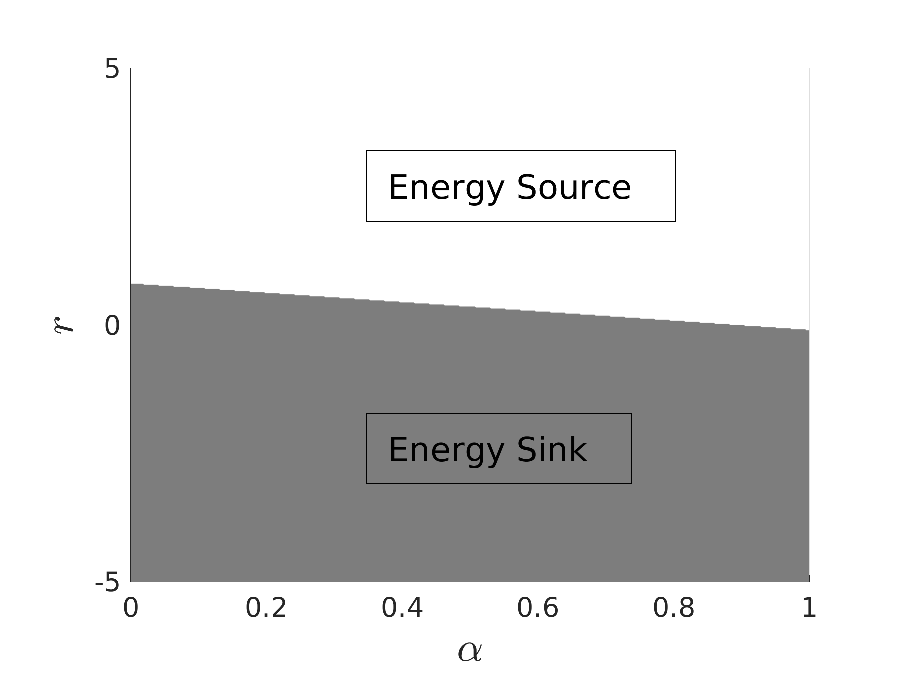
\includegraphics[width=3in]{filter_delta_energy}}
\caption{\small{Dissipative character of filtering for polynomial order $N=10$. Grey regions indicate the filter is dissipative while the white region indicates energy is being introduced into the flow by the filter.}}
\label{fig:filter_dissipation}
\end{figure}

The other aspect of the filtering operation which has been overlooked in the previous studies is its effect on the divergence-free condition. In order to asses the effects on divergence we revisit the double shear layer case studied in \cite{fischer01} and \cite{malm13}.

The flow case is setup in a two-dimensional domain $\Omega=[0,1]^{2}$ with doubly-periodic boundary conditions. The initial conditions are introduced as:
\begin{align}
 u_{0} &= 
 \begin{cases}
    	\tanh(\rho(y-0.25)),		& y \leq 0.5 \\
    	\tanh(\rho(0.75-y)),  	& y > 0.5
 \end{cases} \\
 v_{0} &= 0.05\sin(2\pi x),	\hspace{22pt}\forall\ x,y \nonumber
\end{align}
The domain is discretized with $16\times16$ spectral-element grid and each element uses $N=16$ Legendre polynomial modes, corresponding to $256$ points per element. The non-linear term is calculated using over-integration so as to preserve skew-symmetry of the advection term. The filtering stabilization procedure is also used to asses the effect of filtering on the divergence. $1\%$ of the last mode is filtered out at the end of each time-step. The tolerance of the solver for the divergence free condition is set to $10^{-10}$. Figure~\ref{fig:doubleshear_t0} shows the initial condition at time $t=0$ and Figure~\ref{fig:doubleshear_t2} shows the flow state at time $t=2$.

\begin{figure}[h]
	\centering
	\begin{subfigure}[b]{0.45\textwidth}
		\centering
		\includegraphics[width=1.1\columnwidth]{doubleshear_n16_t0}
		\caption{Initial vorticity at $t=0$}
		\label{fig:doubleshear_t0}
	\end{subfigure}
	\begin{subfigure}[b]{0.45\textwidth}
		\centering
		\includegraphics[width=1.1\columnwidth]{doubleshear_n16_t2}
		\caption{Vorticity at $t=2.0$}
		\label{fig:doubleshear_t2}
	\end{subfigure}
	\caption{Vorticity evolution for the double shear layer test case. }
	\label{fig:doubleshear_soln}
\end{figure}

Figure~\ref{fig:filter_divergence} shows the divergence of the flow field calculated before and after the application of the filter. The red line shows the divergence of the flow-filed after the pressure-correction step and the blue line indicates the divergence after the application of the filter. At the start of the simulation, when negligible energy is present in the last mode, the filter has very little impact on the divergence of the flow-field. However as the flow evolves and the energy in the smaller scales increase, violation of the divergence-free condition due to the action of the filter increases. This violation is substantial once the flow is fully developed, with the flow dropping nearly $6$ orders of magnitude in accuracy between the pressure-correction and the filtering step. This impact is surprisingly large. The case may be considered to be a stringent test with thin shear layers, which demand high resolution and thus even the small scales may contain dynamically significant energy. The situation however is representative of marginally resolved simulations where the smallest scales may still contain dynamically relevant energy, and thus filtering may have an unexpectedly large impact on the divergence-free condition of the flow-field.
\begin{figure}[h]
	\centerline{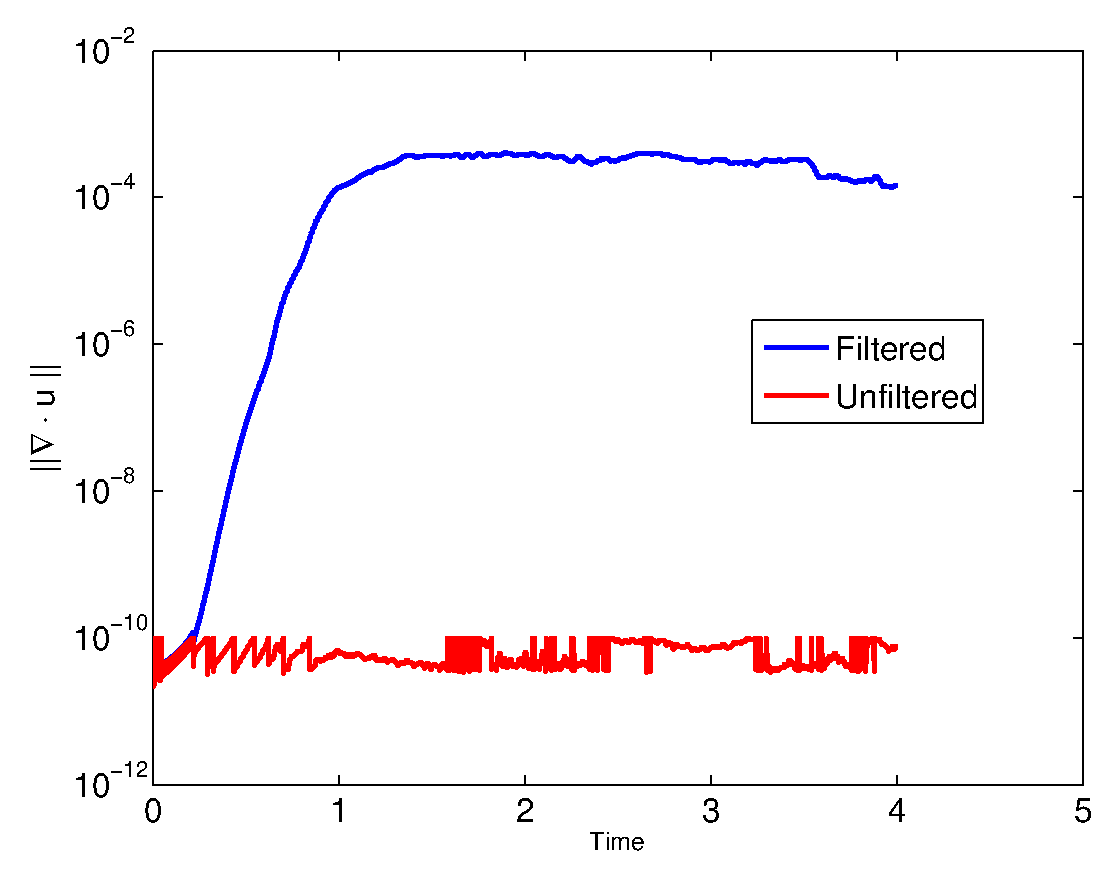
\includegraphics[width=3in]{divergence_filtered}}
	\caption{\small{The norm of the divergence after pressure correction and after filter application.}}
	\label{fig:filter_divergence}
\end{figure}

A puzzling aspect of the test as reported in the results of \cite{fischer01} and \cite{malm13} is that the case always needed some filter based stabilization. \cite{malm13} study the case with and without the use of over-integration for the non-linear term. They report that an order of magnitude lower filtering strength was needed when over-integration was used. However only over-integration did not ensure complete stabilization and the simulation experienced numerical instability at $T\sim6.7$ without filtering. \cite{malm13} attribute the destabilization to the finite accuracy of the divergence-free constraint, stating that even small errors would lead to numerical instability in the absence of dissipative terms (viscous or numerical) or stabilizing procedures (filtering). Although the authors do not report the tolerance to which the divergence free condition was satisfied. To check this again we run our test case with over-integration and without any filtering for a long duration. However contrary to the results obtained in \cite{malm13}, the simulation was stable (at least up to $T=20$). An explanation might be found when looking at the original test case reported in \cite{fischer01}. The authors there report using time steps such that the CFL number is between $1$ and $5$. The standard BDF3-K3 time-stepper would be unstable for these CFL numbers. This suggests that a characteristic time-stepping scheme may have been employed. We test the case by employing a the characteristic time-stepping scheme with over-integration but no filtering and indeed the simulation experienced numerical instabilities. This would implicate the characteristics time-stepper as the source of numerical instability. 

In retrospect, the results are to be expected. The use of consistent spaces for velocity and pressure avoids the spurious pressure oscillations. The absence of boundary conditions due to a doubly-periodic domain negates errors due to boundary terms, the use of over-integration dismisses aliasing errors as the source of instabilities and the spectral-element grid is perfectly Cartesian. Then as per the conclusion derived in \cite{malm13}, small divergence errors remain the obvious (known) source of numerical instability. However, these errors should be of the order of the specified solver tolerance for divergence. The (instantaneous) advection operator being real and skew-symmetric is a normal matrix (if evaluated completely using over-integration). Any violation of divergence-free condition of $O(\epsilon)$ can be regarded as a small perturbation to a normal matrix and one would expect a change in the eigenvalues to be of the same order $\epsilon$. Since in the ideal case the eigenvalues must lie on the imaginary axis with exactly zero real part, any perturbation due to numerical errors of order $O(\epsilon)$ would introduce new eigenvalues with a real part of $O(\epsilon)$. Thus a practical value for the solver tolerance of $10^{-8}$ would result in a advection matrix which would have eigenvalues with real parts of the order $10^{-8}$. Such a scenario creates an ever present numerical instability. However it should be an extremely weak instability, at least in such idealized test cases where other sources of instabilities are absent.

One can easily check the change of eigenvalues with varying degree of error in the advecting field. To do so we created a simple advection operator in Matlab following the spectral-element framework. A square domain with $\Omega=[0,1]^{2}$ is built and discretized using $3\times3$ spectral-elements which are further discretized using $10^{th}$ order Legendre polynomials. The advection operator is built on an over-integration grid with $19\times19$ grid points. The grid point spacing and weights for numerical integration correspond to the Gauss-Lobatto-Legendre points (GLL) for a polynomial of order $N_{d}=18$ resulting in the desired $18$ grid points for a complete integration of the convection term. Individual matrices are built independently for each spectral element and then a larger matrix for the whole system is built using direct stiffness summation. A simple sinusoidal divergence-free field can be used for building the $C\cdot\nabla$ matrix:
\begin{align}
\label{eqn:convection_op}
C_{x} &= 1.0 + 0.1\sin(2\pi x + 2\pi y) &+\epsilon\sin(2\pi x)\sin(2\pi y) \\
C_{y} &= 1.0 - 0.1\sin(2\pi x + 2\pi y) &+\epsilon\sin(2\pi x)\sin(2\pi y) \nonumber
\end{align}
When $\epsilon=0$ the field is analytically divergence free. Within the current numerical approximation the normalized divergence field defined as $||\nabla\cdot C|| = (\nabla\cdot C,\nabla\cdot C)/Volume$ is of the order $10^{-10}$. The parameter $\epsilon$ can thus be used to add a controlled perturbation to the advecting field and study the resulting change in eigenvalues. Figure~\ref{fig:spectra_eps0} and \ref{fig:spectra_eps-4} show the spectra of advection operator using $\epsilon=0$ and $\epsilon=10^{-4}$, resulting in divergence norms of the order $O(10^{-11})$ and $O(10^{-4})$ respectively. Tracking $\lambda_{max}$, defined as the eigenvalue with the largest real part, one can obtain how the instability of the advection operator changes with the variation of the divergence field. Figure~\ref{fig:lambda_dnorm} shows the change in $\lambda_{max}$ with $||\nabla\cdot C||$. As expected the trend is linear in a log-log scale with a slope of 1 across a variation of 8 orders of magnitude for $||\nabla\cdot C||$. This would suggest that relatively large divergence errors would be required for numerical instabilities to be caused by the advection term, as long as the term is evaluated completely. Of course as shown by \cite{malm13} and by \cite{kirby03}, the evaluation of this term without over-integration leads to instabilities in the absence of stabilization. These instabilities are much stronger than just divergence errors. Figure~\ref{fig:spectra_nodealias} shows the eigenvalue spectra for the advection operator (with $\epsilon=0$) evaluated on $11\times11$ GLL points in each element. The largest unstable eigenvalue is of the order $10^{-1}$, making the instability due to aliasing much stronger than the instabilities arising from the violation of the divergence-free condition.
\begin{figure}[h]
	\centering
	\begin{subfigure}[b]{0.45\textwidth}
		\centering
		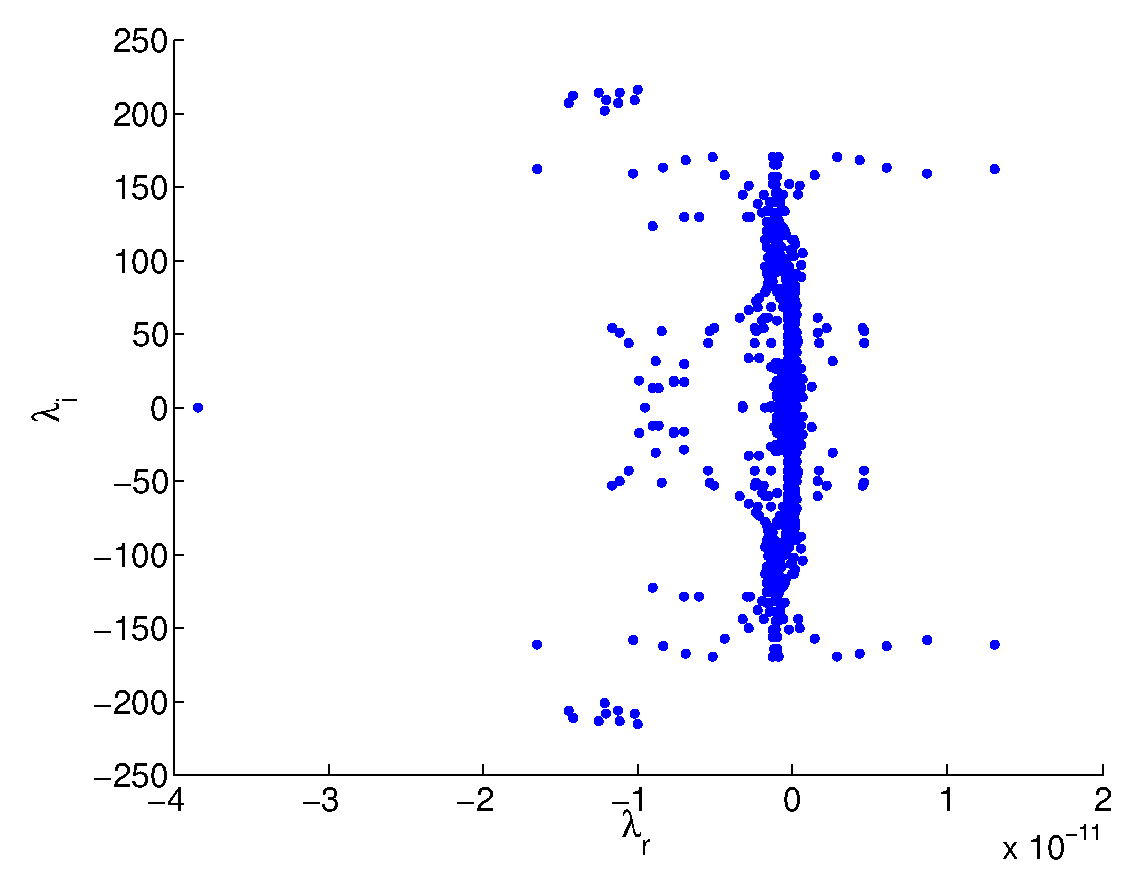
\includegraphics[width=1\columnwidth]{spectra_N10_Nxd18_nelv9_eps0}
		\caption{$||\nabla\cdot C|| \sim O(10^{-10})$}
		\label{fig:spectra_eps0}
	\end{subfigure}
	\begin{subfigure}[b]{0.45\textwidth}
		\centering
		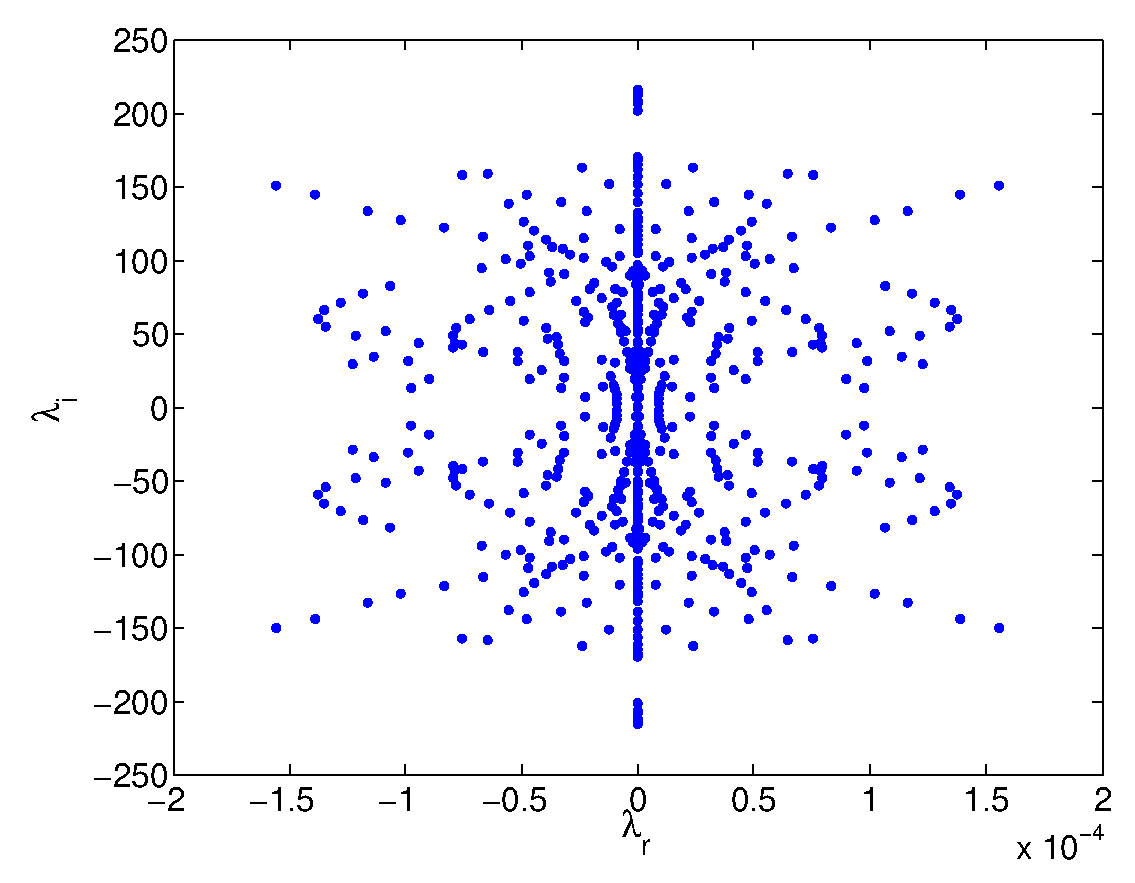
\includegraphics[width=1\columnwidth]{spectra_N10_Nxd18_nelv9_eps4}
		\caption{$||\nabla\cdot C|| \sim O(10^{-4})$}
		\label{fig:spectra_eps-4}
	\end{subfigure}
	\caption{Eigenvalue spectra for the advection operator with different divergence norms for a perturbed advecting field.}
	\label{fig:convection_spectra}
\end{figure}
\begin{figure}[h]
	\centerline{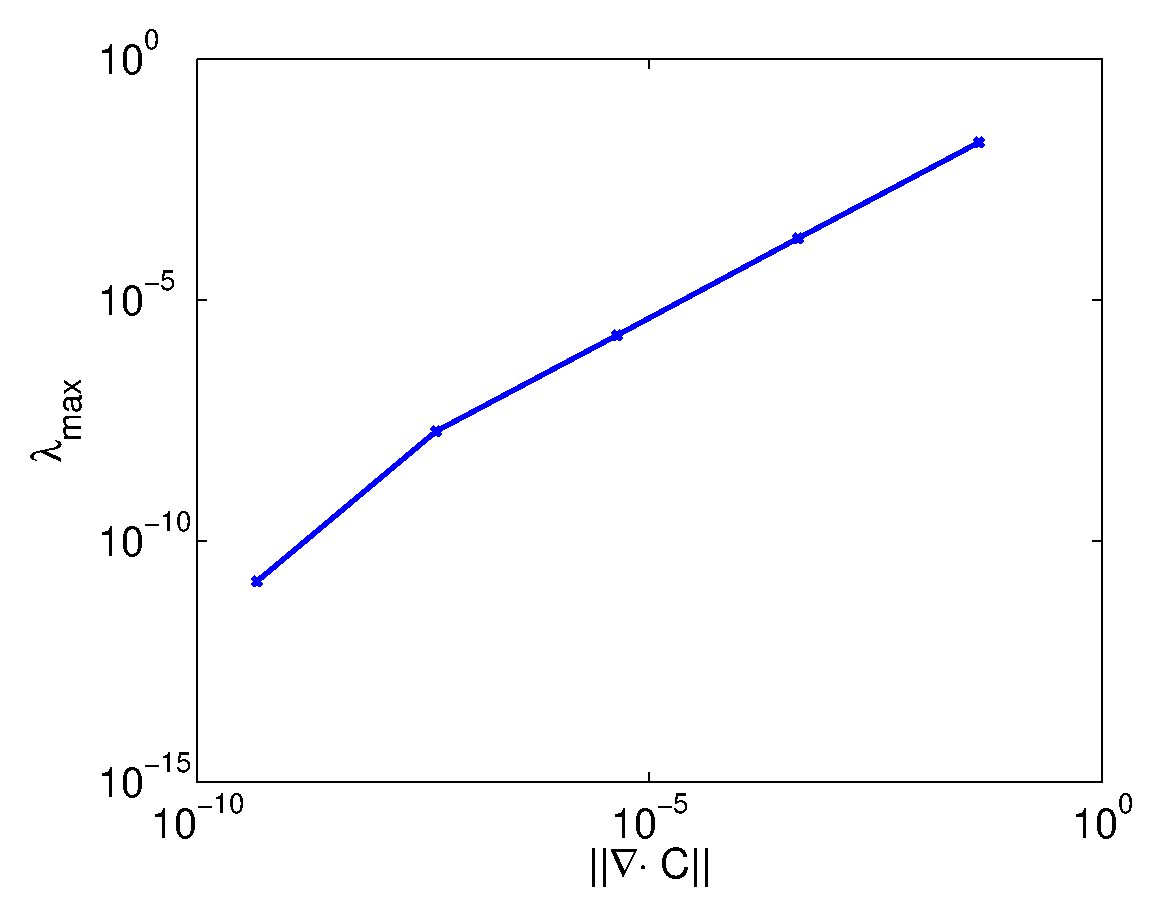
\includegraphics[width=2.5in]{N10_eig_dnorm}}
	\caption{\small{Variation of maximum real part of the eigenvalue spectrum with the norm of the divergence of the advection operator}}
	\label{fig:lambda_dnorm}
\end{figure}
\begin{figure}[h]
	\centerline{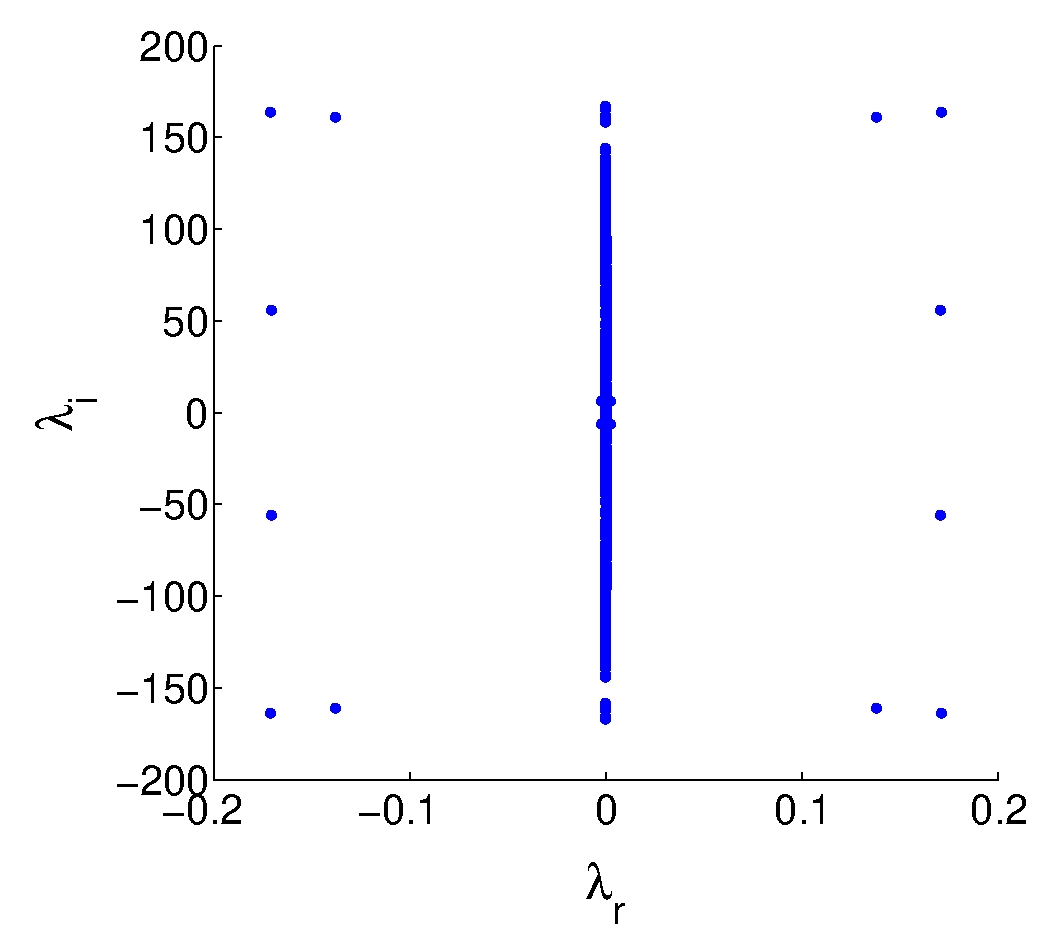
\includegraphics[width=2.5in]{spectra_nodealias_N10_Nd10}}
	\caption{\small{Eigenvalues for the advection term evaluated without over-integration}}
	\label{fig:spectra_nodealias}
\end{figure}
\cite{malm13} found that for the double shear layer case, the numerical instabilities first manifested in the thinnest part of the shear layers, thus concluding high shear regions necessarily need numerical stabilization. Since we do not experience any numerical instabilities using the BDF-EXT-k time stepping scheme, we further test this conclusion by reducing the resolution for the test case. We run the simulation with the same $16\times16$ spectral-elements but with polynomial orders of $N=11,7$ and $5$. These would lead to under-resolved shear layers. The under-resolution is strongly visible in the flow-field for the lowest polynomial order case of $N=5$. Figure~\ref{fig:vorticity_n6_t1} shows the vorticity in the flow field at time $t=1.0$ for $N=5$. However in all cases we find that the simulation does not experience any numerical instabilities (at least up till $t=20$) and additional stabilization was not required. The results indicate that in the absence of boundary terms and other sources of errors, under-resolution alone may not lead to numerical instabilities as long as the flow-field divergence remains small and the non-linear term is evaluated using complete over-integration. These results are consistent with those presented by \cite{kirby03} who found that they were able to simulate transition and turbulence in triangular ducts as well as turbulent channel flow simulations after employing over-integration but without additional flow stabilization.
\begin{figure}[h]
	\centering
	\includegraphics[width=3.5in]{doubleshear_n6_t1}
	\caption{\small{Vorticity at $t=1.0$ for the double shear layer case using polynomial order $N=5$}}
	\label{fig:vorticity_n6_t1}
\end{figure}


\section{Relaxation-term based stabilization}

In practical simulations over-integration errors may not be the only source of numerical instability and often it is found that simulations, especially those involving complex geometries or truncated domains require some amount to stabilization despite the use of over-integration. Filter-based stabilization has been an effective and efficient method to suppress such numerical instabilities. However the results of the previous section highlight some of the drawbacks of such a procedure. The loss of divergence free condition may be particularly severe for marginally resolved cases. In such a scenario, one may wish to look for an alternative method which preserves the advantages of explicit filtering, namely, efficiency and simplicity, while doing away with the potential drawbacks. One possible alternative in the context of the pressure-correction method is to perform the filtering procedure before the pressure-correction step. In the standard algorithm, the pressure-correction would follow a three-step procedure as follows: 
\begin{itemize}
	\item Velocity prediction $\rightarrow$ Pressure correction $\rightarrow$ Filtering.
\end{itemize}
A modified procedure would then follow:
\begin{itemize}
	\item Velocity prediction $\rightarrow$ Filtering $\rightarrow$ Pressure Correction.
\end{itemize}
This allows the filtering of the highest scales but leaves the solution unchanged after the divergence-free condition has been enforced. Such a procedure would remedy perhaps the most striking drawback of explicit filtering, which is the loss of divergence, while still retaining the simplicity and efficiency of explicit filtering operation. However the other drawbacks mentioned earlier, \textit{i.e} time-step dependence of filtered energy and the statistical nature of filter dissipation, still remain.

As it would turn out, there is an equally simple method that can resolve all the above mentioned deficiencies and is analogous to performing an explicit filtering procedure. As has been pointed out in \cite{stolz01} and \cite{schlatter04}, doing an explicit filtering operation is equivalent to doing an implicit time-relaxation. Formally, the two may be shown to be equivalent using a simple evolution equation \ref{eqn:NL_evolution}.
\begin{align}
\frac{\partial u}{\partial t} + \mathcal{F}(u) = 0
\label{eqn:NL_evolution}
\end{align}
Where $\mathcal{F}(u)$ is a (possibly non-linear) evolution operator.
The explicit filtering procedure may then be shown using a simple semi-discretized form of the evolution equation:
\begin{align}
u^{*} = u^{n} - \mathcal{F}(u^{n})\Delta t + O(\Delta t^{2})\nonumber \\
u^{n+1} =  \mathcal{G}(u^{*}) %& (\mathcal{G} - \text{Low pass filter.})
\label{eqn:NL_evolution_filtered}
\end{align}
Where $\mathcal{G}$ is a defined low-pass filter. As an alternate method, one may consider the same evolution equation supplemented by a relaxation-term as in equation~\ref{eqn:NL_evolution_rt}:
\begin{align}
\frac{\partial u}{\partial t} + \mathcal{F}(u) = \boldsymbol{-\chi \mathcal{H}(u)}
\label{eqn:NL_evolution_rt}
\end{align}
Which may be evolved using a time-splitting scheme:
\begin{align}
u^{*} = u^{n} -\mathcal{F}(u)\Delta t + O(\Delta t^{2})	\nonumber \\
u^{n+1} = u^{*} -\chi \mathcal{H}(u^{*})\Delta t + O(\Delta t^{2})
\label{eqn:NL_evolution_rt_1}
\end{align}
Taking the the parameter $\chi=1/\Delta t$ and $\mathcal{H}=\mathcal{(I-G)}$ to be the corresponding high-pass filter of $\mathcal{G}$, and substituting in equation \ref{eqn:NL_evolution_rt_1} one obtains:
\begin{align}
u^{n+1} = \mathcal{G}(u^{*}) + O(\Delta t^{2})
\label{eqn:NL_evolution_rt_2}
\end{align}
which is equivalent to the expression obtained in equation \ref{eqn:NL_evolution_filtered} to leading order of time discretization. \cite{stolz01} and \cite{schlatter04} interpret the relaxation-term as performing an equivalent low-pass filtering operation $\mathcal{G}$ every $1/(\chi\Delta t)$ time-steps. Alternately one may interpret this to mean that the relaxation-term procedure is equivalent to performing an explicit filtering operation with a filter strength of $(\chi\Delta t)$. 

Thus the ``filter-based stabilization'' operation proposed by \cite{fischer01} may be reformulated as an equivalent ``relaxation-term-based stabilization'', which we refer to as ``RT stabilization''. It can be easily incorporated into the Navier-Stokes by a simple addition of a relaxation-term on the right hand side. Thus the equivalent RT stabilized equation may be written as:
\begin{align}
\frac{\partial u}{\partial t} + u\cdot\nabla u = -\frac{\nabla p}{\rho} + \nu\nabla^{2}u -\chi\mathcal{H}(u) \\
\nabla\cdot u = 0
\label{eqn:rt_NS}
\end{align}
Where $\mathcal{H}(u)$ is a high-pass-filtered velocity field. The parameter $\chi$ may be used as a weighting parameter similar to the filter weight `$\alpha$' used in \cite{fischer01} and \cite{malm13}. Such a formulation immediately provides us with two advantages over the explicit filtering operation. Firstly, since there are no more explicit filtering operations after the pressure-correction step, the velocity field remains divergence free. Secondly, with the RT now part of the evolution equations, for a fixed $\chi$ and $\mathcal{H}$ the physical energy drain provided by the RT should be independent of the chosen time-step (as long as numerical stability is ensured). The final aspect of the stabilization concerning the dissipative character of the RT requires more constraints. When $\mathcal{H}$ is chosen to be positive semi-definite, and $\chi$ is a positive constant, the relaxation-term is purely dissipative. However with spatially varying $\chi$ and $\mathcal{H}$ the relaxation-term may be non-dissipative \citep{stolz03}.
\subsection{RT parameters}
\cite{malm13}, in the context of spectral-elements, describe a simple transfer function $\mathcal{G}$ defined for a variable in a one-dimensional domain $\Omega=[-1, 1]$ such that the filtering operation takes the simple form: 
\begin{align}
\bar{u}_{N}(x) = \mathcal{G}(u_{N}(x)) = \sum_{k=0}^{N}\sigma_{k}a_{k}\phi_{k}(x)
\end{align}
Where $\phi_{k}$ is the basis function and the definition of $\sigma_{k}$ describes the low-pass filter function $\mathcal{G}$ which takes the form:
\begin{align}
\sigma_{k} &=
	\begin{cases}
	1 - \alpha\left(\frac{k-k_{c}}{N-k_{c}}  \right)^{2}, & k>k_{c} \\
	1, & k\le k_{c}
	\end{cases}
\end{align}
Where $N$ is the number of modes in the spectral-element discretization and $k_{c}$ is the cut-off mode in spectral space used for building the filter. Amplitudes for modes $k\le k_{c}$ are unaffected by the filter operation. $\alpha$ is the filter weight such that $0\le\alpha\le1$. In keeping with our analysis earlier, we may define the corresponding high-pass filter $\mathcal{H}$ for the RT as:
\begin{align}
\mathcal{H}(u_{N}(x)) &= \sum_{k=0}^{N}\gamma_{k}a_{k}\phi_{k}(x) \\
\gamma_{k} &=
\begin{cases}
	\left(\frac{k-k_{c}}{N-k_{c}}  \right)^{2}, & k>k_{c} \\
	0, & k\le k_{c}
\end{cases}
\end{align}
Where the parameter $\alpha$ is absorbed into $\chi$ which acts as an RT strength term. To formally have the same operation as the explicit filter, the value of $\chi$ can be set to $\chi=(\alpha/\Delta t)$. This is in agreement with our earlier interpretation that the RT procedure is equivalent to performing a low-pass filter operation every time-step with a strength of $(\chi\Delta t)$. Using this value we get $\chi\Delta t = \alpha$ and thus we recover the correct weighting for the equivalent explicit filter operation. 

The basis functions $\phi$ used for the definition of $\mathcal{H}$ however is different from the one used by \cite{malm13} who use the transformed basis functions described by \cite{boyd98} which are described in equation~\ref{eqn:boyd}. Using this basis function however, the form of $\mathcal{H}$ is not semi-positive definite and thus the relaxation term is not purely dissipative. This is rather expected from our earlier results which show that the explicit filter operation using such a transformed basis has a substantial parameter range where it acts as an energy source. The equivalent RT formulation then can not be purely dissipative. We use the Legendre polynomials as the basis functions (for a Legendre-spectral-element method) for building the RT which makes $\mathcal{H}$ semi-positive definite. Thus for $\chi>0$ the relaxation term $-\chi\mathcal{H}(u)$ is always purely dissipative.

\subsection{Stability and parameter range}
The action of the RT can be inferred from the change in eigenvalues of the system due to the added stabilization. As an illustration we build the system matrices using the simple $3\times3$ spectral-element grid in Matlab for a linear advection operator stabilized by a relaxation-term. The advection operator is built using the parameters in equation~\ref{eqn:convection_op}. We set $\epsilon=10^{-2}$ so that the operator now models a numerically unstable system with positive eigenvalues. The eigenvalues of the unstable system without the addition of a relaxation term are shown in figure~\ref{fig:spectra_conv_eps2}. As expected, there are unstable eigenvalues with positive real part of order $O(10^{-2})$. With the addition of an RT as defined earlier, with $k_{c}=10$ and $\chi=0.4$ causes the eigenvalues to shift towards the negative real plane (figure~\ref{fig:spectra_rhs_eps2}). In the example shown here, the instability appears to be completely suppressed and the largest real part of the eigenvalues of the resulting system is zero. The overall system is more dissipative as evidenced by the general negative shift of the real part of the eigenvalues.
\begin{figure}[h]
	\centering
	\begin{subfigure}[b]{0.45\textwidth}
		\centering
		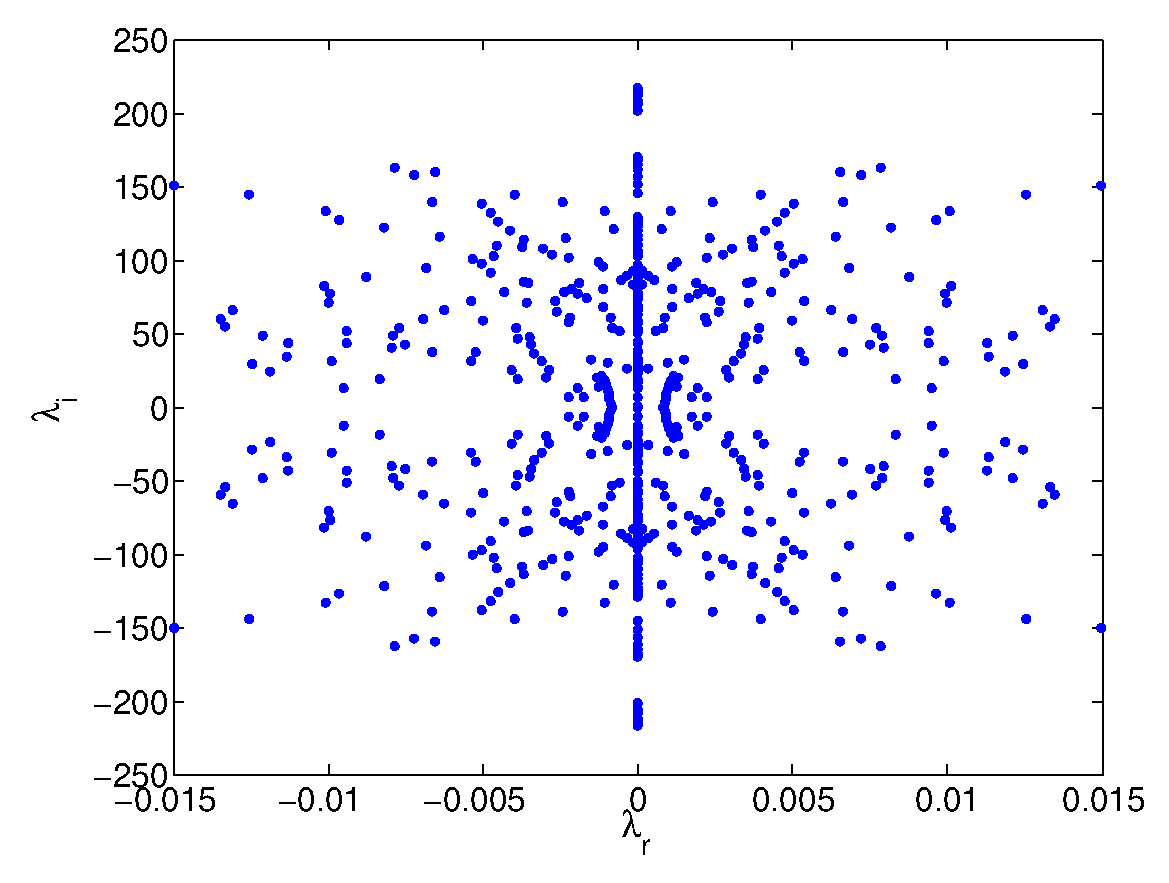
\includegraphics[width=1\columnwidth]{spectra_conv_N10_Nxd18_nelv9_eps2}
		\caption{$||\nabla\cdot C|| \sim O(10^{-2})$}
		\label{fig:spectra_conv_eps2}
	\end{subfigure}
	\begin{subfigure}[b]{0.45\textwidth}
		\centering
		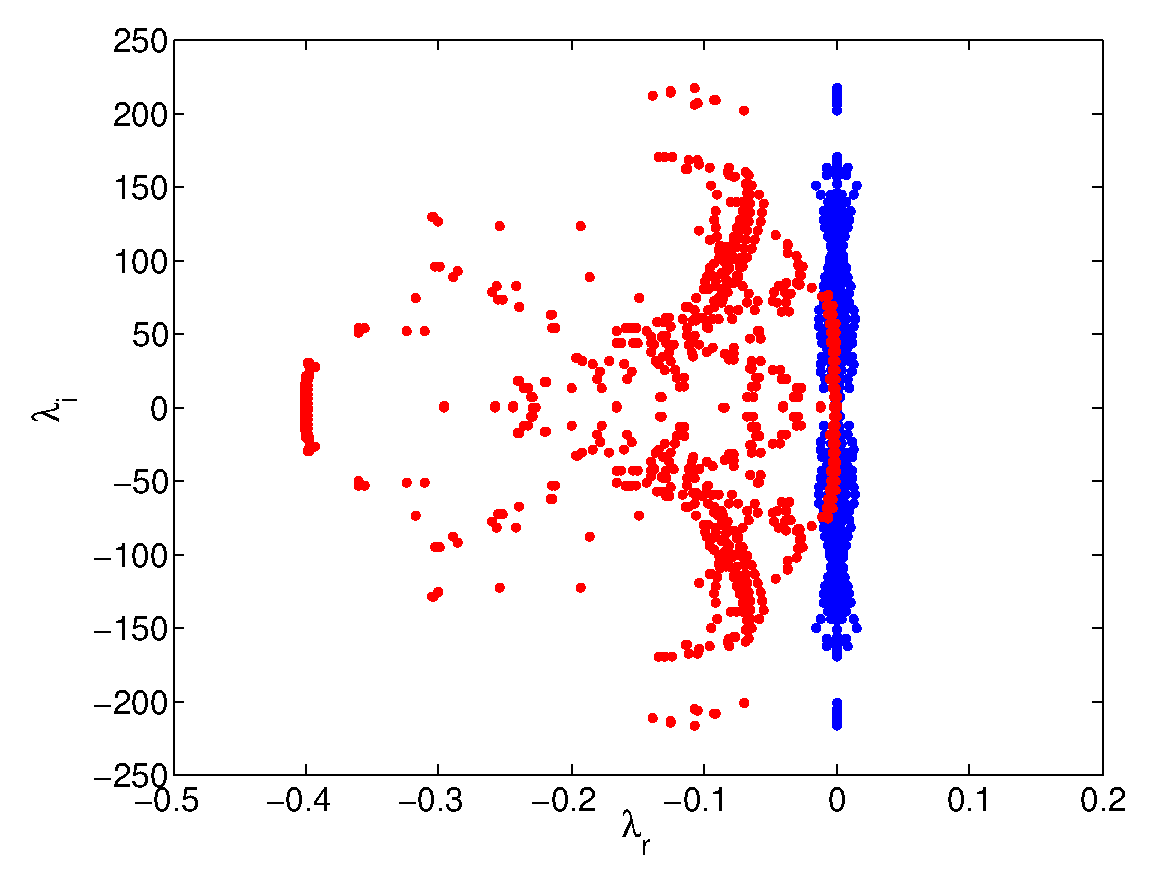
\includegraphics[width=1\columnwidth]{spectra_rhs_N10_Nxd18_nelv9_eps2}
		\caption{Stabilized Eigenvalues.}
		\label{fig:spectra_rhs_eps2}
	\end{subfigure}
	\caption{Comparison of eigenvalues for an unstable system (a) with $||\nabla\cdot C|| \sim O(10^{-2})$ and a system stabilized using a relaxation-term (b)}
	\label{fig:rt_spectra}
\end{figure}

While the RT clearly has a stabilizing effect on the system, it can also be destabilizing for a certain range of parameters. From figure~\ref{fig:spectra_rhs_eps2} one can notice some eigenvalues of the stabilized system have a large negative shift with the smallest real part being $\lambda_{r}^{min}=-0.4$. As it turns out this particular eigenvalue sets the stability limits of the RT stabilization approach. For a particular temporal discretization such as the BDF-EXT-3, the region of stability may cover a finite region of the negative plane. For a system with eigenvalues such that $\lambda\Delta t$ falls outside the stability region of the time-stepping scheme, the system becomes numerically unstable. The scaled eigenvalues with varying values of the parameter $\chi\Delta t$ (and $k_{c}=1$) are shown in figure~\ref{fig:rt_stability} with a black line enveloping the region of stability for a BDF-EXT-3 temporal discretization scheme. As the strength of the RT stabilization is increased by varying $\chi$, the eigenvalues become more negative and the dissipative character of the stabilization procedure becomes stronger. Eventually as $\chi\Delta \approx 1$ the stabilization procedure itself becomes numerically unstable and the time-step needs to be reduced in order to render the simulation numerically stable again. The analysis is exemplified using the BDF-EXT-3 scheme but the concept generalizes to other schemes and the limit of stability will be governed by the stability region of the respective schemes.
\begin{figure}[h]
	\centering
	\begin{subfigure}[b]{0.45\textwidth}
		\centering
		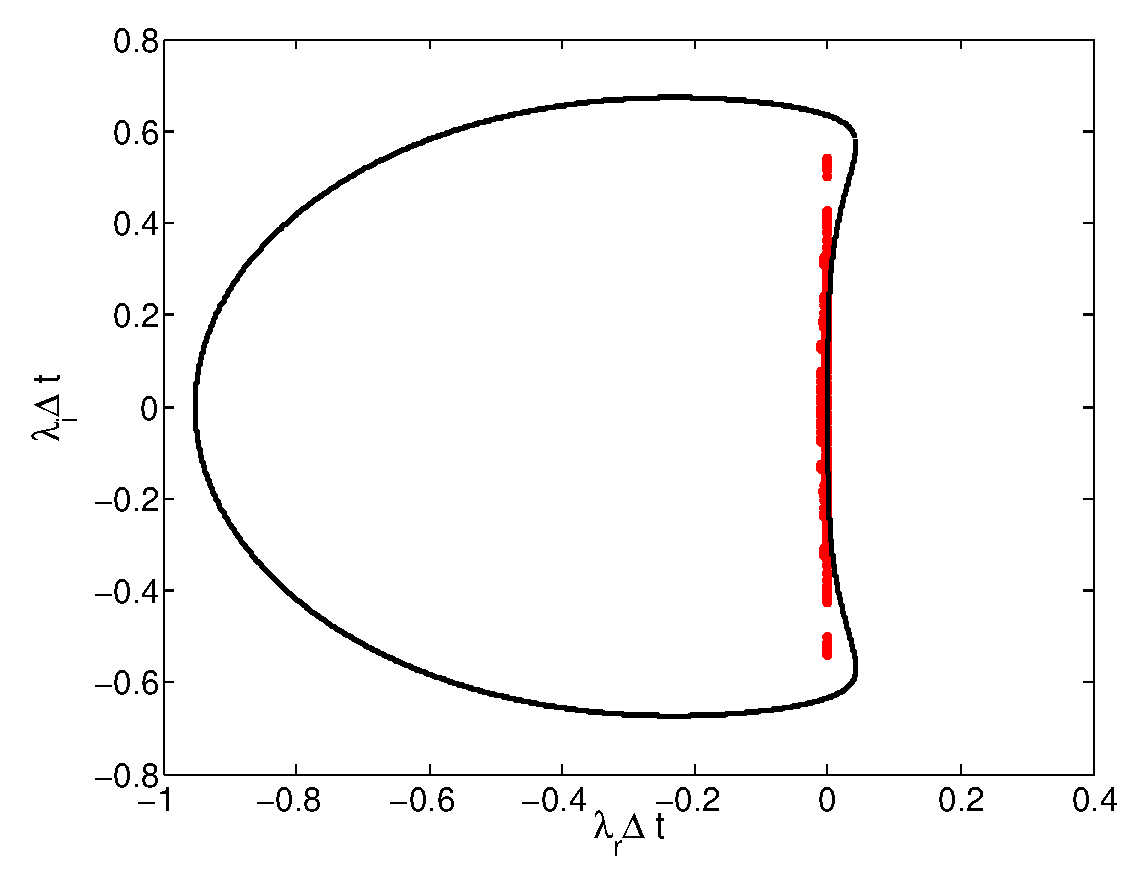
\includegraphics[width=1\columnwidth]{spectra_chidt_001}
		\caption{$\chi\Delta t=0.01$}
		\label{fig:spectra_chidt001}
	\end{subfigure}
	\begin{subfigure}[b]{0.45\textwidth}
		\centering
		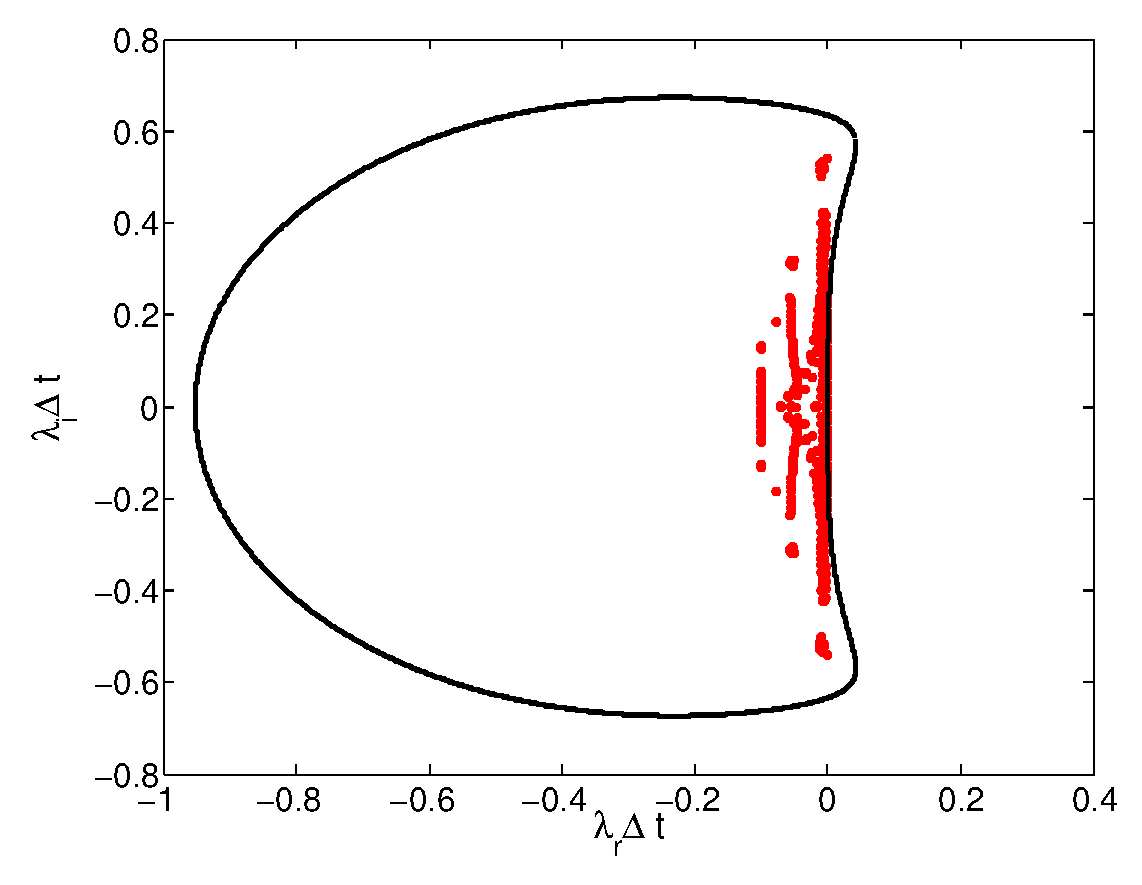
\includegraphics[width=1\columnwidth]{spectra_chidt_010}
		\caption{$\chi\Delta t=0.10$}
		\label{fig:spectra_chidt01}
	\end{subfigure}
	\begin{subfigure}[b]{0.45\textwidth}
		\centering
		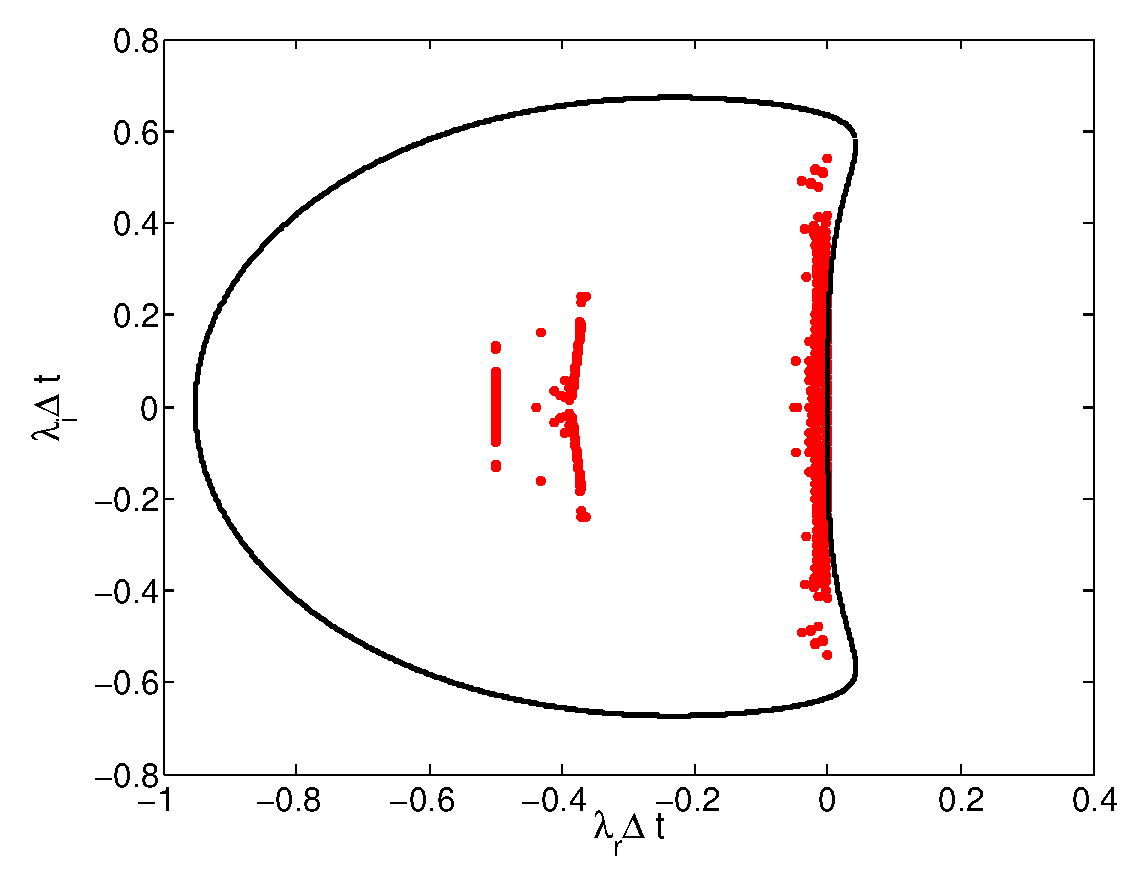
\includegraphics[width=1\columnwidth]{spectra_chidt_050}
		\caption{$\chi\Delta t=0.50$}
		\label{fig:spectra_chidt050}
	\end{subfigure}
	\begin{subfigure}[b]{0.45\textwidth}
		\centering
		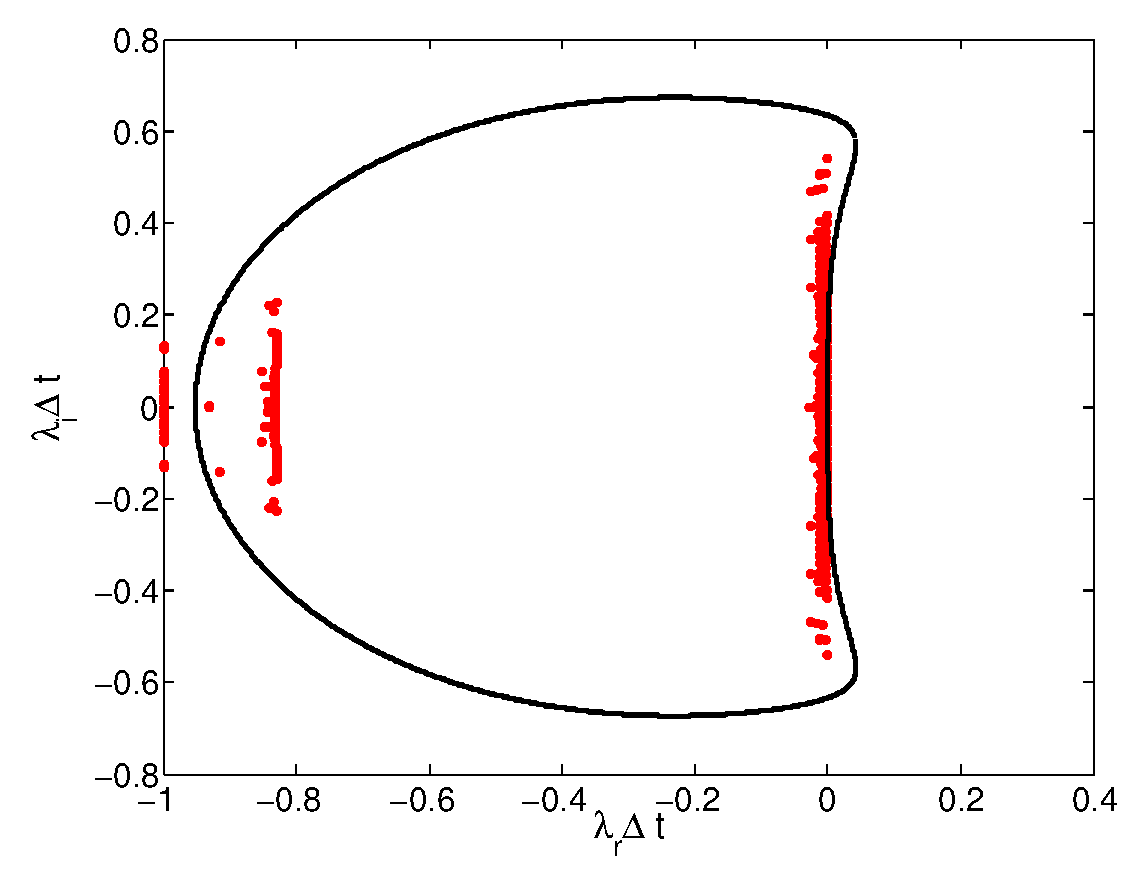
\includegraphics[width=1\columnwidth]{spectra_chidt_100}
		\caption{$\chi\Delta t=1.00$}
		\label{fig:spectra_chidt100}
	\end{subfigure}	
	\caption{Changes in eigenvalues with varying filter strength $\chi\Delta t$ with $k_{c}=10$.}
	\label{fig:rt_stability}
\end{figure}
This condition limits the parameter range for which a relaxation-term type stabilization can be used. Practical values of the $\chi$ parameter should not reach such a limit. To compare with an explicit filtering case, practical values of the filter strength vary between $0\le\alpha\le0.3$ which correspond to $0\le\chi\Delta t\le0.3$. \cite{fischer01} apply the filtering procedure with $\alpha=1.0$ and note that lower values of $\alpha$ are preferable. Should one find that the dissipation provided at low values of $\chi$ is not enough, the alternative would be to change the cut-off wavenumber $k_{c}$. This increases the added dissipation by the relaxation-term but does not substantially change the stability limits. Figure~\ref{fig:rt_stability_k8} shows the change in eigenvalues with different $\chi\Delta t$ using the cut-off mode number as $k_{c}=8$. The system is clearly more dissipative with many more eigenvalues with large negative real parts. However the approach to numerical instability remains approximately the same at $\chi\Delta t\approx 1.0$.
\begin{figure}[h]
	\centering
	\begin{subfigure}[b]{0.45\textwidth}
		\centering
		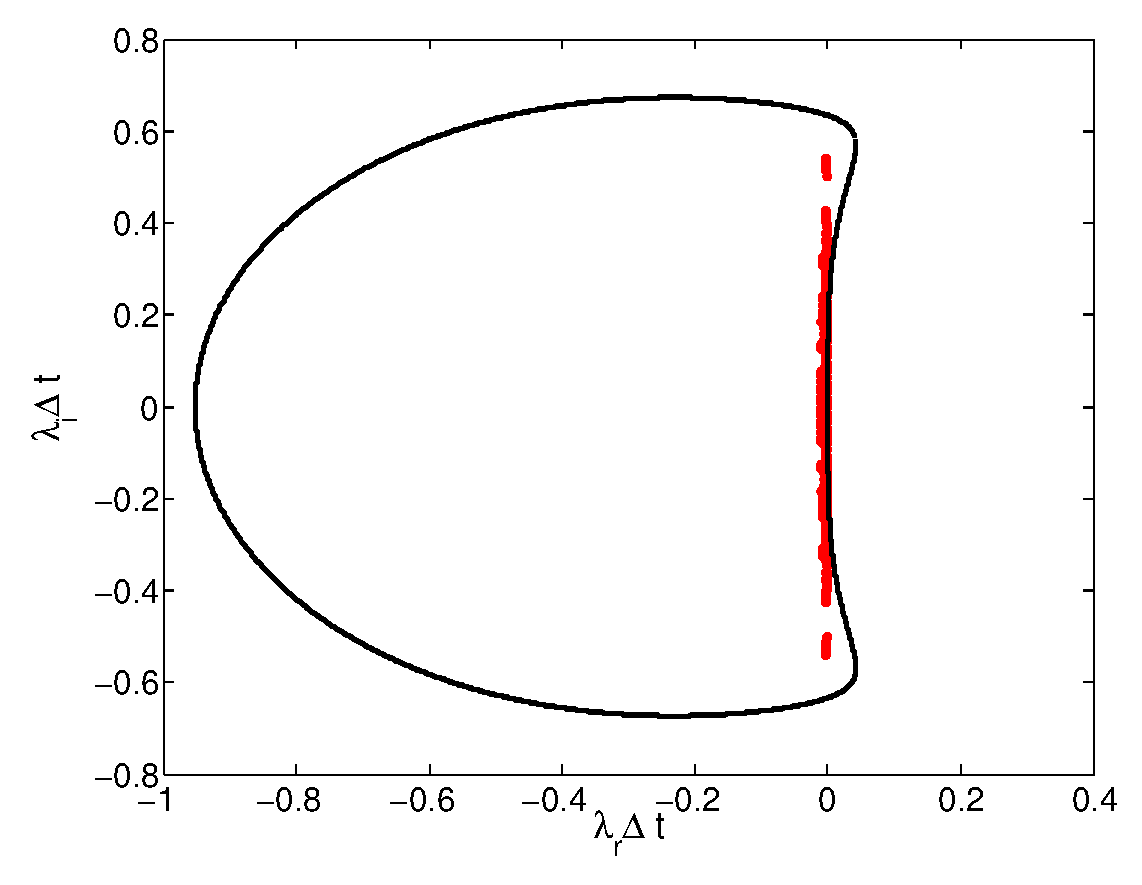
\includegraphics[width=1\columnwidth]{spectra_chidt_001_k8}
		\caption{$\chi\Delta t=0.01$}
		\label{fig:spectra_chidt001_k8}
	\end{subfigure}
	\begin{subfigure}[b]{0.45\textwidth}
		\centering
		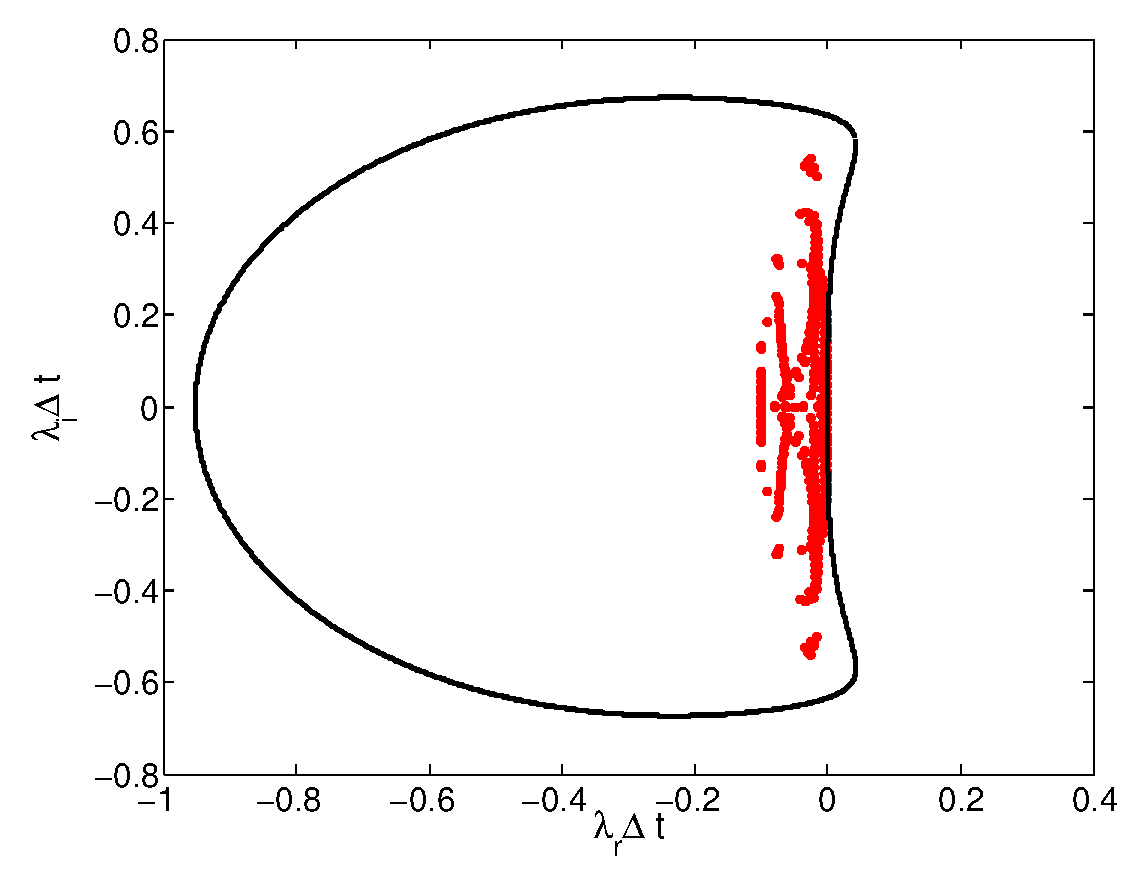
\includegraphics[width=1\columnwidth]{spectra_chidt_010_k8}
		\caption{$\chi\Delta t=0.10$}
		\label{fig:spectra_chidt01_k8}
	\end{subfigure}
	\begin{subfigure}[b]{0.45\textwidth}
		\centering
		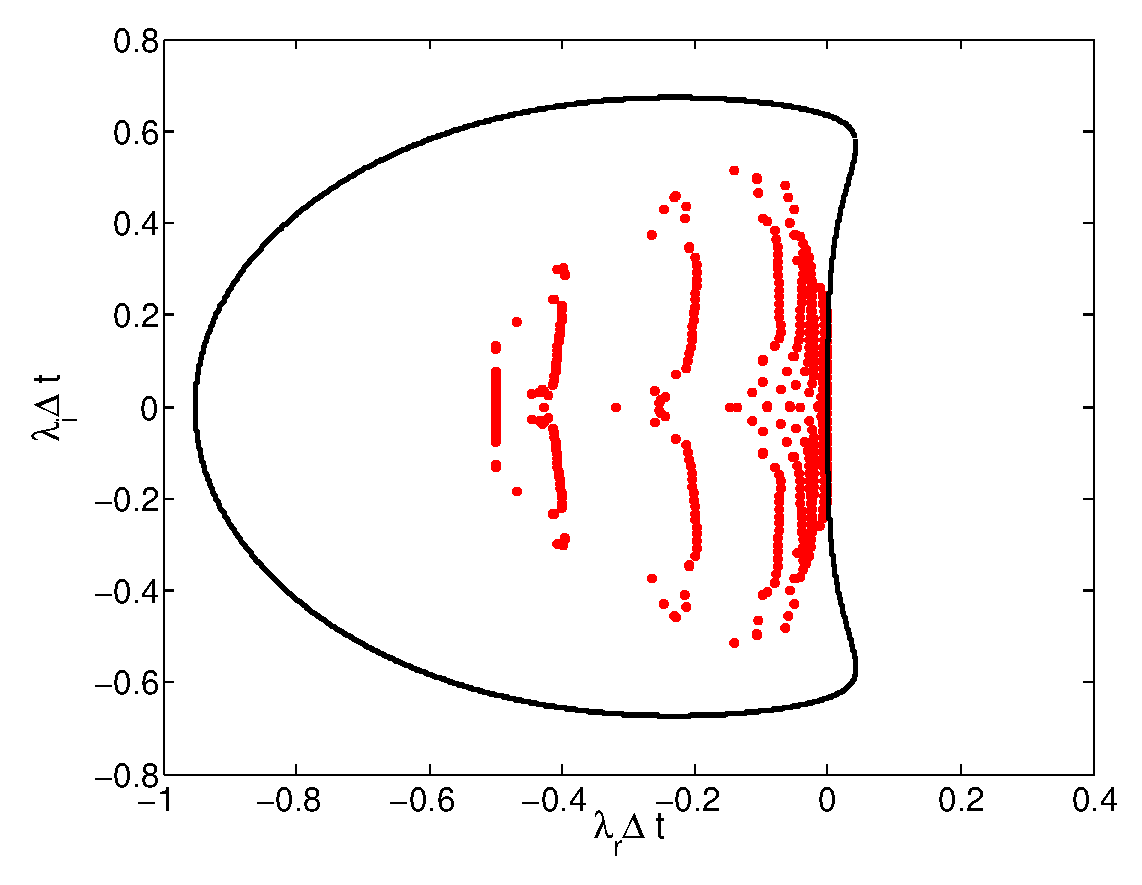
\includegraphics[width=1\columnwidth]{spectra_chidt_050_k8}
		\caption{$\chi\Delta t=0.50$}
		\label{fig:spectra_chidt050_k8}
	\end{subfigure}
	\begin{subfigure}[b]{0.45\textwidth}
		\centering
		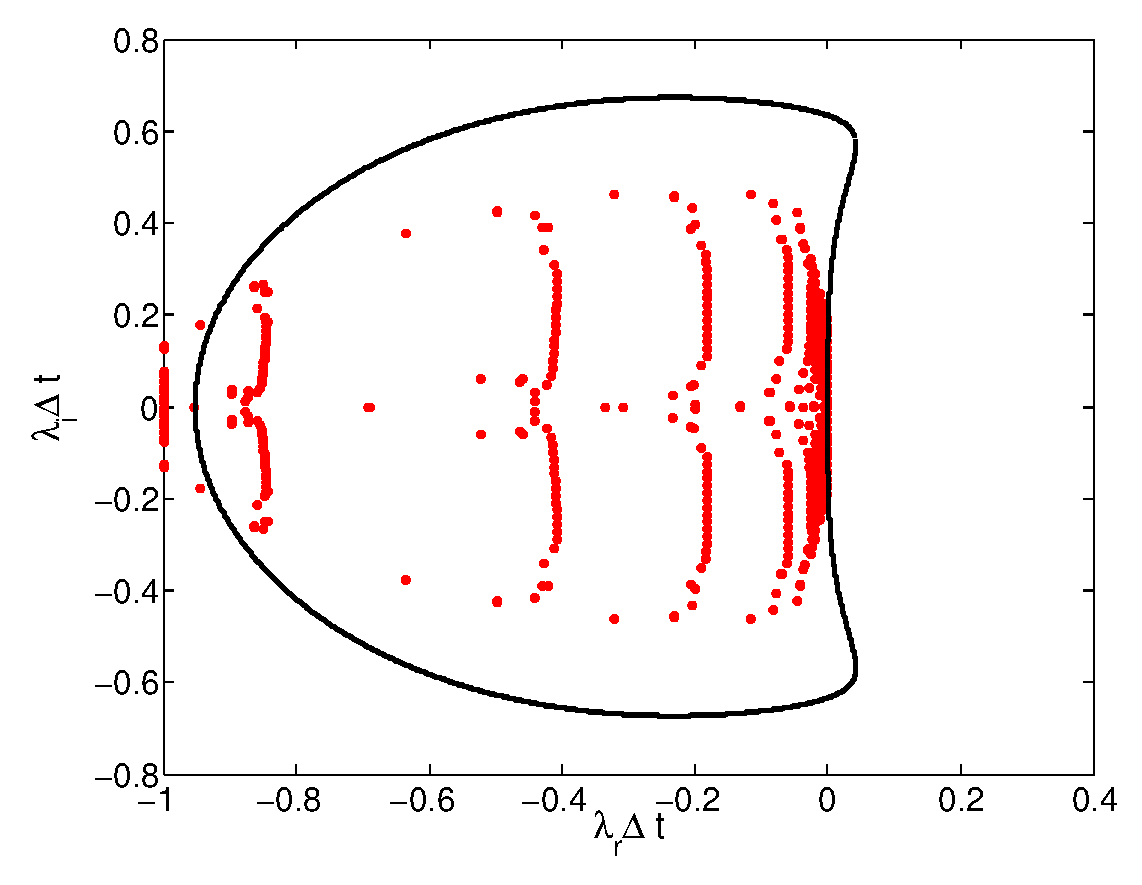
\includegraphics[width=1\columnwidth]{spectra_chidt_100_k8}
		\caption{$\chi\Delta t=1.00$}
		\label{fig:spectra_chidt100_k8}
	\end{subfigure}	
	\caption{Changes in eigenvalues with varying filter strength $\chi\Delta t$ with $k_{c}=8$.}
	\label{fig:rt_stability_k8}
\end{figure}

It is important to note that such a formulation is very similar to the RT-3D approach used by \cite{schlatter04} in the context of large-eddy simulations of transitional flows. In the study the authors compare different variants of the ADM-RT (approximate deconvolution model with relaxation term) for transitional and turbulent regimes. In the RT-3D variant the non-linear terms are computed without the deconvolution procedure and hence only the relaxation-term is used for modeling the sub-grid stresses. In the current study we are only concerned with the relaxation-term procedure in the context of numerical stabilization. 

\subsection{Double shear layer}
We test the RT stabilization in the 2D model test case of double shear layer as done in by \cite{fischer01} and \cite{malm13} for a several different parameters. Quite expectedly the procedure successfully stabilizes the simulations. We show the results of only one test case when no over-integration is employed, which would be the most stringent test case for stabilization. We ran the test using a $16\times16$ spectral-element grid with $N=16$ Legendre modes in each spectral-element. The RT parameters of $\chi=1.5\times10^{-3}$ (corresponding to $\chi\Delta t=0.3$) and $k_{c}=15$ were used. Figure~\ref{fig:rt_n15_t2} shows the vorticity in the field at $t=2.0$ where the thin shear layers are clearly visible. The simulation ran without numerical instabilities up to $t=20$.
\begin{figure}[h]
	\centering
	\includegraphics[width=3.0in]{visit_rt_t2}
	\caption{\small{Vorticity at $t=2.0$ for the double shear layer case using polynomial order $N=16$ without over-integration and using a relaxation-term stabilization.}}
	\label{fig:rt_n15_t2}
\end{figure}


\section{Conclusion}
We reassess the filter-based stabilization proposed by \cite{fischer01} and find that despite its appealing simplicity and efficiency, it suffers from several drawbacks, the most striking of which is the loss of the divergence-free condition of the flow field. In marginally resolved simulations, this loss may be severe as in our model test case where 6 orders of accuracy was lost for the divergence-free condition. Two other drawbacks are the time-step dependence of the filtered energy and the statistical character of the filter dissipation. An alternate formulation for stabilization is proposed called the ``relaxation-term-based stabilization'' or RT stabilization, which is closely related to the explicit filtering operation. With appropriate parameters can be shown to be equivalent to an explicit filter operation to leading order of time discretization. The procedure stabilizes the numerical method without destroying the divergence-free condition and for an appropriately built high-pass filter $\mathcal{H}$ the term has the quality of being purely dissipative. Moreover, the stabilization is now part of the evolution equations, and thus the energy drain due to relaxation-term is independent of the chosen time-step. Limits of the stabilization are also shown and under certain parameters the stabilization itself becomes numerically unstable. However the procedure is stable under the standard parameter ranges which may be expected for numerical stabilization. Test cases with the double shear layer shows the relaxation-term is able to stabilize the numerical simulation even in the absence of over-integration, which corresponds to a fairly stringent case of numerical stability in the presence of negligible viscosity.




%\begin{footnotesize}
%\bibliography{licentiate}\bibliographystyle{jfm}
%\end{footnotesize}

%\end{document}



%------------------------------------------------------------------------------
% Bibliography
%------------------------------------------------------------------------------
%
%\clearpage
\bibliographystyle{jfm}
\bibliography{licentiate}
%
%\IfFileExists{stabilization/paper.bbl}{%------------------------------------------------------------------------------
% Define title, author(s), affiliation and publishing status
%
\papertitle[Rexalation-term stabilization] % Short title used in headlines (optional)
{%
  A re-examination of filter-based stabilization for spectral element methods% THE COMMENT SYMBOL AT THE END OF THIS LINE IS NEEDED
}%
%
\papertoctitle{Relaxation-term-based stabilization} % Title for toc
%
\paperauthor[Negi P. S.] % Short authors used in headlines and List Of Papers
{%
  P. S. Negi %$^{1,2}$, P. Schlatter$^{1,2}$, A. Hanifi$^{1}$ and D. S. Henningson$^{1,2}$%
}%
%
%\listpaperauthor{A. Skywalker \& D. Vader}% (optional) Short authors used in List Of Papers
%
\paperaffiliation
{%
%  $^1$ Linn\'e FLOW Centre, KTH Mechanics, S-100 44 Stockholm, Sweden\\
%  $^2$ Swedish e-Science Research Centre (SeRC), SE-100 44, Stockholm, Sweden%
  Linn\'e FLOW Centre, KTH Mechanics, S-100 44 Stockholm, Sweden\\
  Swedish e-Science Research Centre (SeRC), SE-100 44, Stockholm, Sweden%
}%
%
\paperjournal[Gal. Empire Publ.] % Short publish info used in List Of Papers
{%
	Galactic Empire Publications%
}%
%
\papervolume{42}%
%
\papernumber{2}%
%
\paperpages{1--10}%
%
\paperyear{3639}%
%
\papersummary%
{% Insert summary of the paper here (used in introduction) 
	The implications of concurrent archetypes have been far-reaching and
	pervasive. Given the current status of heterogeneous technology,
	cyberinformaticians daringly desire the key unification of the Turing
	machine and erasure coding. We explore new decentralized information,
	which we call Tuna.
}%
%
\graphicspath{{stabilization/imgs/}}%
%
%
%===============================================================================
%                            BEGIN PAPER
%===============================================================================
%
\begin{paper}

\makepapertitle

%------------------------------------------------------------------------------
% Abstract
%------------------------------------------------------------------------------
%
\begin{paperabstract}
	We revisit the ``filter-based stabilization'' approach proposed by \cite{fischer01} and find that it suffers from several drawbacks. In particular the ``evolve and filter'' approach causes a violation of the divergence-free condition which can be particularly severe in the cases of marginally resolved flows. Moreover the form of the filtering operation causes the filter to not be purely dissipative. Instead of a filter-based approach we propose to use a ``relaxation-term-based stabilization'' which we refer to as an RT stabilization, which is very closely related to the explicit filtering operation. The method retains the advantages of simplicity and efficiency of a filter based approach while also remedying the above mentioned drawbacks. Parameter limits of such a stabilization procedure are explored and the method is shown to be effective within the practical parameter ranges.
\end{paperabstract}


%------------------------------------------------------------------------------
% Article
%------------------------------------------------------------------------------
%

\section{Introduction}

 Stability of numerical methods is a well-known challenge. This is particularly true in the case of high Reynolds number (R$e$) flows where low physical dissipation, combined with the low dissipation provided by the numerical method, allows small numerical errors to grow in time. A particular type of instability arises  due to the violation of the \emph{inf-sup} or Ladyzenskaya-Brezzi-Babu\v{s}ka (LBB) condition. These instabilities arise due to inconsistent approximation spaces for the velocity and pressure and occur in both high and low Reynolds number flows. Instabilities specific to high Reynolds number flows have previously been associated with the non-linear advection term. These instabilities due to the non-linear term have been known since \cite{phillips59}, who showed an instability arising due to non-linear interactions within a finite difference scheme. Philipps was able to remove the instability by periodically removing energy from all wavelengths smaller than four times the grid length. Other techniques have been employed to deal with numerical errors, starting with simple addition of a second order dissipative operator by \cite{vonneumann50}. \cite{kirby03} showed improved stability and accuracy of the incompressible Navier--Stokes equation when using consistent integration of the non-linear term. This involves the evaluation of the non-linear term on a higher number of grid points, which provides a complete integration of the term. \cite{malm13} showed that the non-linear advection term is skew-symmetric and an incomplete integration of this term leads to a loss of skew-symmetry. This loss of skew-symmetry causes some of the eigenvalues of the operator to have a positive real part, in turn leading to numerical instability. These two works on over-integration and skew-symmetry provide valuable insight into the numerical instability associated with the advection term. However the current knowledge of the sources of numerical instability does not appear to be exhaustive. Indeed \cite{malm13} show that one of their test cases suffered from numerical instability despite the use of over-integration. The authors conjecture that even small amounts of errors in divergence would lead to instability. The same test cases were used by \cite{fischer01} where the authors say that they were unable to stabilize the simulation with only over-integration within a reasonable resolution. Furthermore, over-integration remains a computationally costly procedure. In light of these issues other methods have been proposed that act to suppress numerical errors that may arise from other sources. \cite{tadmor89} first proposed the spectral vanishing viscosity (SVV) method for the stabilization of a 1D Burgers' equation. The method was used for a large-eddy simulation (LES) by \cite{karamanos00} and further shown as a useful stabilization method for spectral element methods \citep{kirby06}. \cite{maday93} used SVV in the context of legendre pseudospectral methods. An alternate method that has been proposed in the context of spectral element methods has been that of filter-based stabilization by \cite{fischer01}. Instead of adding a dissipative term to the Navier--Stokes, the method involves a simple two-step procedure of \textit{``evolve one time-step and filter"}. This particular stabilization strategy has been analyzed in some detail by \cite{ervin12}. The filter function is a low-pass filter, built in modal space. The loss of $C_{0}$ continuity which occurs when applying the low-pass filter can be averted by using a simple basis transformation which preserves the physical values at the element boundaries after the application of the filter \citep{boyd98}. This completely negates the need for inter-element information transfer and thus makes the filtering operation local to each spectral-element. The method has been shown to be effective at stabilizing flows even at high Reynolds numbers and the simplicity of the method is highly attractive. However, it suffers from a few potential drawbacks. For one, the \textit{``evolve and filter"} operation is time-step dependent with more energy being filtered out of the system for a smaller time-step since that requires more time-steps to solution and hence more filter applications. Secondly the simple transform procedure introduced by \cite{boyd98} creates a filter operation which is not strictly dissipative and may in some situations be a source of energy in the flow. This was pointed out by \cite{pasquetti02}. However the authors note that to their knowledge such a redistribution of energy has not led to anomalies in the results. A third drawback involves the violation of the divergence free condition of the incompressible Navier--Stokes. The ``evolution" part of the method solves for a divergence-free field at each time-step. Since the filter operation is applied after this evolution the divergence-free property of the solution is lost. Typically, for well-resolved flow cases less than $1\%$ of energy of the highest spectral mode is filtered out at each time-step. For well-resolved flows, the energy in the highest mode is expected to be negligibly small and thus this operation is not expected to create large errors. However, in the case of marginally resolved flows, this could potentially lead to sizable errors in the divergence. In the light of these potential drawbacks, the filter-based stabilization technique is re-examined. We start by looking at the filter formulation proposed by \cite{boyd98}. For the sake of completeness we include some of theory that may already be found in \cite{boyd98} and \cite{pasquetti02}.

\section{Filter-based stabilization}

In spectral methods, a convenient strategy for the reduction of numerical noise is to replace the finite order spectral representation of a solution $u_{N}$ with a filtered solution $\bar{u}_{N}$ such that:

\begin{equation}
 u_{N}(x) = \sum_{i=0}^{N}a_{i}P_{i}(x) \rightarrow \bar{u}_{N}(x) = \sum_{i=0}^{N}\sigma_{i}a_{i}P_{i}(x)
 \label{eqn:generic_filter}
\end{equation}

In the context of spectral-element methods $P_{i}(x)$ may be Legendre or Chebyshev polynomials. $a_{i}$ are the spectral coefficients for the finite series expansion of the solution and $\sigma_{i}$ is a defined filter function. While the procedure is simple, it violates the boundary conditions of the solution such that $u_{N}(\pm1) \neq \bar{u}_{N}(\pm1)$. The solution to the problem as proposed by \cite{boyd98} was to apply the filter function onto a transformed basis $\phi_{i}(x)$ defined as:
\begin{equation}
\label{eqn:boyd}
\phi_{i}(x) = P_{i+2}(x) - P_{i}(x)
\end{equation}
The filtering operation may now be represented as:
\begin{equation}
u_{N}(x) = \sum_{i=0}^{N}b_{i}\phi_{i}(x) \rightarrow \bar{u}_{N}(x) = \sum_{i=0}^{N}\sigma_{i}b_{i}\phi_{i}(x)
\end{equation}
Where $b_{i}$ are the coefficients in this new transformed basis. This meant that in practical flow cases where one may wish to remove energy from highest mode $P_{N}$, only mode $P_{N-2}$ needs to be modified in order to preserve boundary points of the solution. This is a convenient operation since it only affects the high wavenumber modes while leaving the low wavenumber spectrum untouched. However this creates a filtering procedure which is not purely dissipative, as pointed out by \cite{pasquetti02}. To take an example where one filters out a fraction ``$\alpha$" of the last mode such that:
\begin{align}
\sigma_{i} &=
	\begin{cases}
		1, & i<N \\
		1 - \alpha, & i=N
	\end{cases}
\end{align}
After applying the filter in the transformed basis, the filtered solution in the original basis is: 
\begin{equation}
\bar{u}_{N} = \sum_{i=0}^{N-3}a_{i}P_{i} + (a_{N-2} + \alpha a_{N})P_{N-2} + a_{N-1}P_{N-1} + (1-\alpha)a_{N}P_{N}
\end{equation}
In terms of difference in energy between the unfiltered and filtered solution, one can easily obtain the expressions:
\begin{gather}
\Delta E = ||u_{N}||_{w}^{2} - ||\bar{u}_{N}||_{w}^{2} \\
\Delta E = (a_{N-2}^{2} + (a_{N-2} +\alpha a_{N})^{2})P_{N-2}^{2} + (1 - (1-\alpha)^{2})a_{N}^{2}P_{N}^{2} \nonumber\\
\Delta E = a_{N}^2\underbrace{\big[(r^{2} - (r+ \alpha)^{2})P_{N-2}^{2} + (1 - (1-\alpha)^{2})P_{N}^{2}     \big]}_{\gamma} \label{eqn:filter_sign}
\end{gather}

Here $r$ is the ratio of $a_{N-2}$ and $a_{N}$. To understand the dissipative character of the filter one can only look at the sign of the term denoted as $\gamma$ in equation~\ref{eqn:filter_sign} parametrically with $r$ and $\alpha$ for certain polynomial approximation order $N$. Figure~\ref{fig:filter_dissipation} demarcates the regions of positive and negative $\gamma$ for a polynomial order $N=10$. Interestingly the phase space area where the filter action is dissipative is only marginally larger than the area where it acts as an energy source in the flow. This qualitative picture does not change substantially with changing polynomial orders. While slightly surprising, this may not necessarily be a negative characteristic of the filter. \cite{fischer01} and \cite{malm13} show the filter to be effective in stabilizing flows without any apparent adverse effects.

\begin{figure}[h]
\centerline{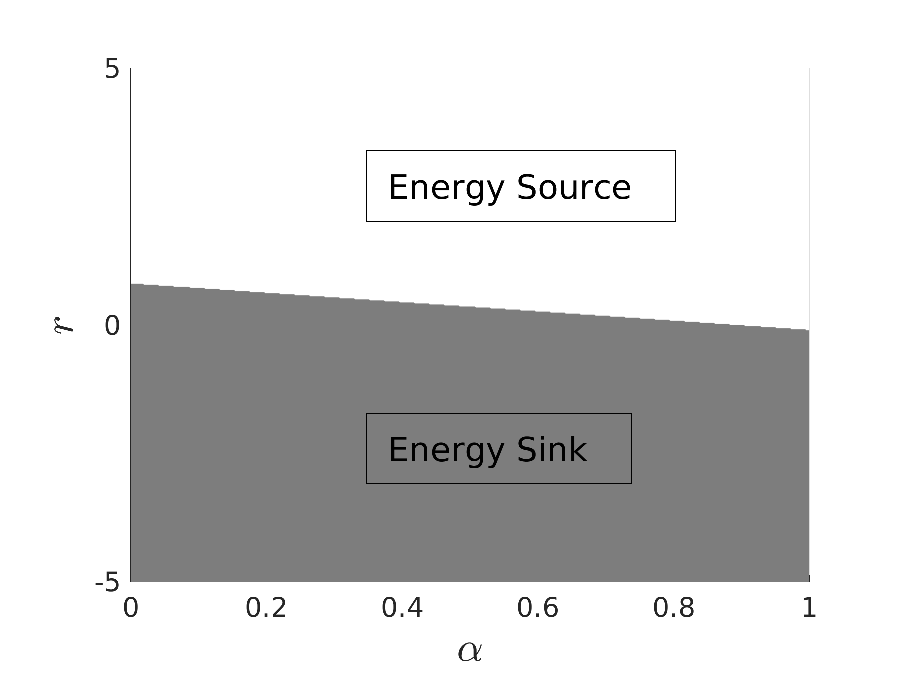
\includegraphics[width=3in]{filter_delta_energy}}
\caption{\small{Dissipative character of filtering for polynomial order $N=10$. Grey regions indicate the filter is dissipative while the white region indicates energy is being introduced into the flow by the filter.}}
\label{fig:filter_dissipation}
\end{figure}

The other aspect of the filtering operation which has been overlooked in the previous studies is its effect on the divergence-free condition. In order to asses the effects on divergence we revisit the double shear layer case studied in \cite{fischer01} and \cite{malm13}.

The flow case is setup in a two-dimensional domain $\Omega=[0,1]^{2}$ with doubly-periodic boundary conditions. The initial conditions are introduced as:
\begin{align}
 u_{0} &= 
 \begin{cases}
    	\tanh(\rho(y-0.25)),		& y \leq 0.5 \\
    	\tanh(\rho(0.75-y)),  	& y > 0.5
 \end{cases} \\
 v_{0} &= 0.05\sin(2\pi x),	\hspace{22pt}\forall\ x,y \nonumber
\end{align}
The domain is discretized with $16\times16$ spectral-element grid and each element uses $N=16$ Legendre polynomial modes, corresponding to $256$ points per element. The non-linear term is calculated using over-integration so as to preserve skew-symmetry of the advection term. The filtering stabilization procedure is also used to asses the effect of filtering on the divergence. $1\%$ of the last mode is filtered out at the end of each time-step. The tolerance of the solver for the divergence free condition is set to $10^{-10}$. Figure~\ref{fig:doubleshear_t0} shows the initial condition at time $t=0$ and Figure~\ref{fig:doubleshear_t2} shows the flow state at time $t=2$.

\begin{figure}[h]
	\centering
	\begin{subfigure}[b]{0.45\textwidth}
		\centering
		\includegraphics[width=1.1\columnwidth]{doubleshear_n16_t0}
		\caption{Initial vorticity at $t=0$}
		\label{fig:doubleshear_t0}
	\end{subfigure}
	\begin{subfigure}[b]{0.45\textwidth}
		\centering
		\includegraphics[width=1.1\columnwidth]{doubleshear_n16_t2}
		\caption{Vorticity at $t=2.0$}
		\label{fig:doubleshear_t2}
	\end{subfigure}
	\caption{Vorticity evolution for the double shear layer test case. }
	\label{fig:doubleshear_soln}
\end{figure}

Figure~\ref{fig:filter_divergence} shows the divergence of the flow field calculated before and after the application of the filter. The red line shows the divergence of the flow-filed after the pressure-correction step and the blue line indicates the divergence after the application of the filter. At the start of the simulation, when negligible energy is present in the last mode, the filter has very little impact on the divergence of the flow-field. However as the flow evolves and the energy in the smaller scales increase, violation of the divergence-free condition due to the action of the filter increases. This violation is substantial once the flow is fully developed, with the flow dropping nearly $6$ orders of magnitude in accuracy between the pressure-correction and the filtering step. This impact is surprisingly large. The case may be considered to be a stringent test with thin shear layers, which demand high resolution and thus even the small scales may contain dynamically significant energy. The situation however is representative of marginally resolved simulations where the smallest scales may still contain dynamically relevant energy, and thus filtering may have an unexpectedly large impact on the divergence-free condition of the flow-field.
\begin{figure}[h]
	\centerline{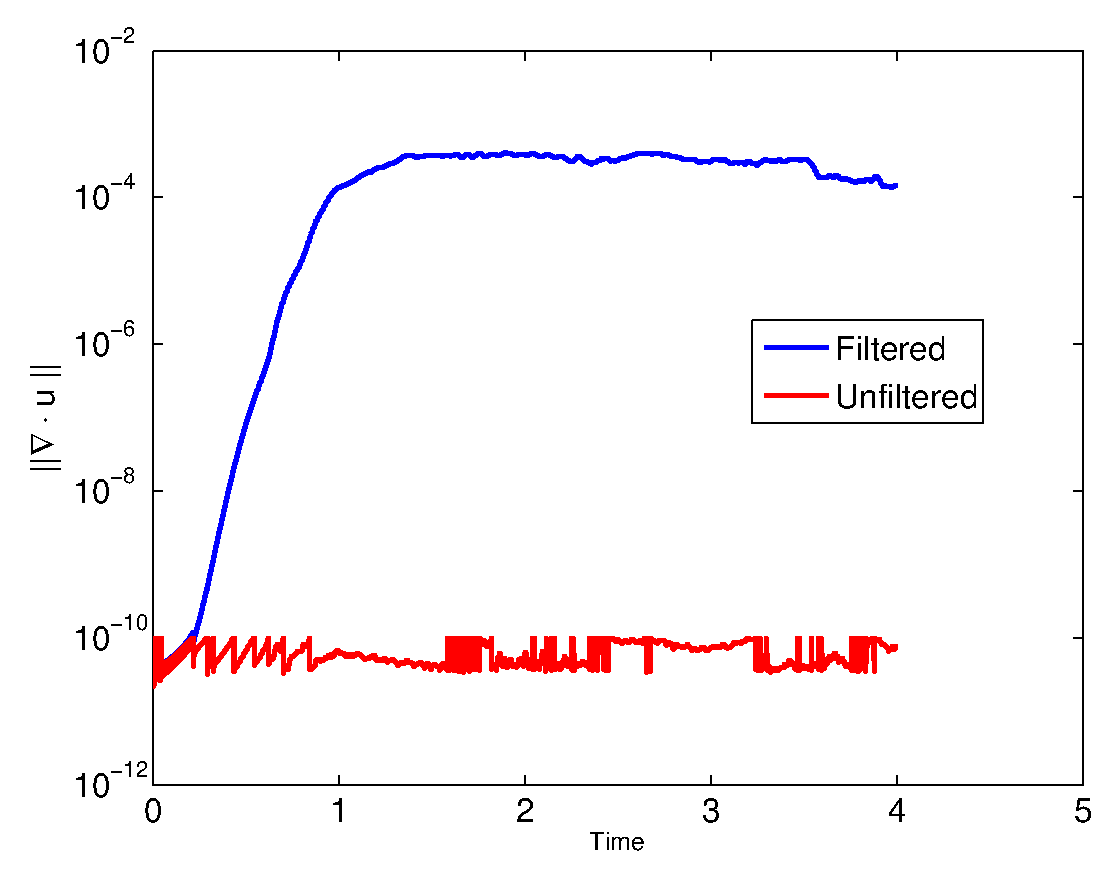
\includegraphics[width=3in]{divergence_filtered}}
	\caption{\small{The norm of the divergence after pressure correction and after filter application.}}
	\label{fig:filter_divergence}
\end{figure}

A puzzling aspect of the test as reported in the results of \cite{fischer01} and \cite{malm13} is that the case always needed some filter based stabilization. \cite{malm13} study the case with and without the use of over-integration for the non-linear term. They report that an order of magnitude lower filtering strength was needed when over-integration was used. However only over-integration did not ensure complete stabilization and the simulation experienced numerical instability at $T\sim6.7$ without filtering. \cite{malm13} attribute the destabilization to the finite accuracy of the divergence-free constraint, stating that even small errors would lead to numerical instability in the absence of dissipative terms (viscous or numerical) or stabilizing procedures (filtering). Although the authors do not report the tolerance to which the divergence free condition was satisfied. To check this again we run our test case with over-integration and without any filtering for a long duration. However contrary to the results obtained in \cite{malm13}, the simulation was stable (at least up to $T=20$). An explanation might be found when looking at the original test case reported in \cite{fischer01}. The authors there report using time steps such that the CFL number is between $1$ and $5$. The standard BDF3-K3 time-stepper would be unstable for these CFL numbers. This suggests that a characteristic time-stepping scheme may have been employed. We test the case by employing a the characteristic time-stepping scheme with over-integration but no filtering and indeed the simulation experienced numerical instabilities. This would implicate the characteristics time-stepper as the source of numerical instability. 

In retrospect, the results are to be expected. The use of consistent spaces for velocity and pressure avoids the spurious pressure oscillations. The absence of boundary conditions due to a doubly-periodic domain negates errors due to boundary terms, the use of over-integration dismisses aliasing errors as the source of instabilities and the spectral-element grid is perfectly Cartesian. Then as per the conclusion derived in \cite{malm13}, small divergence errors remain the obvious (known) source of numerical instability. However, these errors should be of the order of the specified solver tolerance for divergence. The (instantaneous) advection operator being real and skew-symmetric is a normal matrix (if evaluated completely using over-integration). Any violation of divergence-free condition of $O(\epsilon)$ can be regarded as a small perturbation to a normal matrix and one would expect a change in the eigenvalues to be of the same order $\epsilon$. Since in the ideal case the eigenvalues must lie on the imaginary axis with exactly zero real part, any perturbation due to numerical errors of order $O(\epsilon)$ would introduce new eigenvalues with a real part of $O(\epsilon)$. Thus a practical value for the solver tolerance of $10^{-8}$ would result in a advection matrix which would have eigenvalues with real parts of the order $10^{-8}$. Such a scenario creates an ever present numerical instability. However it should be an extremely weak instability, at least in such idealized test cases where other sources of instabilities are absent.

One can easily check the change of eigenvalues with varying degree of error in the advecting field. To do so we created a simple advection operator in Matlab following the spectral-element framework. A square domain with $\Omega=[0,1]^{2}$ is built and discretized using $3\times3$ spectral-elements which are further discretized using $10^{th}$ order Legendre polynomials. The advection operator is built on an over-integration grid with $19\times19$ grid points. The grid point spacing and weights for numerical integration correspond to the Gauss-Lobatto-Legendre points (GLL) for a polynomial of order $N_{d}=18$ resulting in the desired $18$ grid points for a complete integration of the convection term. Individual matrices are built independently for each spectral element and then a larger matrix for the whole system is built using direct stiffness summation. A simple sinusoidal divergence-free field can be used for building the $C\cdot\nabla$ matrix:
\begin{align}
\label{eqn:convection_op}
C_{x} &= 1.0 + 0.1\sin(2\pi x + 2\pi y) &+\epsilon\sin(2\pi x)\sin(2\pi y) \\
C_{y} &= 1.0 - 0.1\sin(2\pi x + 2\pi y) &+\epsilon\sin(2\pi x)\sin(2\pi y) \nonumber
\end{align}
When $\epsilon=0$ the field is analytically divergence free. Within the current numerical approximation the normalized divergence field defined as $||\nabla\cdot C|| = (\nabla\cdot C,\nabla\cdot C)/Volume$ is of the order $10^{-10}$. The parameter $\epsilon$ can thus be used to add a controlled perturbation to the advecting field and study the resulting change in eigenvalues. Figure~\ref{fig:spectra_eps0} and \ref{fig:spectra_eps-4} show the spectra of advection operator using $\epsilon=0$ and $\epsilon=10^{-4}$, resulting in divergence norms of the order $O(10^{-11})$ and $O(10^{-4})$ respectively. Tracking $\lambda_{max}$, defined as the eigenvalue with the largest real part, one can obtain how the instability of the advection operator changes with the variation of the divergence field. Figure~\ref{fig:lambda_dnorm} shows the change in $\lambda_{max}$ with $||\nabla\cdot C||$. As expected the trend is linear in a log-log scale with a slope of 1 across a variation of 8 orders of magnitude for $||\nabla\cdot C||$. This would suggest that relatively large divergence errors would be required for numerical instabilities to be caused by the advection term, as long as the term is evaluated completely. Of course as shown by \cite{malm13} and by \cite{kirby03}, the evaluation of this term without over-integration leads to instabilities in the absence of stabilization. These instabilities are much stronger than just divergence errors. Figure~\ref{fig:spectra_nodealias} shows the eigenvalue spectra for the advection operator (with $\epsilon=0$) evaluated on $11\times11$ GLL points in each element. The largest unstable eigenvalue is of the order $10^{-1}$, making the instability due to aliasing much stronger than the instabilities arising from the violation of the divergence-free condition.
\begin{figure}[h]
	\centering
	\begin{subfigure}[b]{0.45\textwidth}
		\centering
		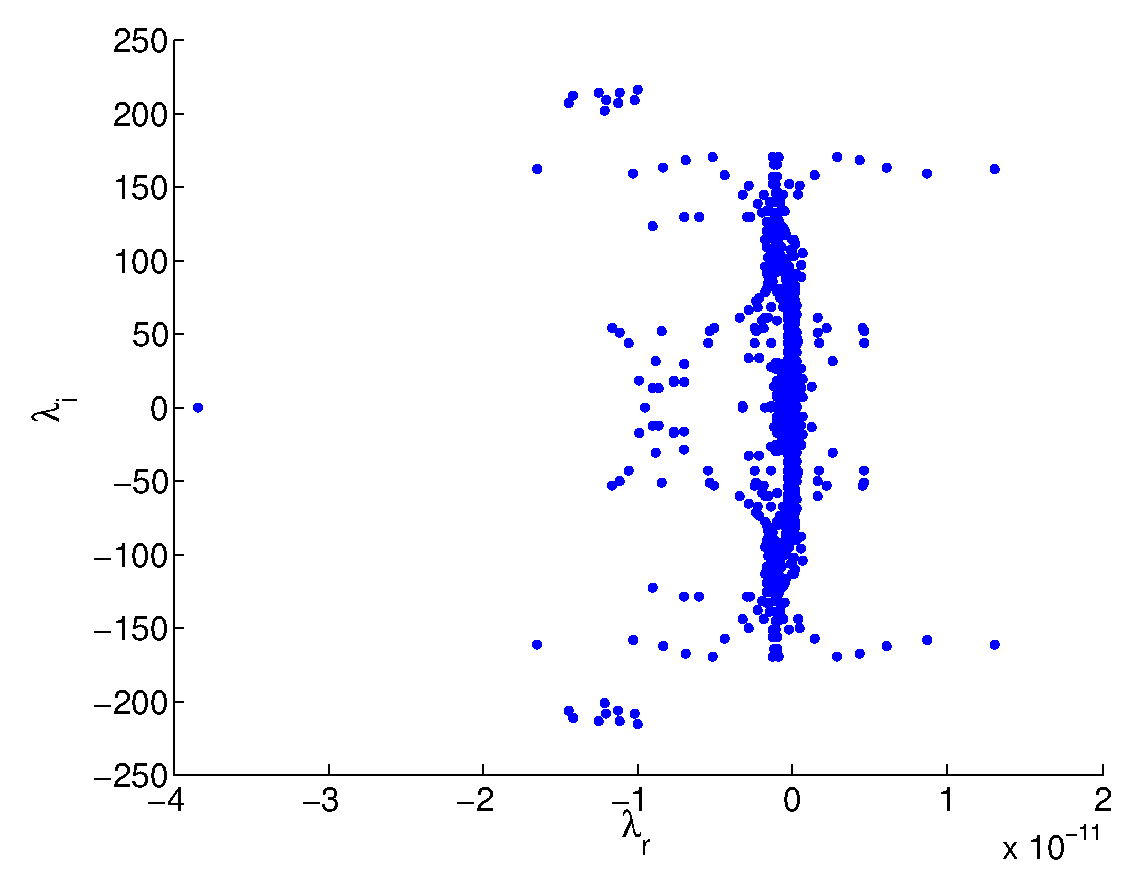
\includegraphics[width=1\columnwidth]{spectra_N10_Nxd18_nelv9_eps0}
		\caption{$||\nabla\cdot C|| \sim O(10^{-10})$}
		\label{fig:spectra_eps0}
	\end{subfigure}
	\begin{subfigure}[b]{0.45\textwidth}
		\centering
		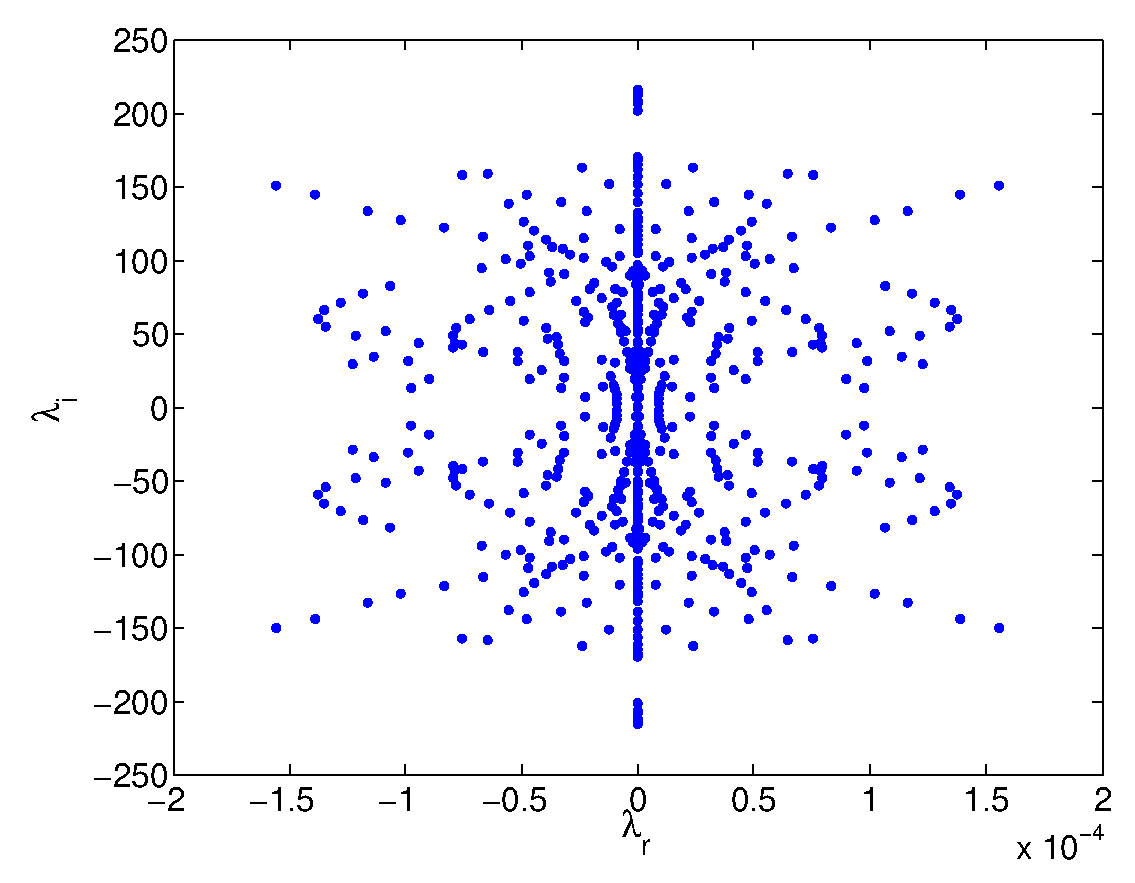
\includegraphics[width=1\columnwidth]{spectra_N10_Nxd18_nelv9_eps4}
		\caption{$||\nabla\cdot C|| \sim O(10^{-4})$}
		\label{fig:spectra_eps-4}
	\end{subfigure}
	\caption{Eigenvalue spectra for the advection operator with different divergence norms for a perturbed advecting field.}
	\label{fig:convection_spectra}
\end{figure}
\begin{figure}[h]
	\centerline{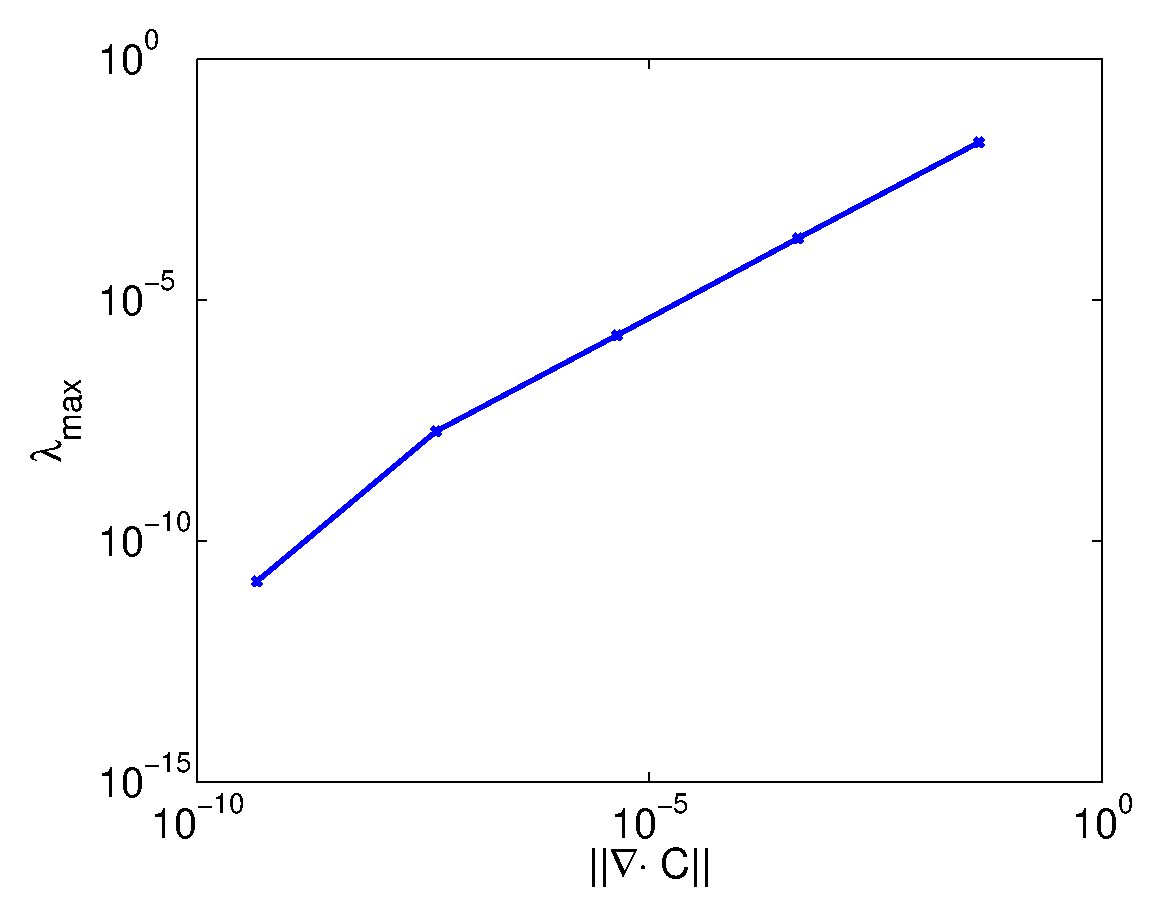
\includegraphics[width=2.5in]{N10_eig_dnorm}}
	\caption{\small{Variation of maximum real part of the eigenvalue spectrum with the norm of the divergence of the advection operator}}
	\label{fig:lambda_dnorm}
\end{figure}
\begin{figure}[h]
	\centerline{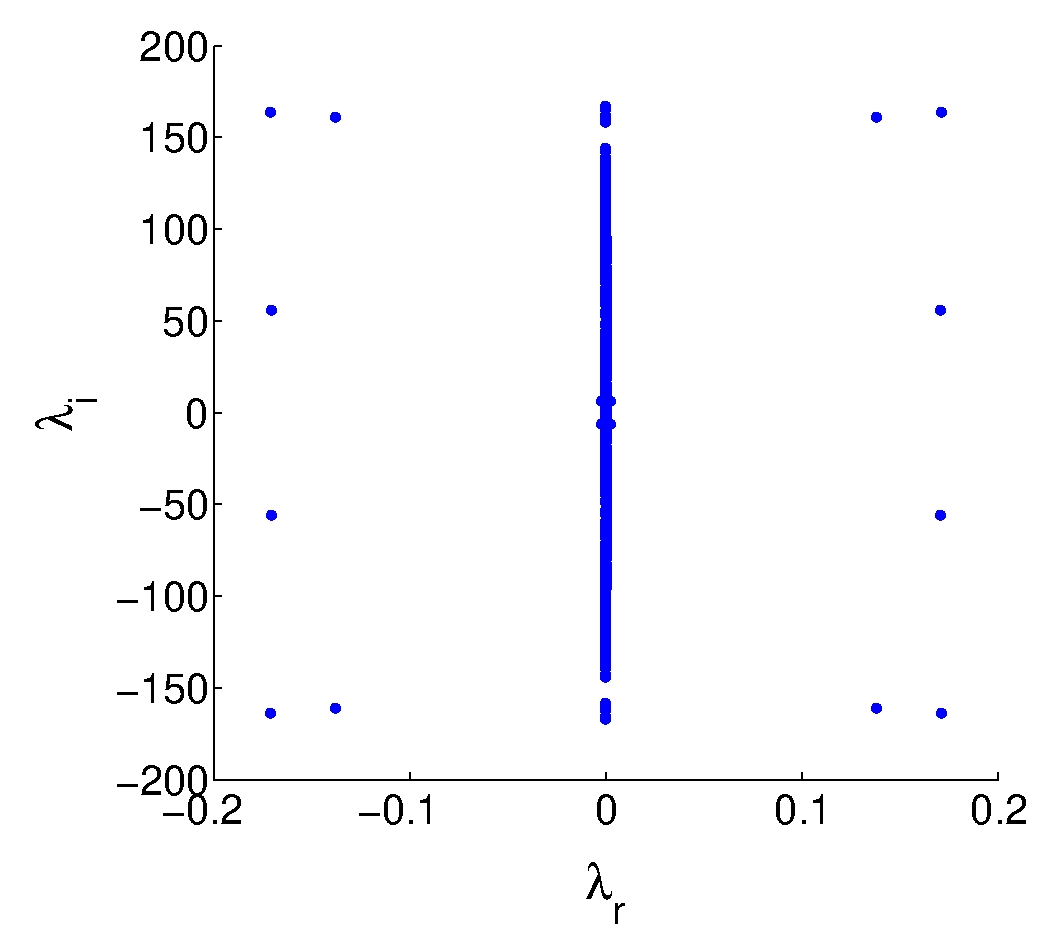
\includegraphics[width=2.5in]{spectra_nodealias_N10_Nd10}}
	\caption{\small{Eigenvalues for the advection term evaluated without over-integration}}
	\label{fig:spectra_nodealias}
\end{figure}
\cite{malm13} found that for the double shear layer case, the numerical instabilities first manifested in the thinnest part of the shear layers, thus concluding high shear regions necessarily need numerical stabilization. Since we do not experience any numerical instabilities using the BDF-EXT-k time stepping scheme, we further test this conclusion by reducing the resolution for the test case. We run the simulation with the same $16\times16$ spectral-elements but with polynomial orders of $N=11,7$ and $5$. These would lead to under-resolved shear layers. The under-resolution is strongly visible in the flow-field for the lowest polynomial order case of $N=5$. Figure~\ref{fig:vorticity_n6_t1} shows the vorticity in the flow field at time $t=1.0$ for $N=5$. However in all cases we find that the simulation does not experience any numerical instabilities (at least up till $t=20$) and additional stabilization was not required. The results indicate that in the absence of boundary terms and other sources of errors, under-resolution alone may not lead to numerical instabilities as long as the flow-field divergence remains small and the non-linear term is evaluated using complete over-integration. These results are consistent with those presented by \cite{kirby03} who found that they were able to simulate transition and turbulence in triangular ducts as well as turbulent channel flow simulations after employing over-integration but without additional flow stabilization.
\begin{figure}[h]
	\centering
	\includegraphics[width=3.5in]{doubleshear_n6_t1}
	\caption{\small{Vorticity at $t=1.0$ for the double shear layer case using polynomial order $N=5$}}
	\label{fig:vorticity_n6_t1}
\end{figure}


\section{Relaxation-term based stabilization}

In practical simulations over-integration errors may not be the only source of numerical instability and often it is found that simulations, especially those involving complex geometries or truncated domains require some amount to stabilization despite the use of over-integration. Filter-based stabilization has been an effective and efficient method to suppress such numerical instabilities. However the results of the previous section highlight some of the drawbacks of such a procedure. The loss of divergence free condition may be particularly severe for marginally resolved cases. In such a scenario, one may wish to look for an alternative method which preserves the advantages of explicit filtering, namely, efficiency and simplicity, while doing away with the potential drawbacks. One possible alternative in the context of the pressure-correction method is to perform the filtering procedure before the pressure-correction step. In the standard algorithm, the pressure-correction would follow a three-step procedure as follows: 
\begin{itemize}
	\item Velocity prediction $\rightarrow$ Pressure correction $\rightarrow$ Filtering.
\end{itemize}
A modified procedure would then follow:
\begin{itemize}
	\item Velocity prediction $\rightarrow$ Filtering $\rightarrow$ Pressure Correction.
\end{itemize}
This allows the filtering of the highest scales but leaves the solution unchanged after the divergence-free condition has been enforced. Such a procedure would remedy perhaps the most striking drawback of explicit filtering, which is the loss of divergence, while still retaining the simplicity and efficiency of explicit filtering operation. However the other drawbacks mentioned earlier, \textit{i.e} time-step dependence of filtered energy and the statistical nature of filter dissipation, still remain.

As it would turn out, there is an equally simple method that can resolve all the above mentioned deficiencies and is analogous to performing an explicit filtering procedure. As has been pointed out in \cite{stolz01} and \cite{schlatter04}, doing an explicit filtering operation is equivalent to doing an implicit time-relaxation. Formally, the two may be shown to be equivalent using a simple evolution equation \ref{eqn:NL_evolution}.
\begin{align}
\frac{\partial u}{\partial t} + \mathcal{F}(u) = 0
\label{eqn:NL_evolution}
\end{align}
Where $\mathcal{F}(u)$ is a (possibly non-linear) evolution operator.
The explicit filtering procedure may then be shown using a simple semi-discretized form of the evolution equation:
\begin{align}
u^{*} = u^{n} - \mathcal{F}(u^{n})\Delta t + O(\Delta t^{2})\nonumber \\
u^{n+1} =  \mathcal{G}(u^{*}) %& (\mathcal{G} - \text{Low pass filter.})
\label{eqn:NL_evolution_filtered}
\end{align}
Where $\mathcal{G}$ is a defined low-pass filter. As an alternate method, one may consider the same evolution equation supplemented by a relaxation-term as in equation~\ref{eqn:NL_evolution_rt}:
\begin{align}
\frac{\partial u}{\partial t} + \mathcal{F}(u) = \boldsymbol{-\chi \mathcal{H}(u)}
\label{eqn:NL_evolution_rt}
\end{align}
Which may be evolved using a time-splitting scheme:
\begin{align}
u^{*} = u^{n} -\mathcal{F}(u)\Delta t + O(\Delta t^{2})	\nonumber \\
u^{n+1} = u^{*} -\chi \mathcal{H}(u^{*})\Delta t + O(\Delta t^{2})
\label{eqn:NL_evolution_rt_1}
\end{align}
Taking the the parameter $\chi=1/\Delta t$ and $\mathcal{H}=\mathcal{(I-G)}$ to be the corresponding high-pass filter of $\mathcal{G}$, and substituting in equation \ref{eqn:NL_evolution_rt_1} one obtains:
\begin{align}
u^{n+1} = \mathcal{G}(u^{*}) + O(\Delta t^{2})
\label{eqn:NL_evolution_rt_2}
\end{align}
which is equivalent to the expression obtained in equation \ref{eqn:NL_evolution_filtered} to leading order of time discretization. \cite{stolz01} and \cite{schlatter04} interpret the relaxation-term as performing an equivalent low-pass filtering operation $\mathcal{G}$ every $1/(\chi\Delta t)$ time-steps. Alternately one may interpret this to mean that the relaxation-term procedure is equivalent to performing an explicit filtering operation with a filter strength of $(\chi\Delta t)$. 

Thus the ``filter-based stabilization'' operation proposed by \cite{fischer01} may be reformulated as an equivalent ``relaxation-term-based stabilization'', which we refer to as ``RT stabilization''. It can be easily incorporated into the Navier-Stokes by a simple addition of a relaxation-term on the right hand side. Thus the equivalent RT stabilized equation may be written as:
\begin{align}
\frac{\partial u}{\partial t} + u\cdot\nabla u = -\frac{\nabla p}{\rho} + \nu\nabla^{2}u -\chi\mathcal{H}(u) \\
\nabla\cdot u = 0
\label{eqn:rt_NS}
\end{align}
Where $\mathcal{H}(u)$ is a high-pass-filtered velocity field. The parameter $\chi$ may be used as a weighting parameter similar to the filter weight `$\alpha$' used in \cite{fischer01} and \cite{malm13}. Such a formulation immediately provides us with two advantages over the explicit filtering operation. Firstly, since there are no more explicit filtering operations after the pressure-correction step, the velocity field remains divergence free. Secondly, with the RT now part of the evolution equations, for a fixed $\chi$ and $\mathcal{H}$ the physical energy drain provided by the RT should be independent of the chosen time-step (as long as numerical stability is ensured). The final aspect of the stabilization concerning the dissipative character of the RT requires more constraints. When $\mathcal{H}$ is chosen to be positive semi-definite, and $\chi$ is a positive constant, the relaxation-term is purely dissipative. However with spatially varying $\chi$ and $\mathcal{H}$ the relaxation-term may be non-dissipative \citep{stolz03}.
\subsection{RT parameters}
\cite{malm13}, in the context of spectral-elements, describe a simple transfer function $\mathcal{G}$ defined for a variable in a one-dimensional domain $\Omega=[-1, 1]$ such that the filtering operation takes the simple form: 
\begin{align}
\bar{u}_{N}(x) = \mathcal{G}(u_{N}(x)) = \sum_{k=0}^{N}\sigma_{k}a_{k}\phi_{k}(x)
\end{align}
Where $\phi_{k}$ is the basis function and the definition of $\sigma_{k}$ describes the low-pass filter function $\mathcal{G}$ which takes the form:
\begin{align}
\sigma_{k} &=
	\begin{cases}
	1 - \alpha\left(\frac{k-k_{c}}{N-k_{c}}  \right)^{2}, & k>k_{c} \\
	1, & k\le k_{c}
	\end{cases}
\end{align}
Where $N$ is the number of modes in the spectral-element discretization and $k_{c}$ is the cut-off mode in spectral space used for building the filter. Amplitudes for modes $k\le k_{c}$ are unaffected by the filter operation. $\alpha$ is the filter weight such that $0\le\alpha\le1$. In keeping with our analysis earlier, we may define the corresponding high-pass filter $\mathcal{H}$ for the RT as:
\begin{align}
\mathcal{H}(u_{N}(x)) &= \sum_{k=0}^{N}\gamma_{k}a_{k}\phi_{k}(x) \\
\gamma_{k} &=
\begin{cases}
	\left(\frac{k-k_{c}}{N-k_{c}}  \right)^{2}, & k>k_{c} \\
	0, & k\le k_{c}
\end{cases}
\end{align}
Where the parameter $\alpha$ is absorbed into $\chi$ which acts as an RT strength term. To formally have the same operation as the explicit filter, the value of $\chi$ can be set to $\chi=(\alpha/\Delta t)$. This is in agreement with our earlier interpretation that the RT procedure is equivalent to performing a low-pass filter operation every time-step with a strength of $(\chi\Delta t)$. Using this value we get $\chi\Delta t = \alpha$ and thus we recover the correct weighting for the equivalent explicit filter operation. 

The basis functions $\phi$ used for the definition of $\mathcal{H}$ however is different from the one used by \cite{malm13} who use the transformed basis functions described by \cite{boyd98} which are described in equation~\ref{eqn:boyd}. Using this basis function however, the form of $\mathcal{H}$ is not semi-positive definite and thus the relaxation term is not purely dissipative. This is rather expected from our earlier results which show that the explicit filter operation using such a transformed basis has a substantial parameter range where it acts as an energy source. The equivalent RT formulation then can not be purely dissipative. We use the Legendre polynomials as the basis functions (for a Legendre-spectral-element method) for building the RT which makes $\mathcal{H}$ semi-positive definite. Thus for $\chi>0$ the relaxation term $-\chi\mathcal{H}(u)$ is always purely dissipative.

\subsection{Stability and parameter range}
The action of the RT can be inferred from the change in eigenvalues of the system due to the added stabilization. As an illustration we build the system matrices using the simple $3\times3$ spectral-element grid in Matlab for a linear advection operator stabilized by a relaxation-term. The advection operator is built using the parameters in equation~\ref{eqn:convection_op}. We set $\epsilon=10^{-2}$ so that the operator now models a numerically unstable system with positive eigenvalues. The eigenvalues of the unstable system without the addition of a relaxation term are shown in figure~\ref{fig:spectra_conv_eps2}. As expected, there are unstable eigenvalues with positive real part of order $O(10^{-2})$. With the addition of an RT as defined earlier, with $k_{c}=10$ and $\chi=0.4$ causes the eigenvalues to shift towards the negative real plane (figure~\ref{fig:spectra_rhs_eps2}). In the example shown here, the instability appears to be completely suppressed and the largest real part of the eigenvalues of the resulting system is zero. The overall system is more dissipative as evidenced by the general negative shift of the real part of the eigenvalues.
\begin{figure}[h]
	\centering
	\begin{subfigure}[b]{0.45\textwidth}
		\centering
		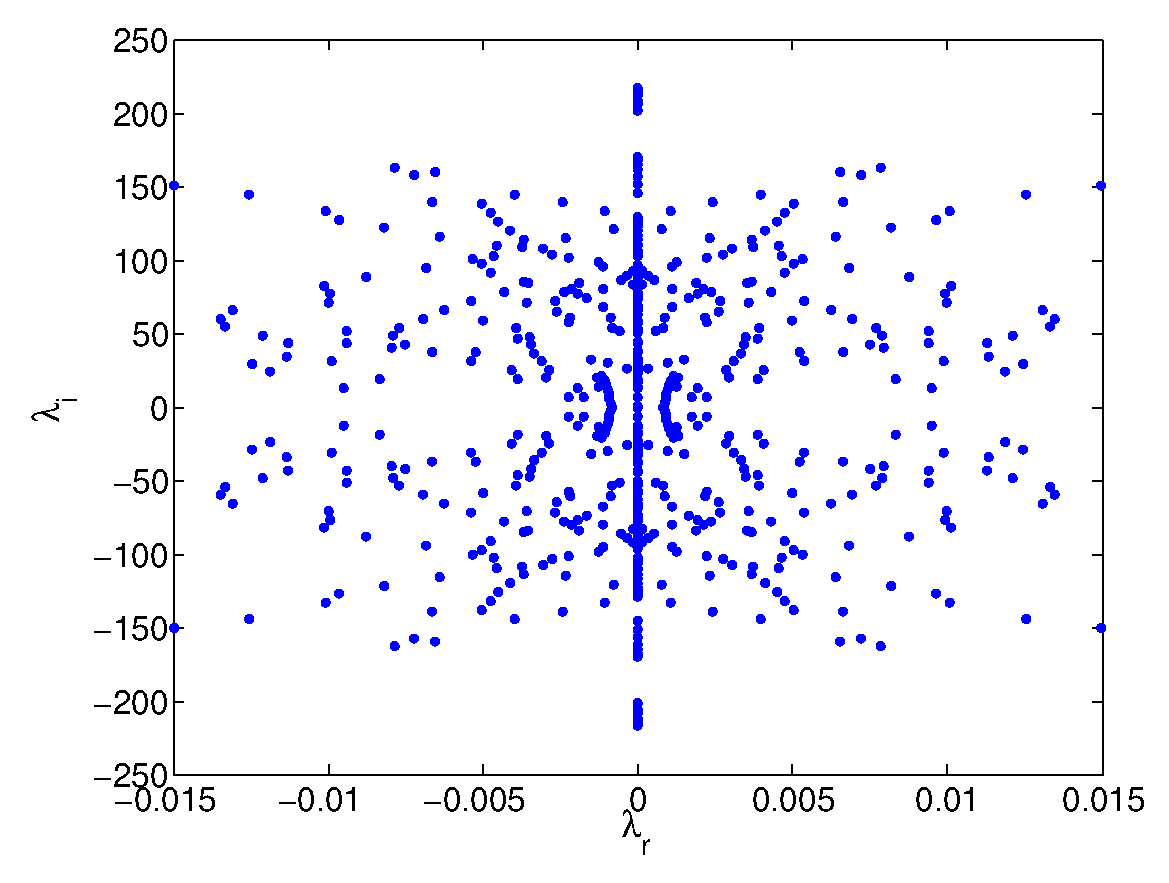
\includegraphics[width=1\columnwidth]{spectra_conv_N10_Nxd18_nelv9_eps2}
		\caption{$||\nabla\cdot C|| \sim O(10^{-2})$}
		\label{fig:spectra_conv_eps2}
	\end{subfigure}
	\begin{subfigure}[b]{0.45\textwidth}
		\centering
		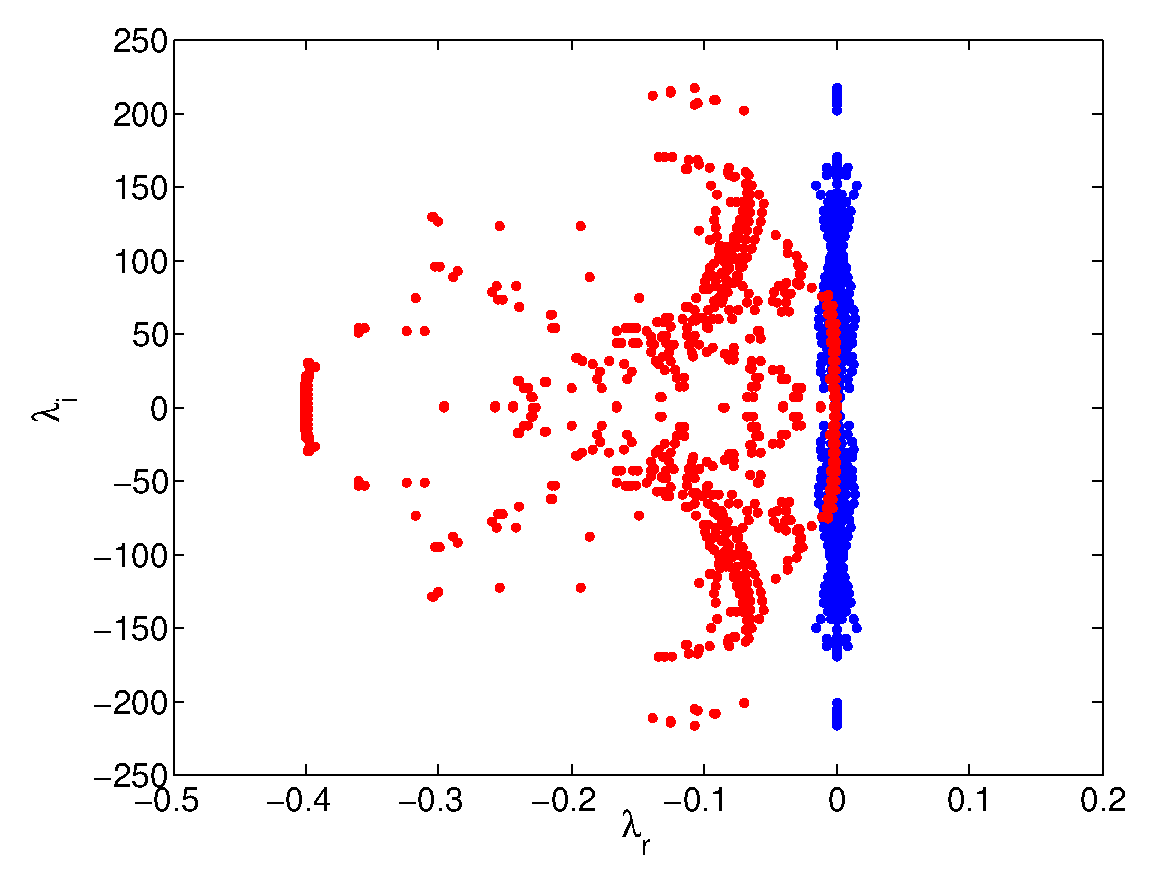
\includegraphics[width=1\columnwidth]{spectra_rhs_N10_Nxd18_nelv9_eps2}
		\caption{Stabilized Eigenvalues.}
		\label{fig:spectra_rhs_eps2}
	\end{subfigure}
	\caption{Comparison of eigenvalues for an unstable system (a) with $||\nabla\cdot C|| \sim O(10^{-2})$ and a system stabilized using a relaxation-term (b)}
	\label{fig:rt_spectra}
\end{figure}

While the RT clearly has a stabilizing effect on the system, it can also be destabilizing for a certain range of parameters. From figure~\ref{fig:spectra_rhs_eps2} one can notice some eigenvalues of the stabilized system have a large negative shift with the smallest real part being $\lambda_{r}^{min}=-0.4$. As it turns out this particular eigenvalue sets the stability limits of the RT stabilization approach. For a particular temporal discretization such as the BDF-EXT-3, the region of stability may cover a finite region of the negative plane. For a system with eigenvalues such that $\lambda\Delta t$ falls outside the stability region of the time-stepping scheme, the system becomes numerically unstable. The scaled eigenvalues with varying values of the parameter $\chi\Delta t$ (and $k_{c}=1$) are shown in figure~\ref{fig:rt_stability} with a black line enveloping the region of stability for a BDF-EXT-3 temporal discretization scheme. As the strength of the RT stabilization is increased by varying $\chi$, the eigenvalues become more negative and the dissipative character of the stabilization procedure becomes stronger. Eventually as $\chi\Delta \approx 1$ the stabilization procedure itself becomes numerically unstable and the time-step needs to be reduced in order to render the simulation numerically stable again. The analysis is exemplified using the BDF-EXT-3 scheme but the concept generalizes to other schemes and the limit of stability will be governed by the stability region of the respective schemes.
\begin{figure}[h]
	\centering
	\begin{subfigure}[b]{0.45\textwidth}
		\centering
		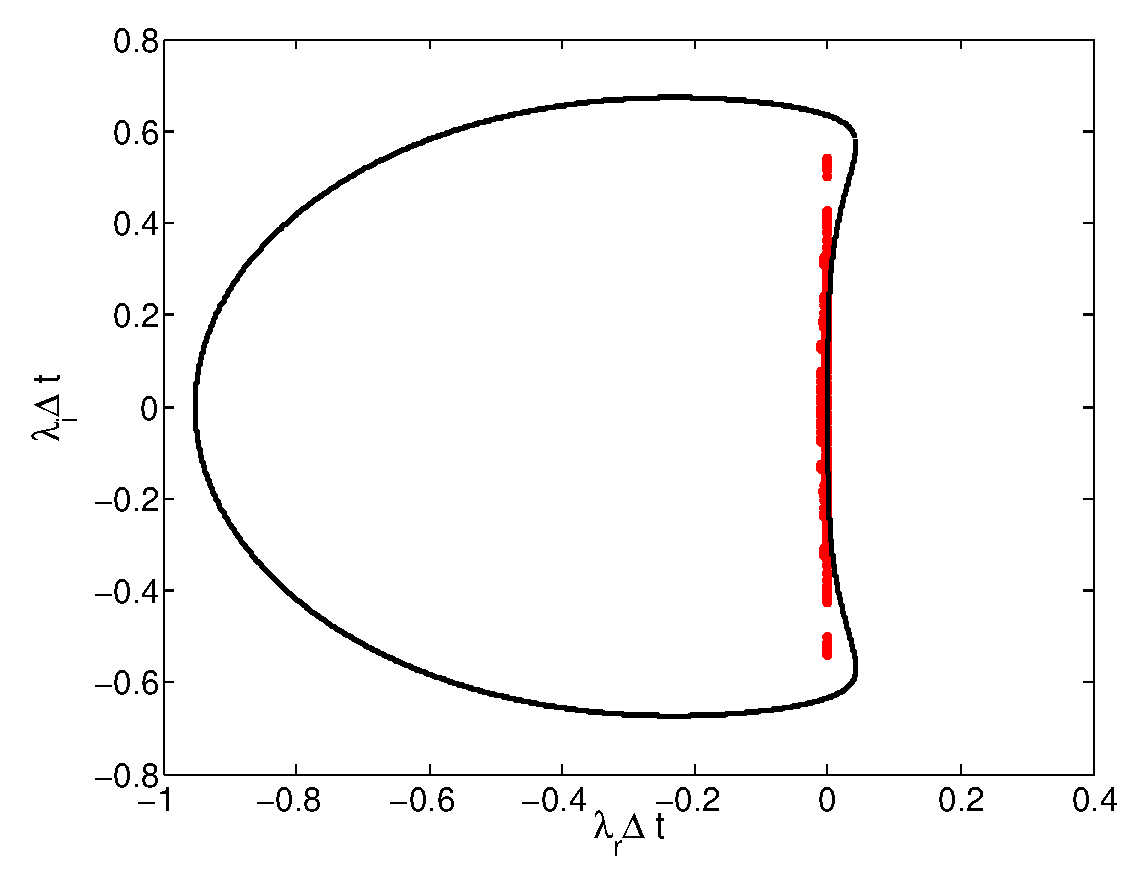
\includegraphics[width=1\columnwidth]{spectra_chidt_001}
		\caption{$\chi\Delta t=0.01$}
		\label{fig:spectra_chidt001}
	\end{subfigure}
	\begin{subfigure}[b]{0.45\textwidth}
		\centering
		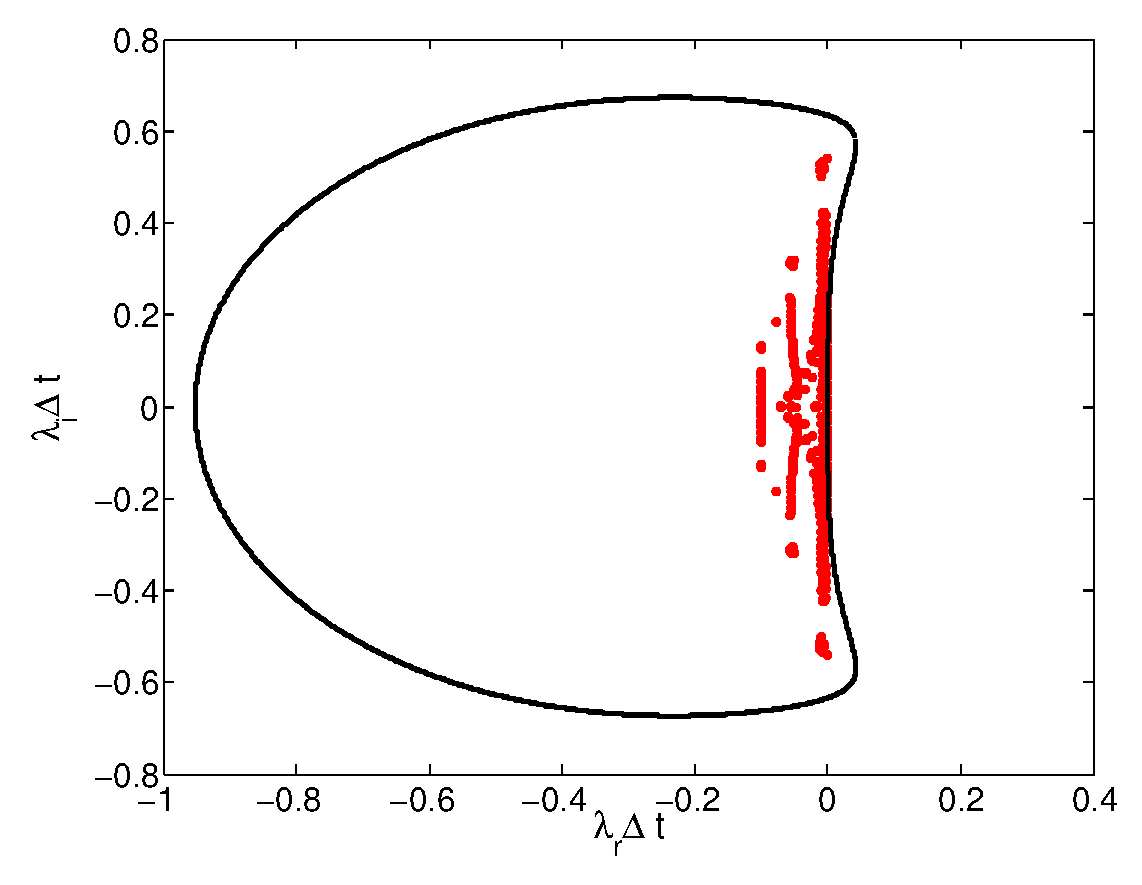
\includegraphics[width=1\columnwidth]{spectra_chidt_010}
		\caption{$\chi\Delta t=0.10$}
		\label{fig:spectra_chidt01}
	\end{subfigure}
	\begin{subfigure}[b]{0.45\textwidth}
		\centering
		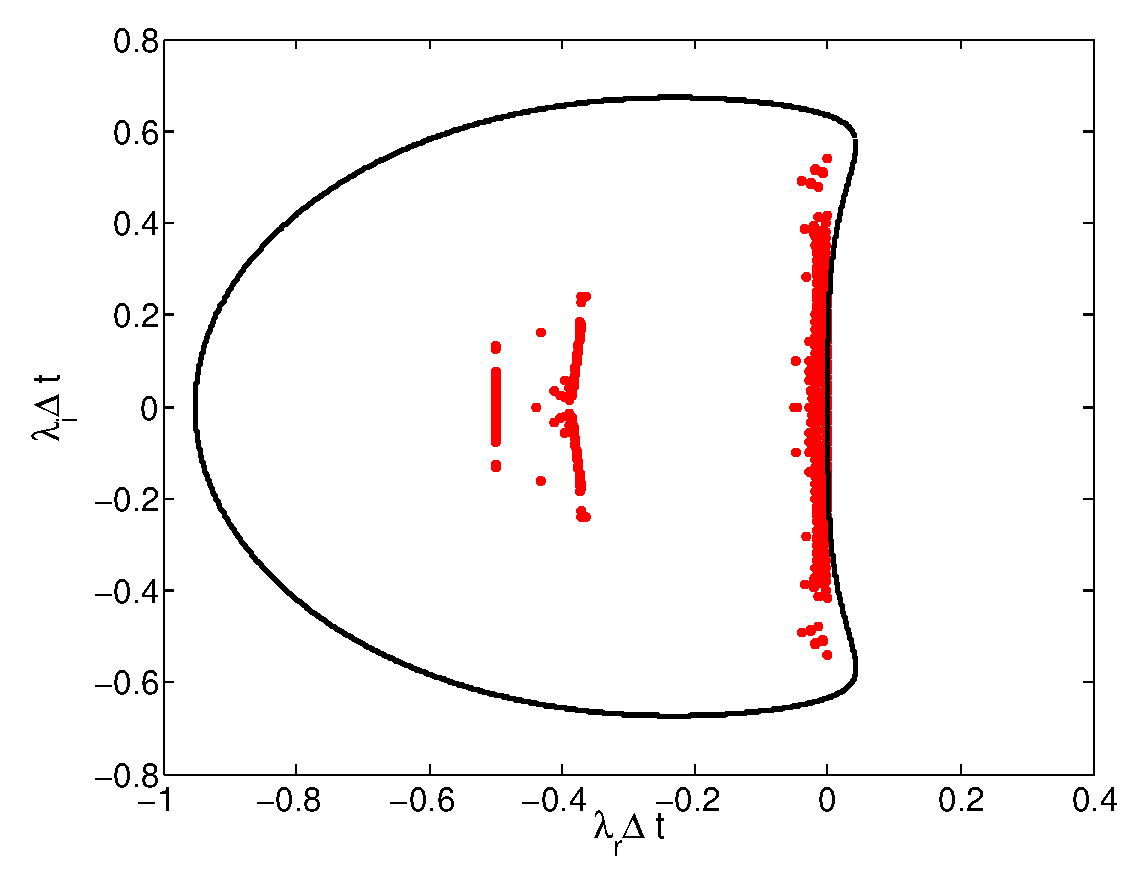
\includegraphics[width=1\columnwidth]{spectra_chidt_050}
		\caption{$\chi\Delta t=0.50$}
		\label{fig:spectra_chidt050}
	\end{subfigure}
	\begin{subfigure}[b]{0.45\textwidth}
		\centering
		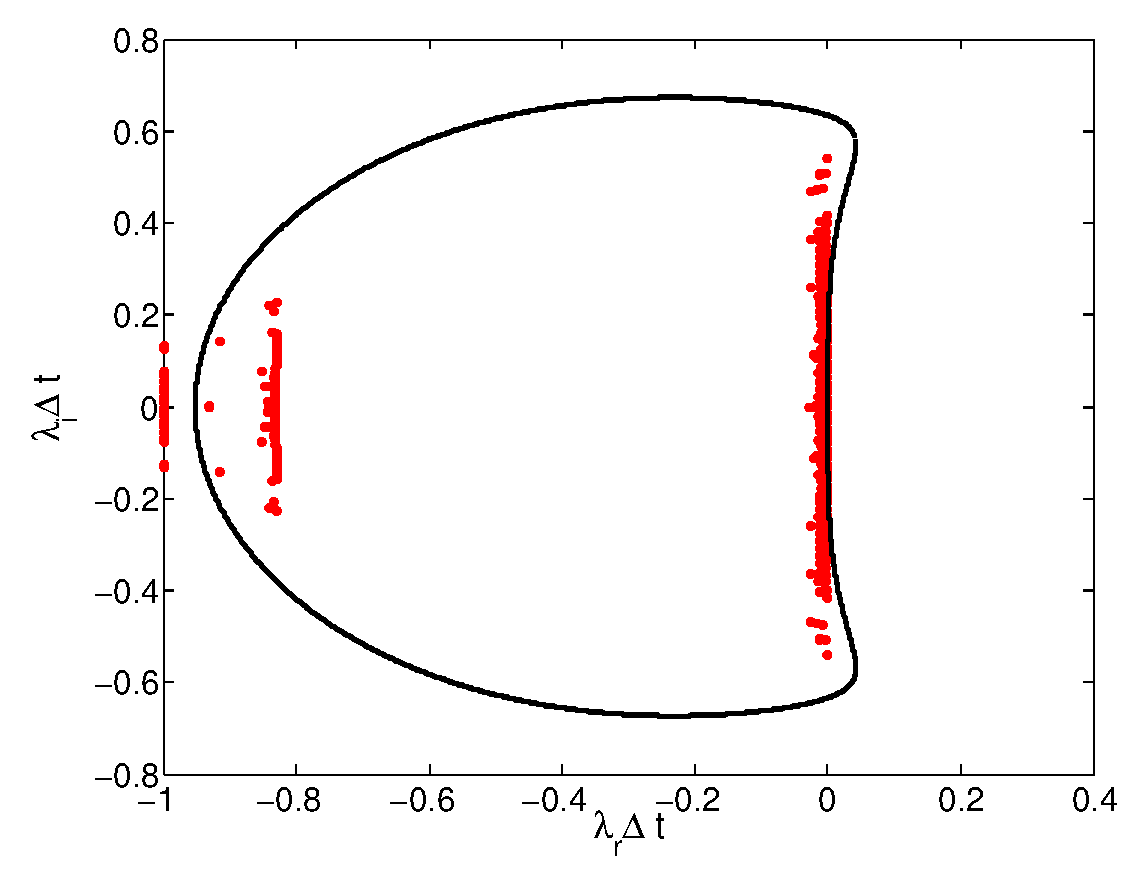
\includegraphics[width=1\columnwidth]{spectra_chidt_100}
		\caption{$\chi\Delta t=1.00$}
		\label{fig:spectra_chidt100}
	\end{subfigure}	
	\caption{Changes in eigenvalues with varying filter strength $\chi\Delta t$ with $k_{c}=10$.}
	\label{fig:rt_stability}
\end{figure}
This condition limits the parameter range for which a relaxation-term type stabilization can be used. Practical values of the $\chi$ parameter should not reach such a limit. To compare with an explicit filtering case, practical values of the filter strength vary between $0\le\alpha\le0.3$ which correspond to $0\le\chi\Delta t\le0.3$. \cite{fischer01} apply the filtering procedure with $\alpha=1.0$ and note that lower values of $\alpha$ are preferable. Should one find that the dissipation provided at low values of $\chi$ is not enough, the alternative would be to change the cut-off wavenumber $k_{c}$. This increases the added dissipation by the relaxation-term but does not substantially change the stability limits. Figure~\ref{fig:rt_stability_k8} shows the change in eigenvalues with different $\chi\Delta t$ using the cut-off mode number as $k_{c}=8$. The system is clearly more dissipative with many more eigenvalues with large negative real parts. However the approach to numerical instability remains approximately the same at $\chi\Delta t\approx 1.0$.
\begin{figure}[h]
	\centering
	\begin{subfigure}[b]{0.45\textwidth}
		\centering
		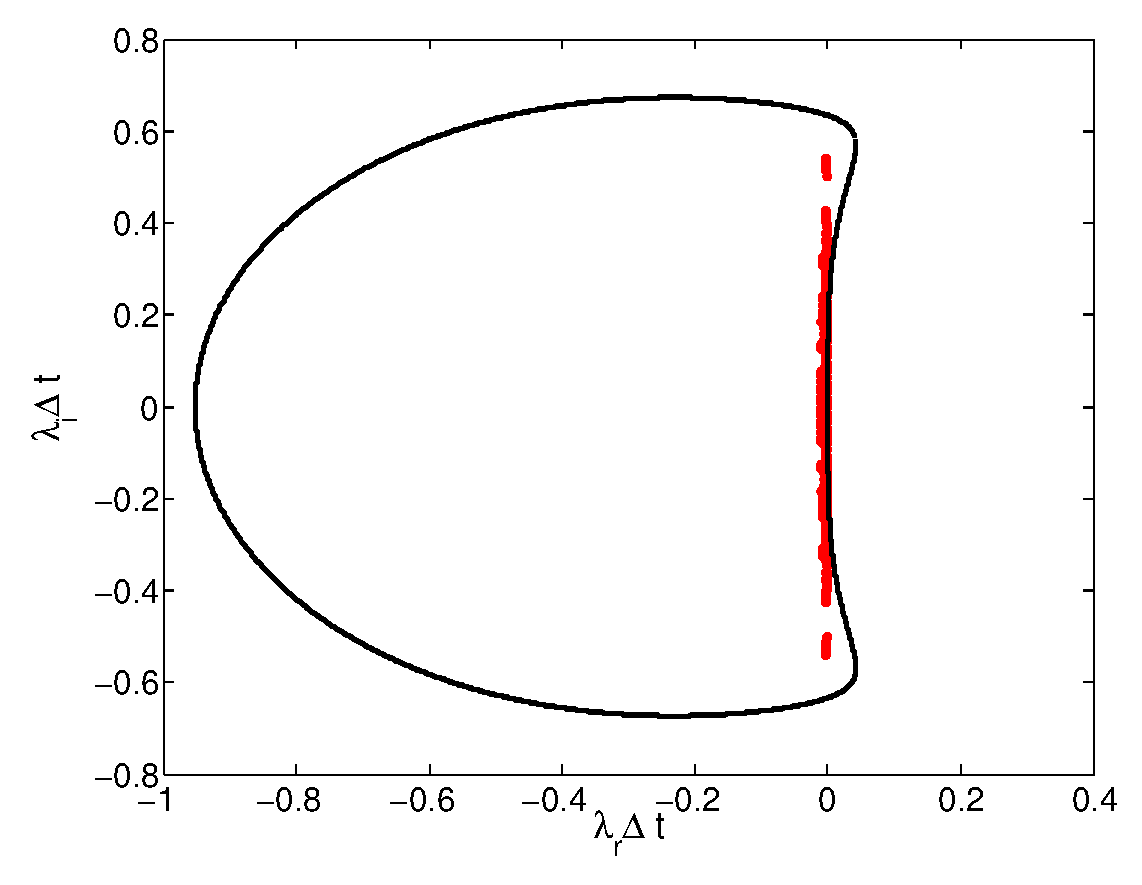
\includegraphics[width=1\columnwidth]{spectra_chidt_001_k8}
		\caption{$\chi\Delta t=0.01$}
		\label{fig:spectra_chidt001_k8}
	\end{subfigure}
	\begin{subfigure}[b]{0.45\textwidth}
		\centering
		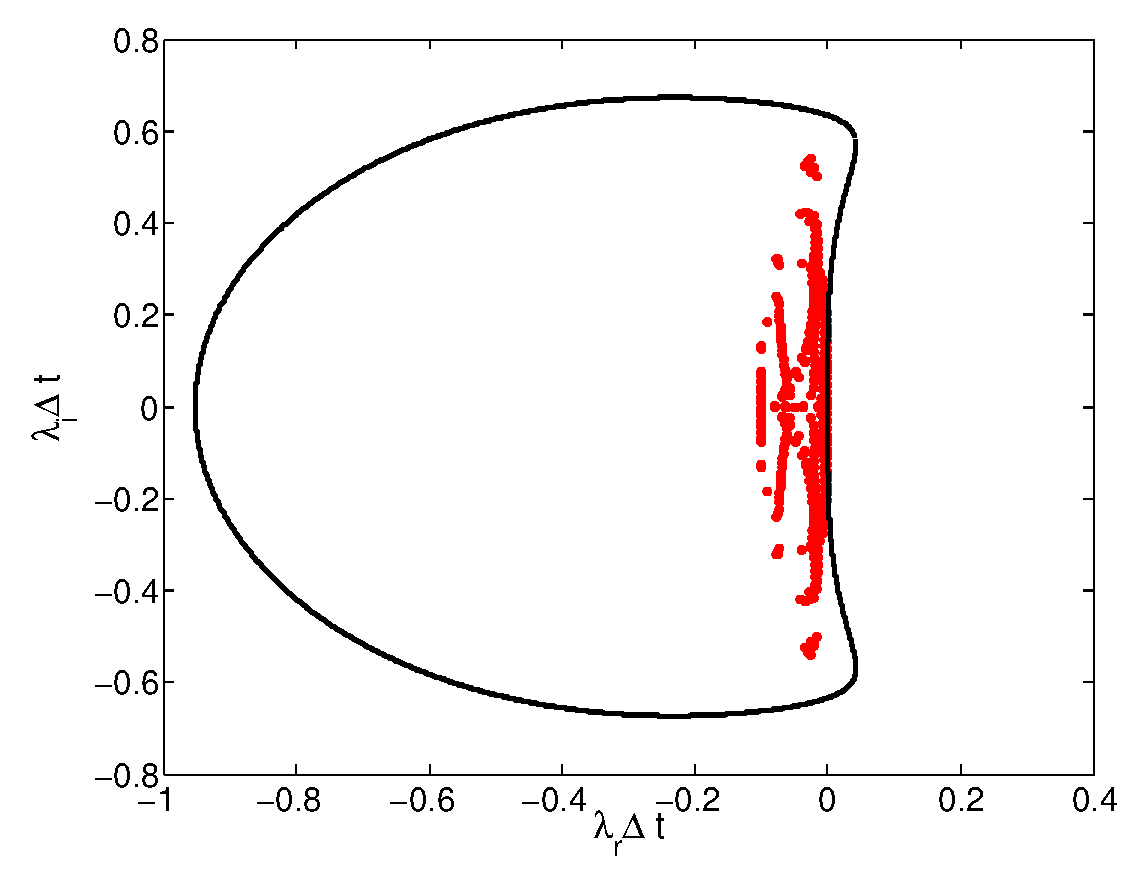
\includegraphics[width=1\columnwidth]{spectra_chidt_010_k8}
		\caption{$\chi\Delta t=0.10$}
		\label{fig:spectra_chidt01_k8}
	\end{subfigure}
	\begin{subfigure}[b]{0.45\textwidth}
		\centering
		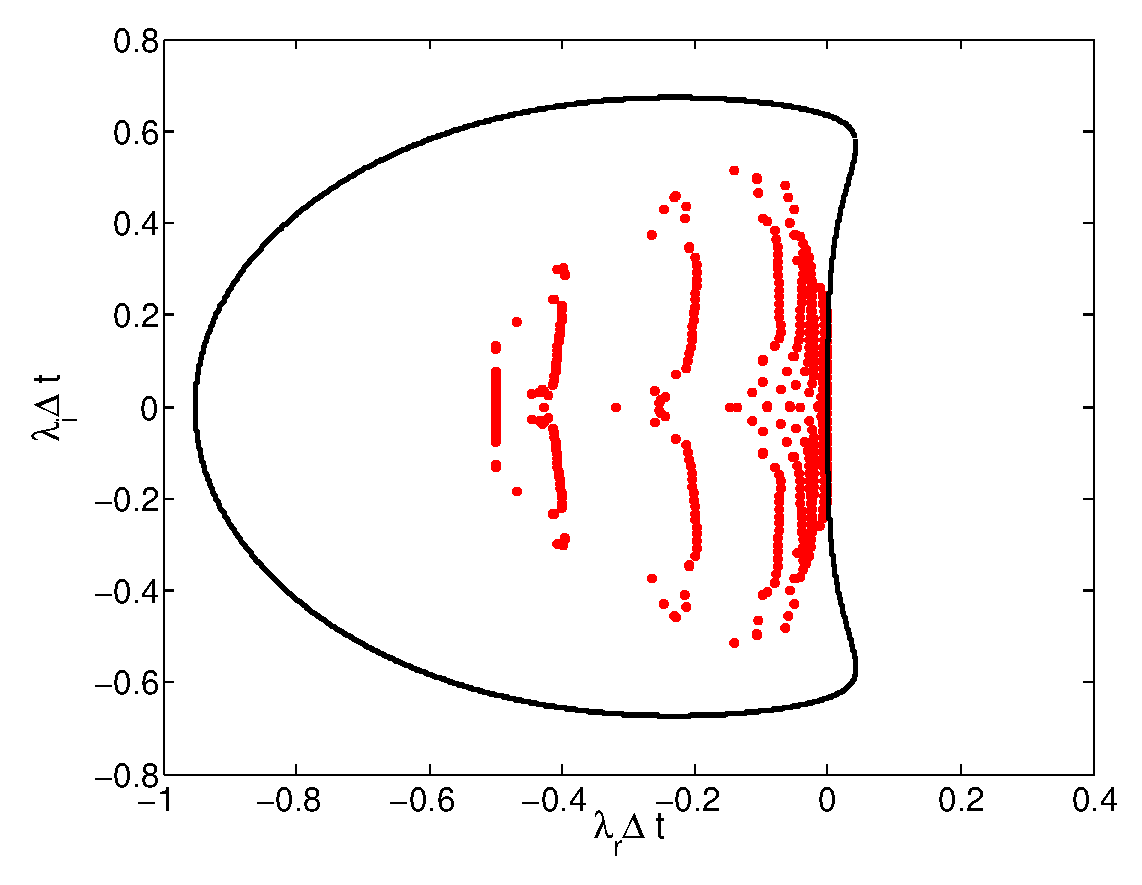
\includegraphics[width=1\columnwidth]{spectra_chidt_050_k8}
		\caption{$\chi\Delta t=0.50$}
		\label{fig:spectra_chidt050_k8}
	\end{subfigure}
	\begin{subfigure}[b]{0.45\textwidth}
		\centering
		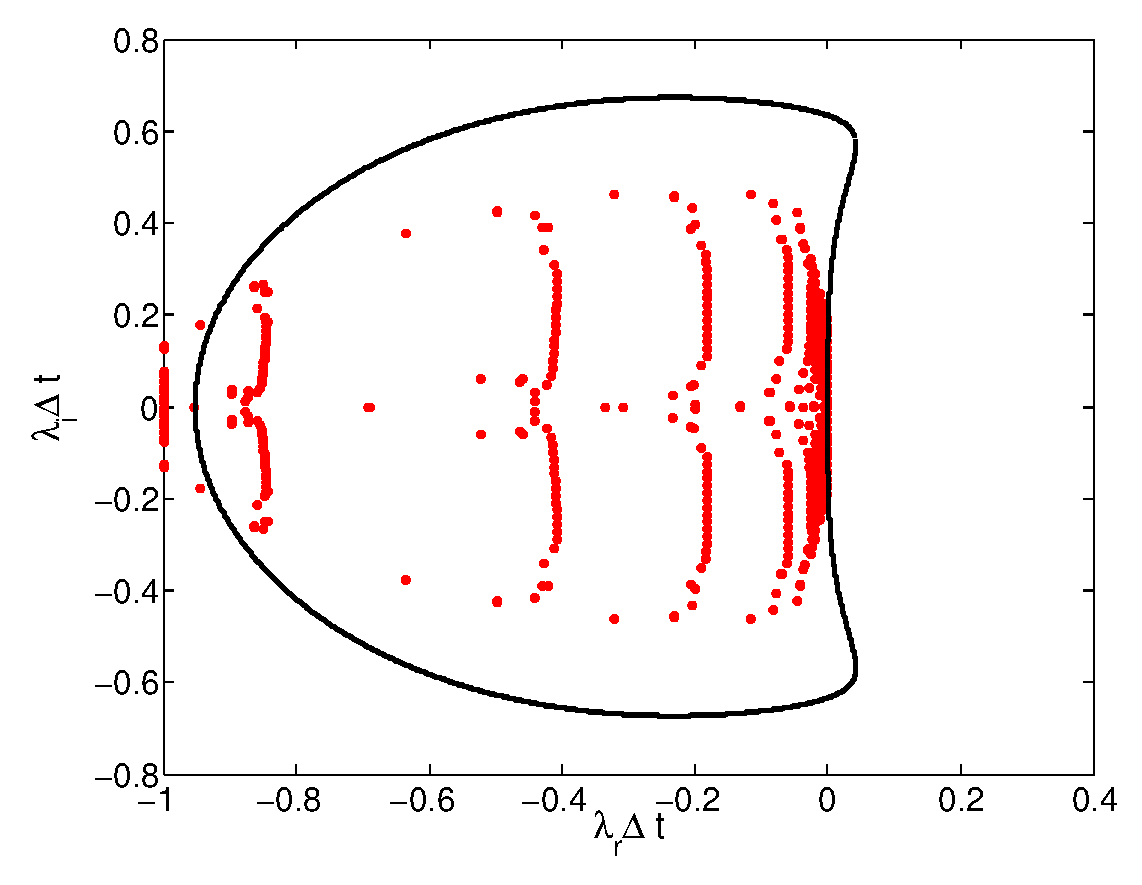
\includegraphics[width=1\columnwidth]{spectra_chidt_100_k8}
		\caption{$\chi\Delta t=1.00$}
		\label{fig:spectra_chidt100_k8}
	\end{subfigure}	
	\caption{Changes in eigenvalues with varying filter strength $\chi\Delta t$ with $k_{c}=8$.}
	\label{fig:rt_stability_k8}
\end{figure}

It is important to note that such a formulation is very similar to the RT-3D approach used by \cite{schlatter04} in the context of large-eddy simulations of transitional flows. In the study the authors compare different variants of the ADM-RT (approximate deconvolution model with relaxation term) for transitional and turbulent regimes. In the RT-3D variant the non-linear terms are computed without the deconvolution procedure and hence only the relaxation-term is used for modeling the sub-grid stresses. In the current study we are only concerned with the relaxation-term procedure in the context of numerical stabilization. 

\subsection{Double shear layer}
We test the RT stabilization in the 2D model test case of double shear layer as done in by \cite{fischer01} and \cite{malm13} for a several different parameters. Quite expectedly the procedure successfully stabilizes the simulations. We show the results of only one test case when no over-integration is employed, which would be the most stringent test case for stabilization. We ran the test using a $16\times16$ spectral-element grid with $N=16$ Legendre modes in each spectral-element. The RT parameters of $\chi=1.5\times10^{-3}$ (corresponding to $\chi\Delta t=0.3$) and $k_{c}=15$ were used. Figure~\ref{fig:rt_n15_t2} shows the vorticity in the field at $t=2.0$ where the thin shear layers are clearly visible. The simulation ran without numerical instabilities up to $t=20$.
\begin{figure}[h]
	\centering
	\includegraphics[width=3.0in]{visit_rt_t2}
	\caption{\small{Vorticity at $t=2.0$ for the double shear layer case using polynomial order $N=16$ without over-integration and using a relaxation-term stabilization.}}
	\label{fig:rt_n15_t2}
\end{figure}


\section{Conclusion}
We reassess the filter-based stabilization proposed by \cite{fischer01} and find that despite its appealing simplicity and efficiency, it suffers from several drawbacks, the most striking of which is the loss of the divergence-free condition of the flow field. In marginally resolved simulations, this loss may be severe as in our model test case where 6 orders of accuracy was lost for the divergence-free condition. Two other drawbacks are the time-step dependence of the filtered energy and the statistical character of the filter dissipation. An alternate formulation for stabilization is proposed called the ``relaxation-term-based stabilization'' or RT stabilization, which is closely related to the explicit filtering operation. With appropriate parameters can be shown to be equivalent to an explicit filter operation to leading order of time discretization. The procedure stabilizes the numerical method without destroying the divergence-free condition and for an appropriately built high-pass filter $\mathcal{H}$ the term has the quality of being purely dissipative. Moreover, the stabilization is now part of the evolution equations, and thus the energy drain due to relaxation-term is independent of the chosen time-step. Limits of the stabilization are also shown and under certain parameters the stabilization itself becomes numerically unstable. However the procedure is stable under the standard parameter ranges which may be expected for numerical stabilization. Test cases with the double shear layer shows the relaxation-term is able to stabilize the numerical simulation even in the absence of over-integration, which corresponds to a fairly stringent case of numerical stability in the presence of negligible viscosity.




%\begin{footnotesize}
%\bibliography{licentiate}\bibliographystyle{jfm}
%\end{footnotesize}

%\end{document}



%------------------------------------------------------------------------------
% Bibliography
%------------------------------------------------------------------------------
%
%\clearpage
\bibliographystyle{jfm}
\bibliography{licentiate}
%
%\IfFileExists{stabilization/paper.bbl}{%------------------------------------------------------------------------------
% Define title, author(s), affiliation and publishing status
%
\papertitle[Rexalation-term stabilization] % Short title used in headlines (optional)
{%
  A re-examination of filter-based stabilization for spectral element methods% THE COMMENT SYMBOL AT THE END OF THIS LINE IS NEEDED
}%
%
\papertoctitle{Relaxation-term-based stabilization} % Title for toc
%
\paperauthor[Negi P. S.] % Short authors used in headlines and List Of Papers
{%
  P. S. Negi %$^{1,2}$, P. Schlatter$^{1,2}$, A. Hanifi$^{1}$ and D. S. Henningson$^{1,2}$%
}%
%
%\listpaperauthor{A. Skywalker \& D. Vader}% (optional) Short authors used in List Of Papers
%
\paperaffiliation
{%
%  $^1$ Linn\'e FLOW Centre, KTH Mechanics, S-100 44 Stockholm, Sweden\\
%  $^2$ Swedish e-Science Research Centre (SeRC), SE-100 44, Stockholm, Sweden%
  Linn\'e FLOW Centre, KTH Mechanics, S-100 44 Stockholm, Sweden\\
  Swedish e-Science Research Centre (SeRC), SE-100 44, Stockholm, Sweden%
}%
%
\paperjournal[Gal. Empire Publ.] % Short publish info used in List Of Papers
{%
	Galactic Empire Publications%
}%
%
\papervolume{42}%
%
\papernumber{2}%
%
\paperpages{1--10}%
%
\paperyear{3639}%
%
\papersummary%
{% Insert summary of the paper here (used in introduction) 
	The implications of concurrent archetypes have been far-reaching and
	pervasive. Given the current status of heterogeneous technology,
	cyberinformaticians daringly desire the key unification of the Turing
	machine and erasure coding. We explore new decentralized information,
	which we call Tuna.
}%
%
\graphicspath{{stabilization/imgs/}}%
%
%
%===============================================================================
%                            BEGIN PAPER
%===============================================================================
%
\begin{paper}

\makepapertitle

%------------------------------------------------------------------------------
% Abstract
%------------------------------------------------------------------------------
%
\begin{paperabstract}
	We revisit the ``filter-based stabilization'' approach proposed by \cite{fischer01} and find that it suffers from several drawbacks. In particular the ``evolve and filter'' approach causes a violation of the divergence-free condition which can be particularly severe in the cases of marginally resolved flows. Moreover the form of the filtering operation causes the filter to not be purely dissipative. Instead of a filter-based approach we propose to use a ``relaxation-term-based stabilization'' which we refer to as an RT stabilization, which is very closely related to the explicit filtering operation. The method retains the advantages of simplicity and efficiency of a filter based approach while also remedying the above mentioned drawbacks. Parameter limits of such a stabilization procedure are explored and the method is shown to be effective within the practical parameter ranges.
\end{paperabstract}


%------------------------------------------------------------------------------
% Article
%------------------------------------------------------------------------------
%

\section{Introduction}

 Stability of numerical methods is a well-known challenge. This is particularly true in the case of high Reynolds number (R$e$) flows where low physical dissipation, combined with the low dissipation provided by the numerical method, allows small numerical errors to grow in time. A particular type of instability arises  due to the violation of the \emph{inf-sup} or Ladyzenskaya-Brezzi-Babu\v{s}ka (LBB) condition. These instabilities arise due to inconsistent approximation spaces for the velocity and pressure and occur in both high and low Reynolds number flows. Instabilities specific to high Reynolds number flows have previously been associated with the non-linear advection term. These instabilities due to the non-linear term have been known since \cite{phillips59}, who showed an instability arising due to non-linear interactions within a finite difference scheme. Philipps was able to remove the instability by periodically removing energy from all wavelengths smaller than four times the grid length. Other techniques have been employed to deal with numerical errors, starting with simple addition of a second order dissipative operator by \cite{vonneumann50}. \cite{kirby03} showed improved stability and accuracy of the incompressible Navier--Stokes equation when using consistent integration of the non-linear term. This involves the evaluation of the non-linear term on a higher number of grid points, which provides a complete integration of the term. \cite{malm13} showed that the non-linear advection term is skew-symmetric and an incomplete integration of this term leads to a loss of skew-symmetry. This loss of skew-symmetry causes some of the eigenvalues of the operator to have a positive real part, in turn leading to numerical instability. These two works on over-integration and skew-symmetry provide valuable insight into the numerical instability associated with the advection term. However the current knowledge of the sources of numerical instability does not appear to be exhaustive. Indeed \cite{malm13} show that one of their test cases suffered from numerical instability despite the use of over-integration. The authors conjecture that even small amounts of errors in divergence would lead to instability. The same test cases were used by \cite{fischer01} where the authors say that they were unable to stabilize the simulation with only over-integration within a reasonable resolution. Furthermore, over-integration remains a computationally costly procedure. In light of these issues other methods have been proposed that act to suppress numerical errors that may arise from other sources. \cite{tadmor89} first proposed the spectral vanishing viscosity (SVV) method for the stabilization of a 1D Burgers' equation. The method was used for a large-eddy simulation (LES) by \cite{karamanos00} and further shown as a useful stabilization method for spectral element methods \citep{kirby06}. \cite{maday93} used SVV in the context of legendre pseudospectral methods. An alternate method that has been proposed in the context of spectral element methods has been that of filter-based stabilization by \cite{fischer01}. Instead of adding a dissipative term to the Navier--Stokes, the method involves a simple two-step procedure of \textit{``evolve one time-step and filter"}. This particular stabilization strategy has been analyzed in some detail by \cite{ervin12}. The filter function is a low-pass filter, built in modal space. The loss of $C_{0}$ continuity which occurs when applying the low-pass filter can be averted by using a simple basis transformation which preserves the physical values at the element boundaries after the application of the filter \citep{boyd98}. This completely negates the need for inter-element information transfer and thus makes the filtering operation local to each spectral-element. The method has been shown to be effective at stabilizing flows even at high Reynolds numbers and the simplicity of the method is highly attractive. However, it suffers from a few potential drawbacks. For one, the \textit{``evolve and filter"} operation is time-step dependent with more energy being filtered out of the system for a smaller time-step since that requires more time-steps to solution and hence more filter applications. Secondly the simple transform procedure introduced by \cite{boyd98} creates a filter operation which is not strictly dissipative and may in some situations be a source of energy in the flow. This was pointed out by \cite{pasquetti02}. However the authors note that to their knowledge such a redistribution of energy has not led to anomalies in the results. A third drawback involves the violation of the divergence free condition of the incompressible Navier--Stokes. The ``evolution" part of the method solves for a divergence-free field at each time-step. Since the filter operation is applied after this evolution the divergence-free property of the solution is lost. Typically, for well-resolved flow cases less than $1\%$ of energy of the highest spectral mode is filtered out at each time-step. For well-resolved flows, the energy in the highest mode is expected to be negligibly small and thus this operation is not expected to create large errors. However, in the case of marginally resolved flows, this could potentially lead to sizable errors in the divergence. In the light of these potential drawbacks, the filter-based stabilization technique is re-examined. We start by looking at the filter formulation proposed by \cite{boyd98}. For the sake of completeness we include some of theory that may already be found in \cite{boyd98} and \cite{pasquetti02}.

\section{Filter-based stabilization}

In spectral methods, a convenient strategy for the reduction of numerical noise is to replace the finite order spectral representation of a solution $u_{N}$ with a filtered solution $\bar{u}_{N}$ such that:

\begin{equation}
 u_{N}(x) = \sum_{i=0}^{N}a_{i}P_{i}(x) \rightarrow \bar{u}_{N}(x) = \sum_{i=0}^{N}\sigma_{i}a_{i}P_{i}(x)
 \label{eqn:generic_filter}
\end{equation}

In the context of spectral-element methods $P_{i}(x)$ may be Legendre or Chebyshev polynomials. $a_{i}$ are the spectral coefficients for the finite series expansion of the solution and $\sigma_{i}$ is a defined filter function. While the procedure is simple, it violates the boundary conditions of the solution such that $u_{N}(\pm1) \neq \bar{u}_{N}(\pm1)$. The solution to the problem as proposed by \cite{boyd98} was to apply the filter function onto a transformed basis $\phi_{i}(x)$ defined as:
\begin{equation}
\label{eqn:boyd}
\phi_{i}(x) = P_{i+2}(x) - P_{i}(x)
\end{equation}
The filtering operation may now be represented as:
\begin{equation}
u_{N}(x) = \sum_{i=0}^{N}b_{i}\phi_{i}(x) \rightarrow \bar{u}_{N}(x) = \sum_{i=0}^{N}\sigma_{i}b_{i}\phi_{i}(x)
\end{equation}
Where $b_{i}$ are the coefficients in this new transformed basis. This meant that in practical flow cases where one may wish to remove energy from highest mode $P_{N}$, only mode $P_{N-2}$ needs to be modified in order to preserve boundary points of the solution. This is a convenient operation since it only affects the high wavenumber modes while leaving the low wavenumber spectrum untouched. However this creates a filtering procedure which is not purely dissipative, as pointed out by \cite{pasquetti02}. To take an example where one filters out a fraction ``$\alpha$" of the last mode such that:
\begin{align}
\sigma_{i} &=
	\begin{cases}
		1, & i<N \\
		1 - \alpha, & i=N
	\end{cases}
\end{align}
After applying the filter in the transformed basis, the filtered solution in the original basis is: 
\begin{equation}
\bar{u}_{N} = \sum_{i=0}^{N-3}a_{i}P_{i} + (a_{N-2} + \alpha a_{N})P_{N-2} + a_{N-1}P_{N-1} + (1-\alpha)a_{N}P_{N}
\end{equation}
In terms of difference in energy between the unfiltered and filtered solution, one can easily obtain the expressions:
\begin{gather}
\Delta E = ||u_{N}||_{w}^{2} - ||\bar{u}_{N}||_{w}^{2} \\
\Delta E = (a_{N-2}^{2} + (a_{N-2} +\alpha a_{N})^{2})P_{N-2}^{2} + (1 - (1-\alpha)^{2})a_{N}^{2}P_{N}^{2} \nonumber\\
\Delta E = a_{N}^2\underbrace{\big[(r^{2} - (r+ \alpha)^{2})P_{N-2}^{2} + (1 - (1-\alpha)^{2})P_{N}^{2}     \big]}_{\gamma} \label{eqn:filter_sign}
\end{gather}

Here $r$ is the ratio of $a_{N-2}$ and $a_{N}$. To understand the dissipative character of the filter one can only look at the sign of the term denoted as $\gamma$ in equation~\ref{eqn:filter_sign} parametrically with $r$ and $\alpha$ for certain polynomial approximation order $N$. Figure~\ref{fig:filter_dissipation} demarcates the regions of positive and negative $\gamma$ for a polynomial order $N=10$. Interestingly the phase space area where the filter action is dissipative is only marginally larger than the area where it acts as an energy source in the flow. This qualitative picture does not change substantially with changing polynomial orders. While slightly surprising, this may not necessarily be a negative characteristic of the filter. \cite{fischer01} and \cite{malm13} show the filter to be effective in stabilizing flows without any apparent adverse effects.

\begin{figure}[h]
\centerline{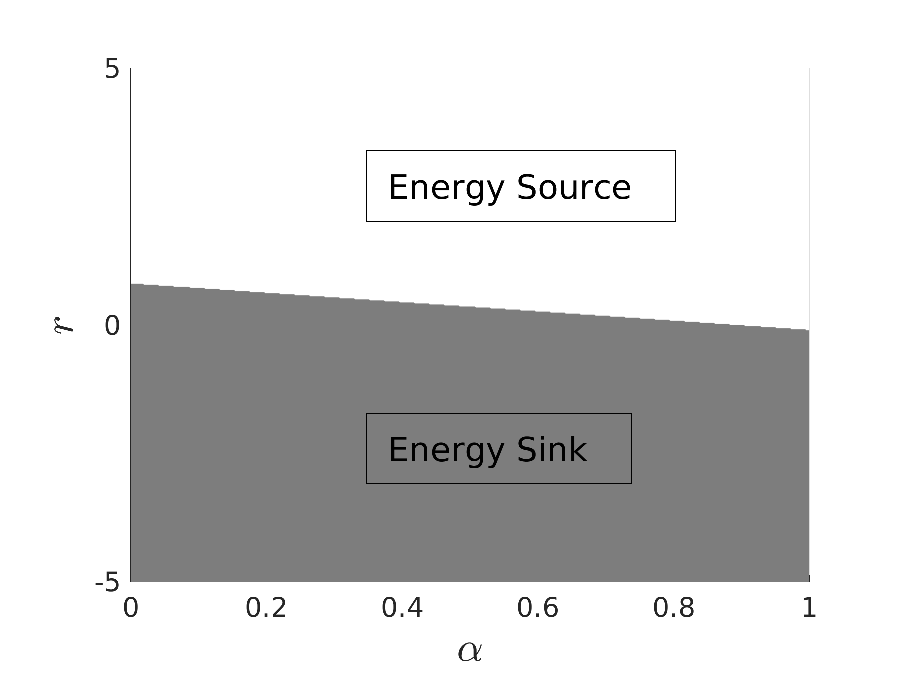
\includegraphics[width=3in]{filter_delta_energy}}
\caption{\small{Dissipative character of filtering for polynomial order $N=10$. Grey regions indicate the filter is dissipative while the white region indicates energy is being introduced into the flow by the filter.}}
\label{fig:filter_dissipation}
\end{figure}

The other aspect of the filtering operation which has been overlooked in the previous studies is its effect on the divergence-free condition. In order to asses the effects on divergence we revisit the double shear layer case studied in \cite{fischer01} and \cite{malm13}.

The flow case is setup in a two-dimensional domain $\Omega=[0,1]^{2}$ with doubly-periodic boundary conditions. The initial conditions are introduced as:
\begin{align}
 u_{0} &= 
 \begin{cases}
    	\tanh(\rho(y-0.25)),		& y \leq 0.5 \\
    	\tanh(\rho(0.75-y)),  	& y > 0.5
 \end{cases} \\
 v_{0} &= 0.05\sin(2\pi x),	\hspace{22pt}\forall\ x,y \nonumber
\end{align}
The domain is discretized with $16\times16$ spectral-element grid and each element uses $N=16$ Legendre polynomial modes, corresponding to $256$ points per element. The non-linear term is calculated using over-integration so as to preserve skew-symmetry of the advection term. The filtering stabilization procedure is also used to asses the effect of filtering on the divergence. $1\%$ of the last mode is filtered out at the end of each time-step. The tolerance of the solver for the divergence free condition is set to $10^{-10}$. Figure~\ref{fig:doubleshear_t0} shows the initial condition at time $t=0$ and Figure~\ref{fig:doubleshear_t2} shows the flow state at time $t=2$.

\begin{figure}[h]
	\centering
	\begin{subfigure}[b]{0.45\textwidth}
		\centering
		\includegraphics[width=1.1\columnwidth]{doubleshear_n16_t0}
		\caption{Initial vorticity at $t=0$}
		\label{fig:doubleshear_t0}
	\end{subfigure}
	\begin{subfigure}[b]{0.45\textwidth}
		\centering
		\includegraphics[width=1.1\columnwidth]{doubleshear_n16_t2}
		\caption{Vorticity at $t=2.0$}
		\label{fig:doubleshear_t2}
	\end{subfigure}
	\caption{Vorticity evolution for the double shear layer test case. }
	\label{fig:doubleshear_soln}
\end{figure}

Figure~\ref{fig:filter_divergence} shows the divergence of the flow field calculated before and after the application of the filter. The red line shows the divergence of the flow-filed after the pressure-correction step and the blue line indicates the divergence after the application of the filter. At the start of the simulation, when negligible energy is present in the last mode, the filter has very little impact on the divergence of the flow-field. However as the flow evolves and the energy in the smaller scales increase, violation of the divergence-free condition due to the action of the filter increases. This violation is substantial once the flow is fully developed, with the flow dropping nearly $6$ orders of magnitude in accuracy between the pressure-correction and the filtering step. This impact is surprisingly large. The case may be considered to be a stringent test with thin shear layers, which demand high resolution and thus even the small scales may contain dynamically significant energy. The situation however is representative of marginally resolved simulations where the smallest scales may still contain dynamically relevant energy, and thus filtering may have an unexpectedly large impact on the divergence-free condition of the flow-field.
\begin{figure}[h]
	\centerline{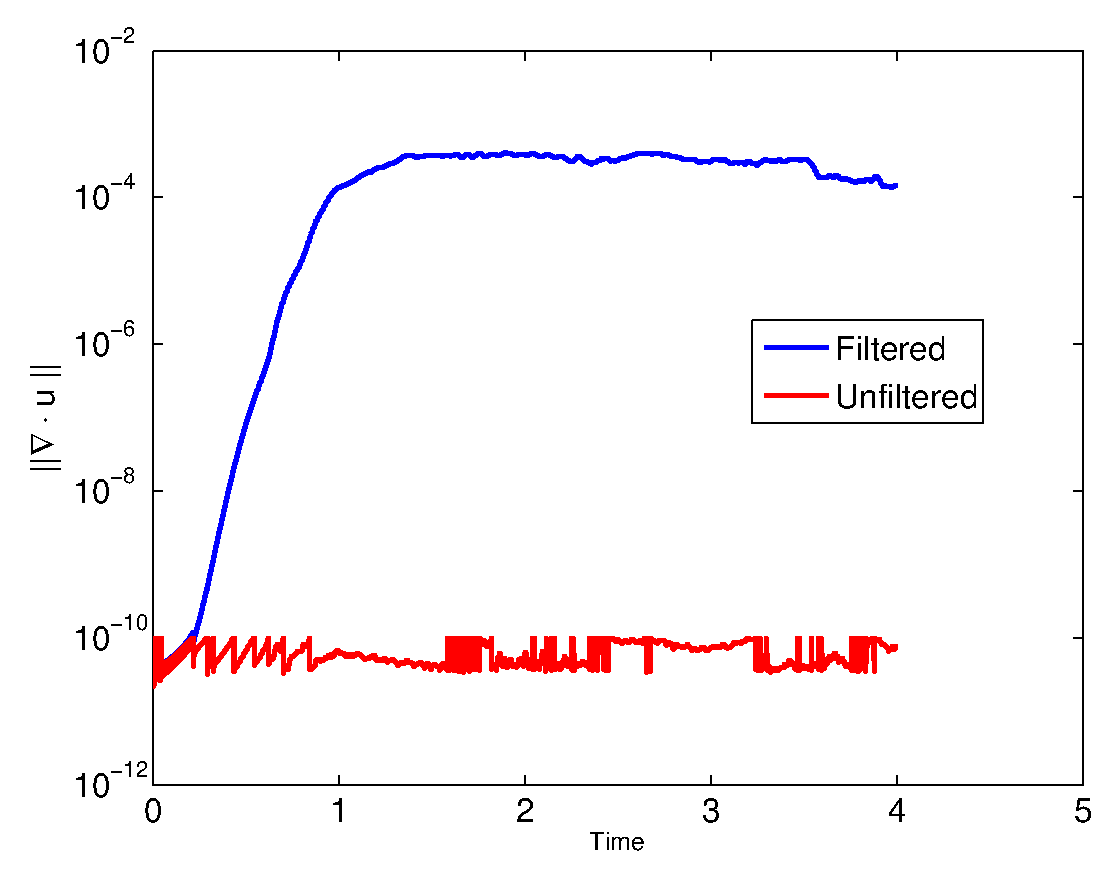
\includegraphics[width=3in]{divergence_filtered}}
	\caption{\small{The norm of the divergence after pressure correction and after filter application.}}
	\label{fig:filter_divergence}
\end{figure}

A puzzling aspect of the test as reported in the results of \cite{fischer01} and \cite{malm13} is that the case always needed some filter based stabilization. \cite{malm13} study the case with and without the use of over-integration for the non-linear term. They report that an order of magnitude lower filtering strength was needed when over-integration was used. However only over-integration did not ensure complete stabilization and the simulation experienced numerical instability at $T\sim6.7$ without filtering. \cite{malm13} attribute the destabilization to the finite accuracy of the divergence-free constraint, stating that even small errors would lead to numerical instability in the absence of dissipative terms (viscous or numerical) or stabilizing procedures (filtering). Although the authors do not report the tolerance to which the divergence free condition was satisfied. To check this again we run our test case with over-integration and without any filtering for a long duration. However contrary to the results obtained in \cite{malm13}, the simulation was stable (at least up to $T=20$). An explanation might be found when looking at the original test case reported in \cite{fischer01}. The authors there report using time steps such that the CFL number is between $1$ and $5$. The standard BDF3-K3 time-stepper would be unstable for these CFL numbers. This suggests that a characteristic time-stepping scheme may have been employed. We test the case by employing a the characteristic time-stepping scheme with over-integration but no filtering and indeed the simulation experienced numerical instabilities. This would implicate the characteristics time-stepper as the source of numerical instability. 

In retrospect, the results are to be expected. The use of consistent spaces for velocity and pressure avoids the spurious pressure oscillations. The absence of boundary conditions due to a doubly-periodic domain negates errors due to boundary terms, the use of over-integration dismisses aliasing errors as the source of instabilities and the spectral-element grid is perfectly Cartesian. Then as per the conclusion derived in \cite{malm13}, small divergence errors remain the obvious (known) source of numerical instability. However, these errors should be of the order of the specified solver tolerance for divergence. The (instantaneous) advection operator being real and skew-symmetric is a normal matrix (if evaluated completely using over-integration). Any violation of divergence-free condition of $O(\epsilon)$ can be regarded as a small perturbation to a normal matrix and one would expect a change in the eigenvalues to be of the same order $\epsilon$. Since in the ideal case the eigenvalues must lie on the imaginary axis with exactly zero real part, any perturbation due to numerical errors of order $O(\epsilon)$ would introduce new eigenvalues with a real part of $O(\epsilon)$. Thus a practical value for the solver tolerance of $10^{-8}$ would result in a advection matrix which would have eigenvalues with real parts of the order $10^{-8}$. Such a scenario creates an ever present numerical instability. However it should be an extremely weak instability, at least in such idealized test cases where other sources of instabilities are absent.

One can easily check the change of eigenvalues with varying degree of error in the advecting field. To do so we created a simple advection operator in Matlab following the spectral-element framework. A square domain with $\Omega=[0,1]^{2}$ is built and discretized using $3\times3$ spectral-elements which are further discretized using $10^{th}$ order Legendre polynomials. The advection operator is built on an over-integration grid with $19\times19$ grid points. The grid point spacing and weights for numerical integration correspond to the Gauss-Lobatto-Legendre points (GLL) for a polynomial of order $N_{d}=18$ resulting in the desired $18$ grid points for a complete integration of the convection term. Individual matrices are built independently for each spectral element and then a larger matrix for the whole system is built using direct stiffness summation. A simple sinusoidal divergence-free field can be used for building the $C\cdot\nabla$ matrix:
\begin{align}
\label{eqn:convection_op}
C_{x} &= 1.0 + 0.1\sin(2\pi x + 2\pi y) &+\epsilon\sin(2\pi x)\sin(2\pi y) \\
C_{y} &= 1.0 - 0.1\sin(2\pi x + 2\pi y) &+\epsilon\sin(2\pi x)\sin(2\pi y) \nonumber
\end{align}
When $\epsilon=0$ the field is analytically divergence free. Within the current numerical approximation the normalized divergence field defined as $||\nabla\cdot C|| = (\nabla\cdot C,\nabla\cdot C)/Volume$ is of the order $10^{-10}$. The parameter $\epsilon$ can thus be used to add a controlled perturbation to the advecting field and study the resulting change in eigenvalues. Figure~\ref{fig:spectra_eps0} and \ref{fig:spectra_eps-4} show the spectra of advection operator using $\epsilon=0$ and $\epsilon=10^{-4}$, resulting in divergence norms of the order $O(10^{-11})$ and $O(10^{-4})$ respectively. Tracking $\lambda_{max}$, defined as the eigenvalue with the largest real part, one can obtain how the instability of the advection operator changes with the variation of the divergence field. Figure~\ref{fig:lambda_dnorm} shows the change in $\lambda_{max}$ with $||\nabla\cdot C||$. As expected the trend is linear in a log-log scale with a slope of 1 across a variation of 8 orders of magnitude for $||\nabla\cdot C||$. This would suggest that relatively large divergence errors would be required for numerical instabilities to be caused by the advection term, as long as the term is evaluated completely. Of course as shown by \cite{malm13} and by \cite{kirby03}, the evaluation of this term without over-integration leads to instabilities in the absence of stabilization. These instabilities are much stronger than just divergence errors. Figure~\ref{fig:spectra_nodealias} shows the eigenvalue spectra for the advection operator (with $\epsilon=0$) evaluated on $11\times11$ GLL points in each element. The largest unstable eigenvalue is of the order $10^{-1}$, making the instability due to aliasing much stronger than the instabilities arising from the violation of the divergence-free condition.
\begin{figure}[h]
	\centering
	\begin{subfigure}[b]{0.45\textwidth}
		\centering
		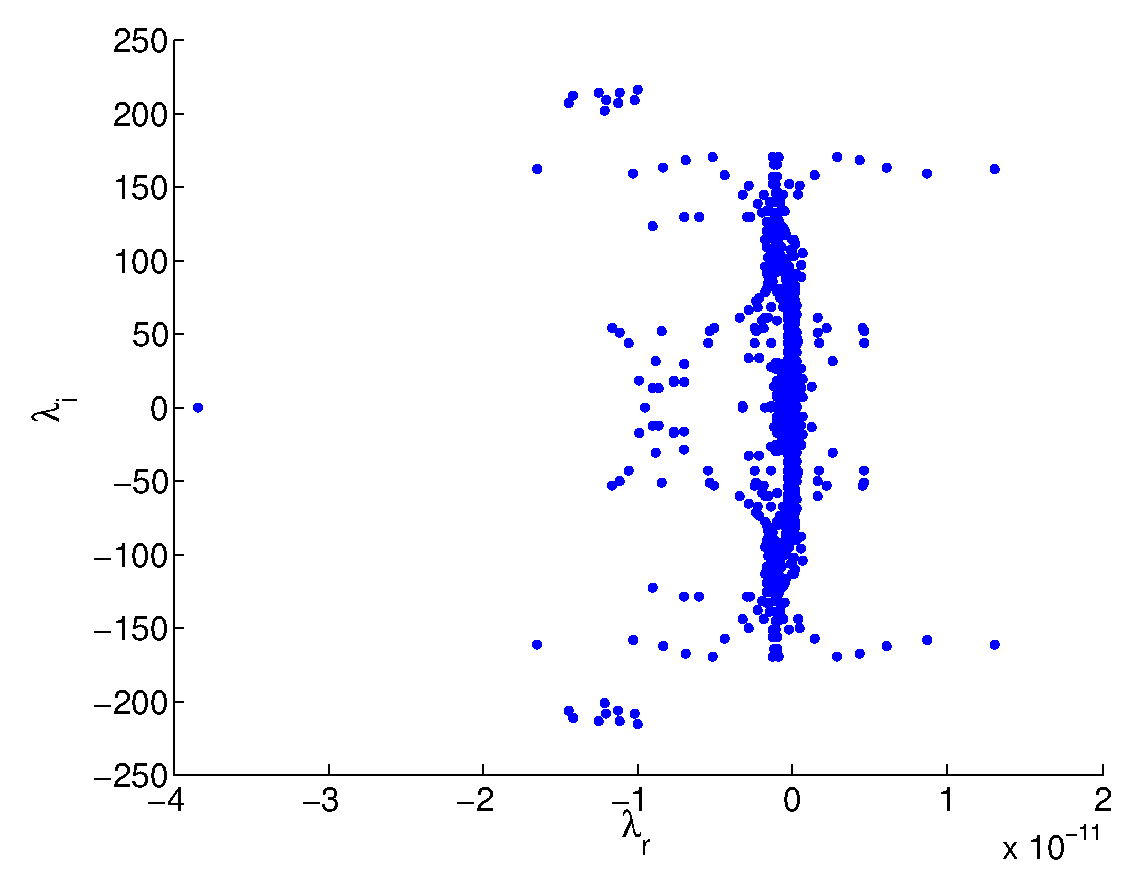
\includegraphics[width=1\columnwidth]{spectra_N10_Nxd18_nelv9_eps0}
		\caption{$||\nabla\cdot C|| \sim O(10^{-10})$}
		\label{fig:spectra_eps0}
	\end{subfigure}
	\begin{subfigure}[b]{0.45\textwidth}
		\centering
		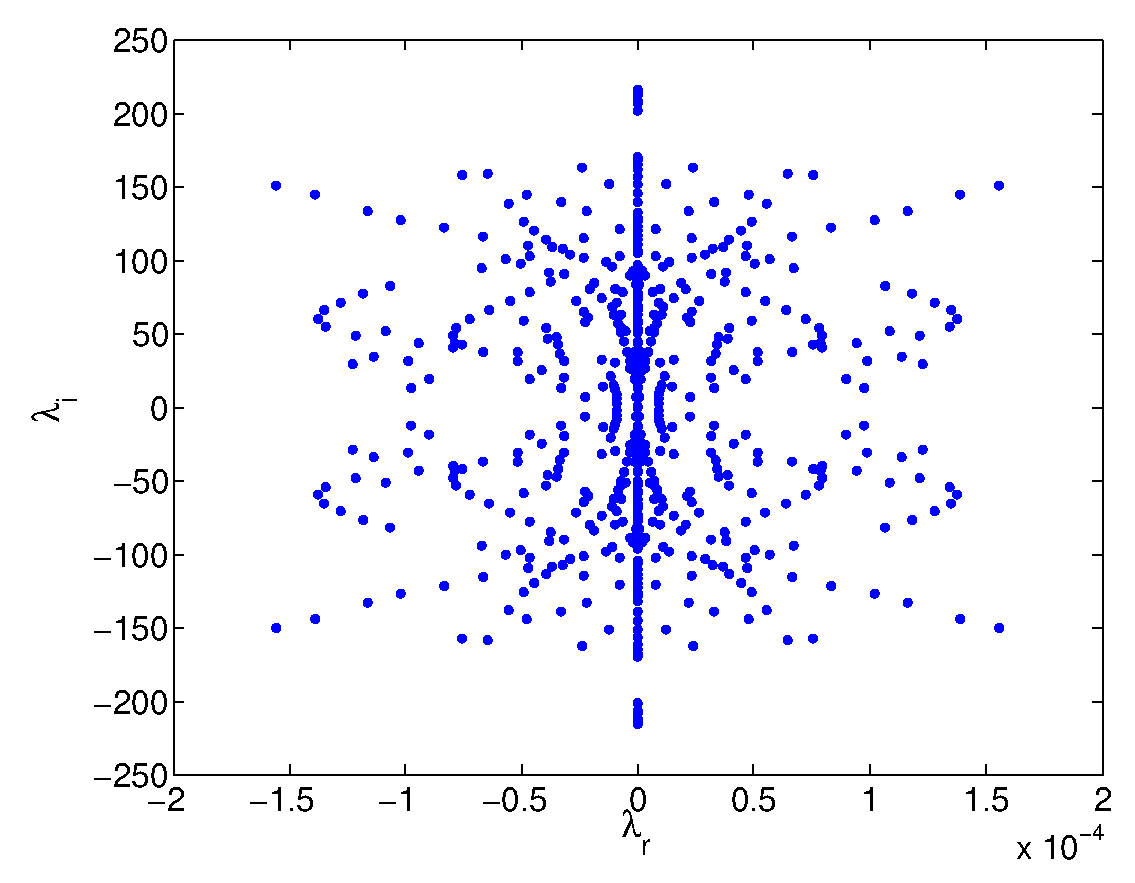
\includegraphics[width=1\columnwidth]{spectra_N10_Nxd18_nelv9_eps4}
		\caption{$||\nabla\cdot C|| \sim O(10^{-4})$}
		\label{fig:spectra_eps-4}
	\end{subfigure}
	\caption{Eigenvalue spectra for the advection operator with different divergence norms for a perturbed advecting field.}
	\label{fig:convection_spectra}
\end{figure}
\begin{figure}[h]
	\centerline{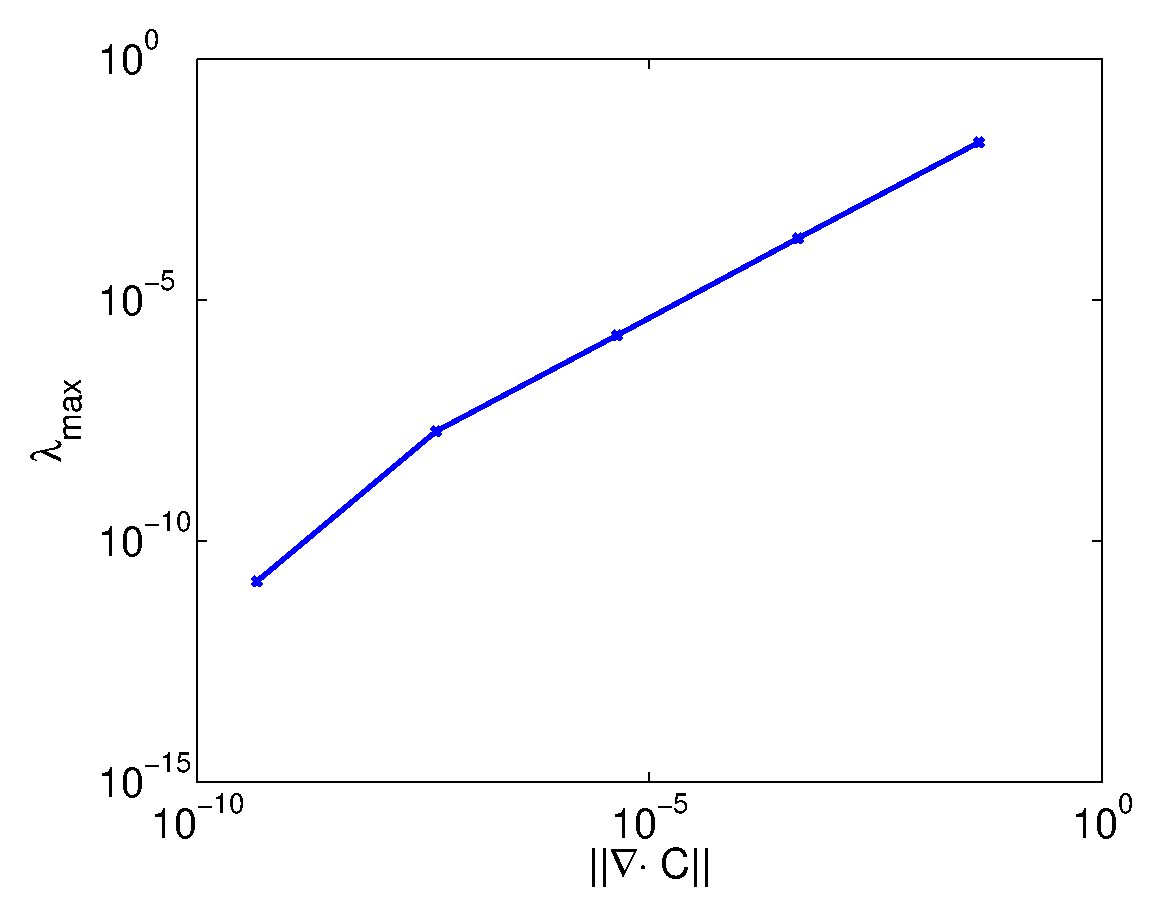
\includegraphics[width=2.5in]{N10_eig_dnorm}}
	\caption{\small{Variation of maximum real part of the eigenvalue spectrum with the norm of the divergence of the advection operator}}
	\label{fig:lambda_dnorm}
\end{figure}
\begin{figure}[h]
	\centerline{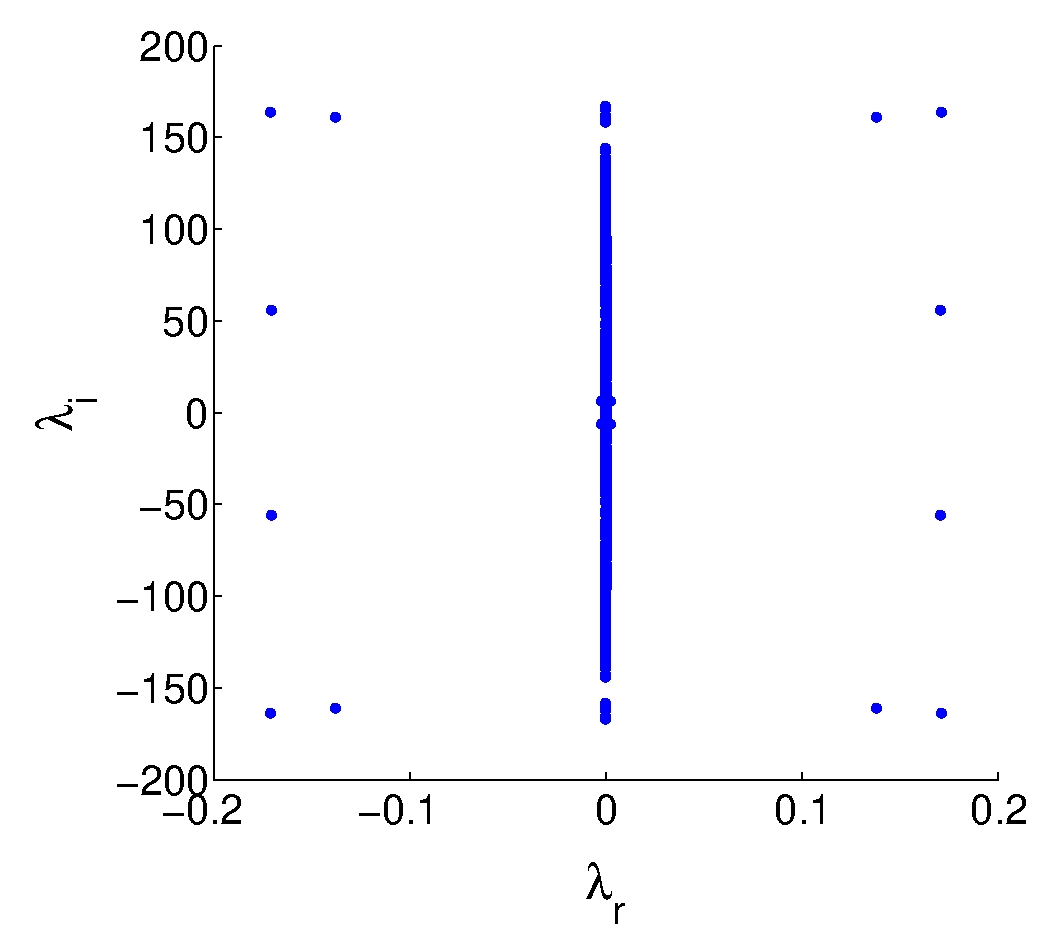
\includegraphics[width=2.5in]{spectra_nodealias_N10_Nd10}}
	\caption{\small{Eigenvalues for the advection term evaluated without over-integration}}
	\label{fig:spectra_nodealias}
\end{figure}
\cite{malm13} found that for the double shear layer case, the numerical instabilities first manifested in the thinnest part of the shear layers, thus concluding high shear regions necessarily need numerical stabilization. Since we do not experience any numerical instabilities using the BDF-EXT-k time stepping scheme, we further test this conclusion by reducing the resolution for the test case. We run the simulation with the same $16\times16$ spectral-elements but with polynomial orders of $N=11,7$ and $5$. These would lead to under-resolved shear layers. The under-resolution is strongly visible in the flow-field for the lowest polynomial order case of $N=5$. Figure~\ref{fig:vorticity_n6_t1} shows the vorticity in the flow field at time $t=1.0$ for $N=5$. However in all cases we find that the simulation does not experience any numerical instabilities (at least up till $t=20$) and additional stabilization was not required. The results indicate that in the absence of boundary terms and other sources of errors, under-resolution alone may not lead to numerical instabilities as long as the flow-field divergence remains small and the non-linear term is evaluated using complete over-integration. These results are consistent with those presented by \cite{kirby03} who found that they were able to simulate transition and turbulence in triangular ducts as well as turbulent channel flow simulations after employing over-integration but without additional flow stabilization.
\begin{figure}[h]
	\centering
	\includegraphics[width=3.5in]{doubleshear_n6_t1}
	\caption{\small{Vorticity at $t=1.0$ for the double shear layer case using polynomial order $N=5$}}
	\label{fig:vorticity_n6_t1}
\end{figure}


\section{Relaxation-term based stabilization}

In practical simulations over-integration errors may not be the only source of numerical instability and often it is found that simulations, especially those involving complex geometries or truncated domains require some amount to stabilization despite the use of over-integration. Filter-based stabilization has been an effective and efficient method to suppress such numerical instabilities. However the results of the previous section highlight some of the drawbacks of such a procedure. The loss of divergence free condition may be particularly severe for marginally resolved cases. In such a scenario, one may wish to look for an alternative method which preserves the advantages of explicit filtering, namely, efficiency and simplicity, while doing away with the potential drawbacks. One possible alternative in the context of the pressure-correction method is to perform the filtering procedure before the pressure-correction step. In the standard algorithm, the pressure-correction would follow a three-step procedure as follows: 
\begin{itemize}
	\item Velocity prediction $\rightarrow$ Pressure correction $\rightarrow$ Filtering.
\end{itemize}
A modified procedure would then follow:
\begin{itemize}
	\item Velocity prediction $\rightarrow$ Filtering $\rightarrow$ Pressure Correction.
\end{itemize}
This allows the filtering of the highest scales but leaves the solution unchanged after the divergence-free condition has been enforced. Such a procedure would remedy perhaps the most striking drawback of explicit filtering, which is the loss of divergence, while still retaining the simplicity and efficiency of explicit filtering operation. However the other drawbacks mentioned earlier, \textit{i.e} time-step dependence of filtered energy and the statistical nature of filter dissipation, still remain.

As it would turn out, there is an equally simple method that can resolve all the above mentioned deficiencies and is analogous to performing an explicit filtering procedure. As has been pointed out in \cite{stolz01} and \cite{schlatter04}, doing an explicit filtering operation is equivalent to doing an implicit time-relaxation. Formally, the two may be shown to be equivalent using a simple evolution equation \ref{eqn:NL_evolution}.
\begin{align}
\frac{\partial u}{\partial t} + \mathcal{F}(u) = 0
\label{eqn:NL_evolution}
\end{align}
Where $\mathcal{F}(u)$ is a (possibly non-linear) evolution operator.
The explicit filtering procedure may then be shown using a simple semi-discretized form of the evolution equation:
\begin{align}
u^{*} = u^{n} - \mathcal{F}(u^{n})\Delta t + O(\Delta t^{2})\nonumber \\
u^{n+1} =  \mathcal{G}(u^{*}) %& (\mathcal{G} - \text{Low pass filter.})
\label{eqn:NL_evolution_filtered}
\end{align}
Where $\mathcal{G}$ is a defined low-pass filter. As an alternate method, one may consider the same evolution equation supplemented by a relaxation-term as in equation~\ref{eqn:NL_evolution_rt}:
\begin{align}
\frac{\partial u}{\partial t} + \mathcal{F}(u) = \boldsymbol{-\chi \mathcal{H}(u)}
\label{eqn:NL_evolution_rt}
\end{align}
Which may be evolved using a time-splitting scheme:
\begin{align}
u^{*} = u^{n} -\mathcal{F}(u)\Delta t + O(\Delta t^{2})	\nonumber \\
u^{n+1} = u^{*} -\chi \mathcal{H}(u^{*})\Delta t + O(\Delta t^{2})
\label{eqn:NL_evolution_rt_1}
\end{align}
Taking the the parameter $\chi=1/\Delta t$ and $\mathcal{H}=\mathcal{(I-G)}$ to be the corresponding high-pass filter of $\mathcal{G}$, and substituting in equation \ref{eqn:NL_evolution_rt_1} one obtains:
\begin{align}
u^{n+1} = \mathcal{G}(u^{*}) + O(\Delta t^{2})
\label{eqn:NL_evolution_rt_2}
\end{align}
which is equivalent to the expression obtained in equation \ref{eqn:NL_evolution_filtered} to leading order of time discretization. \cite{stolz01} and \cite{schlatter04} interpret the relaxation-term as performing an equivalent low-pass filtering operation $\mathcal{G}$ every $1/(\chi\Delta t)$ time-steps. Alternately one may interpret this to mean that the relaxation-term procedure is equivalent to performing an explicit filtering operation with a filter strength of $(\chi\Delta t)$. 

Thus the ``filter-based stabilization'' operation proposed by \cite{fischer01} may be reformulated as an equivalent ``relaxation-term-based stabilization'', which we refer to as ``RT stabilization''. It can be easily incorporated into the Navier-Stokes by a simple addition of a relaxation-term on the right hand side. Thus the equivalent RT stabilized equation may be written as:
\begin{align}
\frac{\partial u}{\partial t} + u\cdot\nabla u = -\frac{\nabla p}{\rho} + \nu\nabla^{2}u -\chi\mathcal{H}(u) \\
\nabla\cdot u = 0
\label{eqn:rt_NS}
\end{align}
Where $\mathcal{H}(u)$ is a high-pass-filtered velocity field. The parameter $\chi$ may be used as a weighting parameter similar to the filter weight `$\alpha$' used in \cite{fischer01} and \cite{malm13}. Such a formulation immediately provides us with two advantages over the explicit filtering operation. Firstly, since there are no more explicit filtering operations after the pressure-correction step, the velocity field remains divergence free. Secondly, with the RT now part of the evolution equations, for a fixed $\chi$ and $\mathcal{H}$ the physical energy drain provided by the RT should be independent of the chosen time-step (as long as numerical stability is ensured). The final aspect of the stabilization concerning the dissipative character of the RT requires more constraints. When $\mathcal{H}$ is chosen to be positive semi-definite, and $\chi$ is a positive constant, the relaxation-term is purely dissipative. However with spatially varying $\chi$ and $\mathcal{H}$ the relaxation-term may be non-dissipative \citep{stolz03}.
\subsection{RT parameters}
\cite{malm13}, in the context of spectral-elements, describe a simple transfer function $\mathcal{G}$ defined for a variable in a one-dimensional domain $\Omega=[-1, 1]$ such that the filtering operation takes the simple form: 
\begin{align}
\bar{u}_{N}(x) = \mathcal{G}(u_{N}(x)) = \sum_{k=0}^{N}\sigma_{k}a_{k}\phi_{k}(x)
\end{align}
Where $\phi_{k}$ is the basis function and the definition of $\sigma_{k}$ describes the low-pass filter function $\mathcal{G}$ which takes the form:
\begin{align}
\sigma_{k} &=
	\begin{cases}
	1 - \alpha\left(\frac{k-k_{c}}{N-k_{c}}  \right)^{2}, & k>k_{c} \\
	1, & k\le k_{c}
	\end{cases}
\end{align}
Where $N$ is the number of modes in the spectral-element discretization and $k_{c}$ is the cut-off mode in spectral space used for building the filter. Amplitudes for modes $k\le k_{c}$ are unaffected by the filter operation. $\alpha$ is the filter weight such that $0\le\alpha\le1$. In keeping with our analysis earlier, we may define the corresponding high-pass filter $\mathcal{H}$ for the RT as:
\begin{align}
\mathcal{H}(u_{N}(x)) &= \sum_{k=0}^{N}\gamma_{k}a_{k}\phi_{k}(x) \\
\gamma_{k} &=
\begin{cases}
	\left(\frac{k-k_{c}}{N-k_{c}}  \right)^{2}, & k>k_{c} \\
	0, & k\le k_{c}
\end{cases}
\end{align}
Where the parameter $\alpha$ is absorbed into $\chi$ which acts as an RT strength term. To formally have the same operation as the explicit filter, the value of $\chi$ can be set to $\chi=(\alpha/\Delta t)$. This is in agreement with our earlier interpretation that the RT procedure is equivalent to performing a low-pass filter operation every time-step with a strength of $(\chi\Delta t)$. Using this value we get $\chi\Delta t = \alpha$ and thus we recover the correct weighting for the equivalent explicit filter operation. 

The basis functions $\phi$ used for the definition of $\mathcal{H}$ however is different from the one used by \cite{malm13} who use the transformed basis functions described by \cite{boyd98} which are described in equation~\ref{eqn:boyd}. Using this basis function however, the form of $\mathcal{H}$ is not semi-positive definite and thus the relaxation term is not purely dissipative. This is rather expected from our earlier results which show that the explicit filter operation using such a transformed basis has a substantial parameter range where it acts as an energy source. The equivalent RT formulation then can not be purely dissipative. We use the Legendre polynomials as the basis functions (for a Legendre-spectral-element method) for building the RT which makes $\mathcal{H}$ semi-positive definite. Thus for $\chi>0$ the relaxation term $-\chi\mathcal{H}(u)$ is always purely dissipative.

\subsection{Stability and parameter range}
The action of the RT can be inferred from the change in eigenvalues of the system due to the added stabilization. As an illustration we build the system matrices using the simple $3\times3$ spectral-element grid in Matlab for a linear advection operator stabilized by a relaxation-term. The advection operator is built using the parameters in equation~\ref{eqn:convection_op}. We set $\epsilon=10^{-2}$ so that the operator now models a numerically unstable system with positive eigenvalues. The eigenvalues of the unstable system without the addition of a relaxation term are shown in figure~\ref{fig:spectra_conv_eps2}. As expected, there are unstable eigenvalues with positive real part of order $O(10^{-2})$. With the addition of an RT as defined earlier, with $k_{c}=10$ and $\chi=0.4$ causes the eigenvalues to shift towards the negative real plane (figure~\ref{fig:spectra_rhs_eps2}). In the example shown here, the instability appears to be completely suppressed and the largest real part of the eigenvalues of the resulting system is zero. The overall system is more dissipative as evidenced by the general negative shift of the real part of the eigenvalues.
\begin{figure}[h]
	\centering
	\begin{subfigure}[b]{0.45\textwidth}
		\centering
		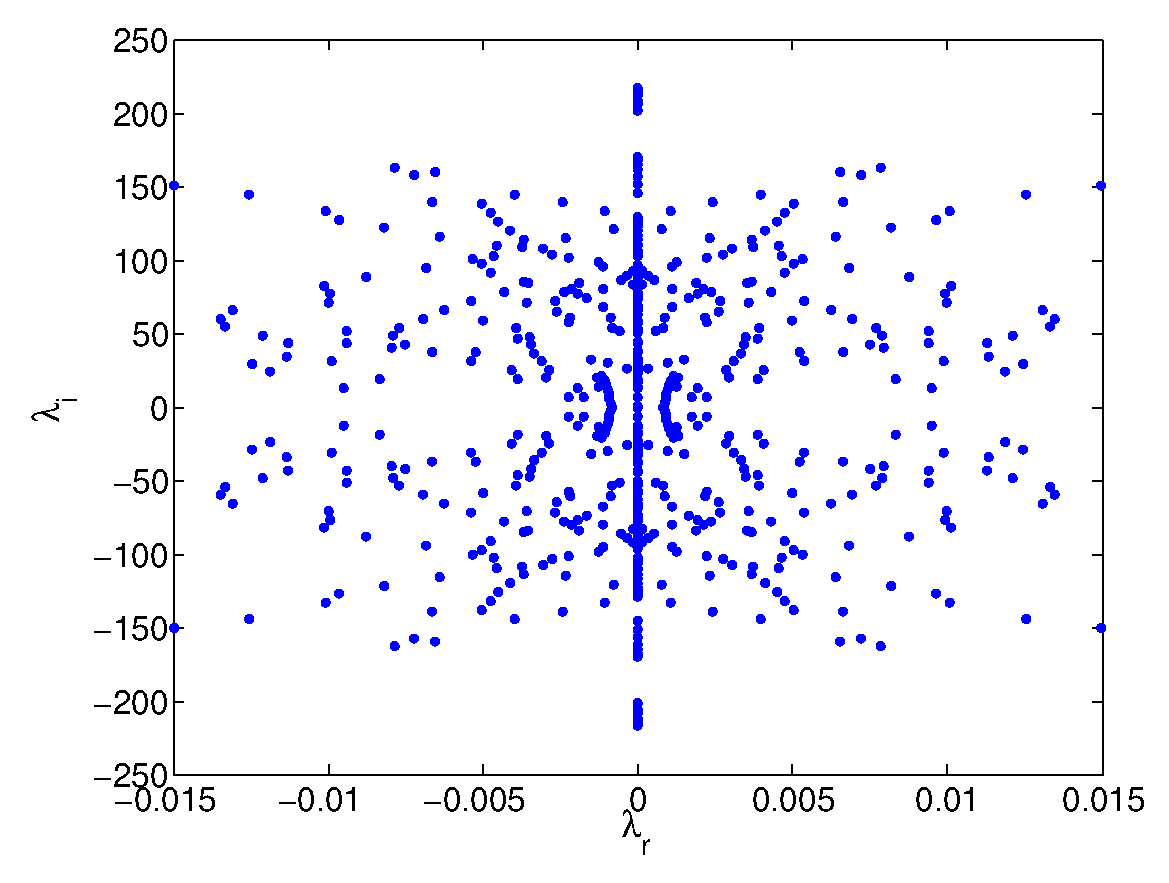
\includegraphics[width=1\columnwidth]{spectra_conv_N10_Nxd18_nelv9_eps2}
		\caption{$||\nabla\cdot C|| \sim O(10^{-2})$}
		\label{fig:spectra_conv_eps2}
	\end{subfigure}
	\begin{subfigure}[b]{0.45\textwidth}
		\centering
		\includegraphics[width=1\columnwidth]{spectra_rhs_N10_Nxd18_nelv9_eps2}
		\caption{Stabilized Eigenvalues.}
		\label{fig:spectra_rhs_eps2}
	\end{subfigure}
	\caption{Comparison of eigenvalues for an unstable system (a) with $||\nabla\cdot C|| \sim O(10^{-2})$ and a system stabilized using a relaxation-term (b)}
	\label{fig:rt_spectra}
\end{figure}

While the RT clearly has a stabilizing effect on the system, it can also be destabilizing for a certain range of parameters. From figure~\ref{fig:spectra_rhs_eps2} one can notice some eigenvalues of the stabilized system have a large negative shift with the smallest real part being $\lambda_{r}^{min}=-0.4$. As it turns out this particular eigenvalue sets the stability limits of the RT stabilization approach. For a particular temporal discretization such as the BDF-EXT-3, the region of stability may cover a finite region of the negative plane. For a system with eigenvalues such that $\lambda\Delta t$ falls outside the stability region of the time-stepping scheme, the system becomes numerically unstable. The scaled eigenvalues with varying values of the parameter $\chi\Delta t$ (and $k_{c}=1$) are shown in figure~\ref{fig:rt_stability} with a black line enveloping the region of stability for a BDF-EXT-3 temporal discretization scheme. As the strength of the RT stabilization is increased by varying $\chi$, the eigenvalues become more negative and the dissipative character of the stabilization procedure becomes stronger. Eventually as $\chi\Delta \approx 1$ the stabilization procedure itself becomes numerically unstable and the time-step needs to be reduced in order to render the simulation numerically stable again. The analysis is exemplified using the BDF-EXT-3 scheme but the concept generalizes to other schemes and the limit of stability will be governed by the stability region of the respective schemes.
\begin{figure}[h]
	\centering
	\begin{subfigure}[b]{0.45\textwidth}
		\centering
		\includegraphics[width=1\columnwidth]{spectra_chidt_001}
		\caption{$\chi\Delta t=0.01$}
		\label{fig:spectra_chidt001}
	\end{subfigure}
	\begin{subfigure}[b]{0.45\textwidth}
		\centering
		\includegraphics[width=1\columnwidth]{spectra_chidt_010}
		\caption{$\chi\Delta t=0.10$}
		\label{fig:spectra_chidt01}
	\end{subfigure}
	\begin{subfigure}[b]{0.45\textwidth}
		\centering
		\includegraphics[width=1\columnwidth]{spectra_chidt_050}
		\caption{$\chi\Delta t=0.50$}
		\label{fig:spectra_chidt050}
	\end{subfigure}
	\begin{subfigure}[b]{0.45\textwidth}
		\centering
		\includegraphics[width=1\columnwidth]{spectra_chidt_100}
		\caption{$\chi\Delta t=1.00$}
		\label{fig:spectra_chidt100}
	\end{subfigure}	
	\caption{Changes in eigenvalues with varying filter strength $\chi\Delta t$ with $k_{c}=10$.}
	\label{fig:rt_stability}
\end{figure}
This condition limits the parameter range for which a relaxation-term type stabilization can be used. Practical values of the $\chi$ parameter should not reach such a limit. To compare with an explicit filtering case, practical values of the filter strength vary between $0\le\alpha\le0.3$ which correspond to $0\le\chi\Delta t\le0.3$. \cite{fischer01} apply the filtering procedure with $\alpha=1.0$ and note that lower values of $\alpha$ are preferable. Should one find that the dissipation provided at low values of $\chi$ is not enough, the alternative would be to change the cut-off wavenumber $k_{c}$. This increases the added dissipation by the relaxation-term but does not substantially change the stability limits. Figure~\ref{fig:rt_stability_k8} shows the change in eigenvalues with different $\chi\Delta t$ using the cut-off mode number as $k_{c}=8$. The system is clearly more dissipative with many more eigenvalues with large negative real parts. However the approach to numerical instability remains approximately the same at $\chi\Delta t\approx 1.0$.
\begin{figure}[h]
	\centering
	\begin{subfigure}[b]{0.45\textwidth}
		\centering
		\includegraphics[width=1\columnwidth]{spectra_chidt_001_k8}
		\caption{$\chi\Delta t=0.01$}
		\label{fig:spectra_chidt001_k8}
	\end{subfigure}
	\begin{subfigure}[b]{0.45\textwidth}
		\centering
		\includegraphics[width=1\columnwidth]{spectra_chidt_010_k8}
		\caption{$\chi\Delta t=0.10$}
		\label{fig:spectra_chidt01_k8}
	\end{subfigure}
	\begin{subfigure}[b]{0.45\textwidth}
		\centering
		\includegraphics[width=1\columnwidth]{spectra_chidt_050_k8}
		\caption{$\chi\Delta t=0.50$}
		\label{fig:spectra_chidt050_k8}
	\end{subfigure}
	\begin{subfigure}[b]{0.45\textwidth}
		\centering
		\includegraphics[width=1\columnwidth]{spectra_chidt_100_k8}
		\caption{$\chi\Delta t=1.00$}
		\label{fig:spectra_chidt100_k8}
	\end{subfigure}	
	\caption{Changes in eigenvalues with varying filter strength $\chi\Delta t$ with $k_{c}=8$.}
	\label{fig:rt_stability_k8}
\end{figure}

It is important to note that such a formulation is very similar to the RT-3D approach used by \cite{schlatter04} in the context of large-eddy simulations of transitional flows. In the study the authors compare different variants of the ADM-RT (approximate deconvolution model with relaxation term) for transitional and turbulent regimes. In the RT-3D variant the non-linear terms are computed without the deconvolution procedure and hence only the relaxation-term is used for modeling the sub-grid stresses. In the current study we are only concerned with the relaxation-term procedure in the context of numerical stabilization. 

\subsection{Double shear layer}
We test the RT stabilization in the 2D model test case of double shear layer as done in by \cite{fischer01} and \cite{malm13} for a several different parameters. Quite expectedly the procedure successfully stabilizes the simulations. We show the results of only one test case when no over-integration is employed, which would be the most stringent test case for stabilization. We ran the test using a $16\times16$ spectral-element grid with $N=16$ Legendre modes in each spectral-element. The RT parameters of $\chi=1.5\times10^{-3}$ (corresponding to $\chi\Delta t=0.3$) and $k_{c}=15$ were used. Figure~\ref{fig:rt_n15_t2} shows the vorticity in the field at $t=2.0$ where the thin shear layers are clearly visible. The simulation ran without numerical instabilities up to $t=20$.
\begin{figure}[h]
	\centering
	\includegraphics[width=3.0in]{visit_rt_t2}
	\caption{\small{Vorticity at $t=2.0$ for the double shear layer case using polynomial order $N=16$ without over-integration and using a relaxation-term stabilization.}}
	\label{fig:rt_n15_t2}
\end{figure}


\section{Conclusion}
We reassess the filter-based stabilization proposed by \cite{fischer01} and find that despite its appealing simplicity and efficiency, it suffers from several drawbacks, the most striking of which is the loss of the divergence-free condition of the flow field. In marginally resolved simulations, this loss may be severe as in our model test case where 6 orders of accuracy was lost for the divergence-free condition. Two other drawbacks are the time-step dependence of the filtered energy and the statistical character of the filter dissipation. An alternate formulation for stabilization is proposed called the ``relaxation-term-based stabilization'' or RT stabilization, which is closely related to the explicit filtering operation. With appropriate parameters can be shown to be equivalent to an explicit filter operation to leading order of time discretization. The procedure stabilizes the numerical method without destroying the divergence-free condition and for an appropriately built high-pass filter $\mathcal{H}$ the term has the quality of being purely dissipative. Moreover, the stabilization is now part of the evolution equations, and thus the energy drain due to relaxation-term is independent of the chosen time-step. Limits of the stabilization are also shown and under certain parameters the stabilization itself becomes numerically unstable. However the procedure is stable under the standard parameter ranges which may be expected for numerical stabilization. Test cases with the double shear layer shows the relaxation-term is able to stabilize the numerical simulation even in the absence of over-integration, which corresponds to a fairly stringent case of numerical stability in the presence of negligible viscosity.




%\begin{footnotesize}
%\bibliography{licentiate}\bibliographystyle{jfm}
%\end{footnotesize}

%\end{document}



%------------------------------------------------------------------------------
% Bibliography
%------------------------------------------------------------------------------
%
%\clearpage
\bibliographystyle{jfm}
\bibliography{licentiate}
%
%\IfFileExists{stabilization/paper.bbl}{%------------------------------------------------------------------------------
% Define title, author(s), affiliation and publishing status
%
\papertitle[Rexalation-term stabilization] % Short title used in headlines (optional)
{%
  A re-examination of filter-based stabilization for spectral element methods% THE COMMENT SYMBOL AT THE END OF THIS LINE IS NEEDED
}%
%
\papertoctitle{Relaxation-term-based stabilization} % Title for toc
%
\paperauthor[Negi P. S.] % Short authors used in headlines and List Of Papers
{%
  P. S. Negi %$^{1,2}$, P. Schlatter$^{1,2}$, A. Hanifi$^{1}$ and D. S. Henningson$^{1,2}$%
}%
%
%\listpaperauthor{A. Skywalker \& D. Vader}% (optional) Short authors used in List Of Papers
%
\paperaffiliation
{%
%  $^1$ Linn\'e FLOW Centre, KTH Mechanics, S-100 44 Stockholm, Sweden\\
%  $^2$ Swedish e-Science Research Centre (SeRC), SE-100 44, Stockholm, Sweden%
  Linn\'e FLOW Centre, KTH Mechanics, S-100 44 Stockholm, Sweden\\
  Swedish e-Science Research Centre (SeRC), SE-100 44, Stockholm, Sweden%
}%
%
\paperjournal[Gal. Empire Publ.] % Short publish info used in List Of Papers
{%
	Galactic Empire Publications%
}%
%
\papervolume{42}%
%
\papernumber{2}%
%
\paperpages{1--10}%
%
\paperyear{3639}%
%
\papersummary%
{% Insert summary of the paper here (used in introduction) 
	The implications of concurrent archetypes have been far-reaching and
	pervasive. Given the current status of heterogeneous technology,
	cyberinformaticians daringly desire the key unification of the Turing
	machine and erasure coding. We explore new decentralized information,
	which we call Tuna.
}%
%
\graphicspath{{stabilization/imgs/}}%
%
%
%===============================================================================
%                            BEGIN PAPER
%===============================================================================
%
\begin{paper}

\makepapertitle

%------------------------------------------------------------------------------
% Abstract
%------------------------------------------------------------------------------
%
\begin{paperabstract}
	We revisit the ``filter-based stabilization'' approach proposed by \cite{fischer01} and find that it suffers from several drawbacks. In particular the ``evolve and filter'' approach causes a violation of the divergence-free condition which can be particularly severe in the cases of marginally resolved flows. Moreover the form of the filtering operation causes the filter to not be purely dissipative. Instead of a filter-based approach we propose to use a ``relaxation-term-based stabilization'' which we refer to as an RT stabilization, which is very closely related to the explicit filtering operation. The method retains the advantages of simplicity and efficiency of a filter based approach while also remedying the above mentioned drawbacks. Parameter limits of such a stabilization procedure are explored and the method is shown to be effective within the practical parameter ranges.
\end{paperabstract}


%------------------------------------------------------------------------------
% Article
%------------------------------------------------------------------------------
%
\input{stabilization/article.tex}


%------------------------------------------------------------------------------
% Bibliography
%------------------------------------------------------------------------------
%
%\clearpage
\bibliographystyle{jfm}
\bibliography{licentiate}
%
%\IfFileExists{stabilization/paper.bbl}{\input{stabilization/paper.bbl}}{}

%===============================================================================
%                            END PAPER
%===============================================================================
\end{paper}
}{}

%===============================================================================
%                            END PAPER
%===============================================================================
\end{paper}
}{}

%===============================================================================
%                            END PAPER
%===============================================================================
\end{paper}
}{}

%===============================================================================
%                            END PAPER
%===============================================================================
\end{paper}
